\documentclass[11pt]{article}
\usepackage{hyperref}
\usepackage{graphicx}
\usepackage{underscore}
\usepackage{xcolor}
\usepackage{color}
\usepackage{cancel}
\usepackage{ulem}
\usepackage{caption}
\usepackage{listings}
\usepackage{subcaption}
\usepackage{devanagari}

\setlength{\textwidth}{17.5cm}
\setlength{\textheight}{23.2cm}
\setlength{\hoffset}{-2.0cm}
\setlength{\voffset}{-2.5cm}

\newcommand{\rcancel}[1]{\renewcommand\CancelColor{\color{red}}\xcancel{#1}}
\newcommand{\webpage}{http://beta.sumeetsinha.in/gmESSI}
\definecolor{dkgreen}{rgb}{0,0.6,0}
\definecolor{gray}{rgb}{0.5,0.5,0.5}
\definecolor{mauve}{rgb}{0.58,0,0.82}
\definecolor{ltgray}{rgb}{0.98,0.98,0.98}
\definecolor{grayish}{rgb}{0.85, 0.85, 0.85}
\definecolor{darkpink}{rgb}{0.858, 0.188, 0.478}

% \input{essi_listings_options.tex}

\lstset{frame=single,
  backgroundcolor=\color{ltgray},
  aboveskip=3mm,
  belowskip=3mm,
  showstringspaces=false,   
  columns=flexible,
  basicstyle = \ttfamily,
  columns=fullflexible,
  numberstyle=\tiny\color{black},
  keywordstyle=\color{blue},
  commentstyle=\color{gray},
  stringstyle=\color{mauve},
  breaklines=true,
  numbers=left,
  breakatwhitespace=true,
  tabsize=3,
  %rulecolor=\color{mauve},
}

\lstset{escapeinside={<@}{@>}}

\title{gmESSI Manual}
% \author{Sumeet Kumar Sinha \\ {\dn \7{s}Emt \7{k}mAr Es\306whA }  }
\date{\today}

\begin{document}

\maketitle

\tableofcontents
\newpage



%%%%%%%%%%%%%%%%%%%%%%%%%%%%%%%%%%%%%%%%%%%%%%%%%%%%%%%%%%%%%%%%%%%%%%%%%%%%%%%
%%%%%%%%%%%%%%%%%%%%%%%%%%%%%%%%%%%%%%%%%%%%%%%%%%%%%%%%%%%%%%%%%%%%%%%%%%%%%%%
\section{Introduction} 


\textbf{gmESSI}  pronounced  as  \textit{[g-mESSI]}  is  an  acronym for gmsh (a
three-dimensional   finite   element  mesh  generator  with  built-in  pre-  and
post-procESSIng        facilities)        to        ESSI        (UC        Davis
Earthquake-Soil-Structure-Interaction   Simmulator)   Finite   Element   Program
Translator.  The  translator  has been developed in C++ language by Sumeet Kumar
Sinha,  a  PhD  student  under  Prof.  Boris Jeremic at University of California
Davis. The primary aim is to provide an easy, handy and powerfool pre-procESSIng
tool   to  develop  FEA  models  and  make  them  interface  with  various  ESSI
functionalities.    The    gmESSI    Translator    Package    consist   of   the
\textit{Translator,  Python  module, a Sublime plugin and its manual}. The whole
package  can be downloaded from \href{https://github.com/SumeetSinha/gmESSI}
{here}. The sublime plugin  \textit{\textbf{[gmESSI-gmsh Tools]}} can   be   
downloaded   from  Package  Control  or  from
\href{https://github.com/SumeetSinha/gmESSI-SublimePlugin}{GitHub}.\\ 

\textbf{Note:-  \textit{\underline{However  smart  a translator is, never fully
trust it!} Always  check  out the output files generated to see whether the
conversion made was correct or not.}}


%%%%%%%%%%%%%%%%%%%%%%%%%%%%%%%%%%%%%%%%%%%%%%%%%%%%%%%%%%%%%%%%%%%%%%%%%%%%%%%
%%%%%%%%%%%%%%%%%%%%%%%%%%%%%%%%%%%%%%%%%%%%%%%%%%%%%%%%%%%%%%%%%%%%%%%%%%%%%%%
%%%%%%%%%%%%%%%%%%%%%%%%%%%%%%%%%%%%%%%%%%%%%%%%%%%%%%%%%%%%%%%%%%%%%%%%%%%%%%%
\section{Getting Started} 

The  translator utilizes the \textbf{Physical and Entity group} concept of Gmsh,
which  gets  imprinted in the mesh \textbf{.msh} file and then manupulates these
groups  to convert the whole mesh to ESSI commands. Thus, making physical groups
is  the key to conversion for this Translator. The Translator basically provides
some  strict  syntax for naming these Physical Groups using \textbf{\textit{tags
and  gmESSI  commands}}  which provides it the information about how and what to
convert.  \textit{The  translator  is made so general that any other FEM program
can  use  it with little tweaks to have their own conversion tool}. A quick look
at some important features of the program are:


\begin{itemize}

  \item[$\bullet$]  It  has  a lot of  \textbf{predefined commands} which do the
  conversion  at  the  blink  of an eye. These commands make it easier to define
  elements, boundary conditions, contacts, fixities, loads ....
  
  \item[$\bullet$]  It  provides a python module \textbf{gmESSI} using which the
  user  can  program  and  make  their  own  conversions.  

  \item[$\bullet$] The \textbf{gmESSI sublime plugin} makes it easy by providing 
  syntax colouring and text-completion for gmsh as well as gmESSI commands. The 
  plugin can be installed by the name of \textbf{gmESSI-gmsh Tools} from sublime 
  package control. The repository for this plugin can be found at 
  \href{https://github.com/SumeetSinha/gmESSI-SublimePlugin}{GitHub}
  
  \item[$\bullet$]  The  translator uses a \textit{\textbf{ \href
  {https://github.com/SumeetSinha/gmESSI/blob/master/mapping.fei}
  {mapping.fei}}} file to
  check  for  its command syntax and conversion. A user can easily add a command
  in  \textbf{mapping.fei}  and  it  would  get  reflected  automatically in the
  translation.

\end {itemize}

%%%%%%%%%%%%%%%%%%%%%%%%%%%%%%%%%%%%%%%%%%%%%%%%%%%%%%%%%%%%%%%%%%%%%%%%%%%%%%%
%%%%%%%%%%%%%%%%%%%%%%%%%%%%%%%%%%%%%%%%%%%%%%%%%%%%%%%%%%%%%%%%%%%%%%%%%%%%%%%
\subsection{Installation Process}

The  Translator  have  its dependencies on Octave (3.2 or higher), Boost(1.58 or
higher),  (Python  2.7  or higher) and g++ (4.9 or higher) commpiler. One should
make  sure  to  have  them  before  compiling  it.  A  quick  reference to these
dependencies are

\begin{itemize}

  \item[$\bullet$] \textbf{Boost}:: It can be downloaded
  \\url{http://www.boost.org/users/download}. Just follow the installation
  steps as provided on the site.

  \item[$\bullet$] \textbf{Octave}:: The package is available at
  \url{http://packages.ubuntu.com/search?keywords=octave} for different
  ubuntu versions. Make sure to comment all the \textit{warnings} of file
  \textit{\textbf{ov-typeinfo.cc}} before compiling the package.
  \textbf{Alternatively}, one can try to install liboctave by running
  \textbf{sudo apt-get install liboctave-dev} but the user would get warnings
  from octave while running the program.

  \item[$\bullet$] \textbf{Python}:: The ubuntu users can install it using
  \textbf{sudo apt-get install python-dev}.

  \item[$\bullet$] \textbf{g++}:: the latest version of the gnu compiler can
  be installed on linux machine by running the following commands.

  \textbf{sudo apt-get install build-essential}\\   
  \textbf{sudo add-apt-repository ppa:ubuntu-toolchain-r/test} \\ 
  \textbf{sudo apt-get update}\\
  \textbf{sudo apt-get install gcc-4.9 g++-4.9 cpp-4.9 gfortran-4.9} 

\end{itemize}

Installation of the gmESSI translator is really easy. Just follow the steps as
shown below.\href{http://beta.sumeetsinha.in/gmESSI/Install.sh}{ Script}

\begin{lstlisting}[language=bash]
# go to the folder where you want to store the gmESSI software and run this script
#Download the latest version of the package from github
git clone https://github.com/SumeetSinha/gmESSI.git
cd ~/gmESSI

# install the package 
make
make install

\end{lstlisting}

%%%%%%%%%%%%%%%%%%%%%%%%%%%%%%%%%%%%%%%%%%%%%%%%%%%%%%%%%%%%%%%%%%%%%%%%%%%%%%%
\subsection {Running gmESSI}

gmESSI  can  be invoked from the bash terminal by typing \textbf{gmESSI}. It
can take  \textit{one or multiple} \textbf{XYZ.msh} files as an argument and
convert them to ESSI files in their respective folders names as
\textbf{XYZ\_ESSI\_Simulation} placed at the execution location.
\href{http://beta.sumeetsinha.in/gmESSI/Examples/Example1/Example1.geo}{
Example1.geo}
\href{http://beta.sumeetsinha.in/gmESSI/Examples/Example1/Example1.msh}{
Example1.msh }


%%%%%%%%%%%%%%%%%%%%%%%%%%%%%%%%%%%%%%%%%%%%%%%%%%%%%%%%%%%%%%%%%%%%%%%%%%%%%%%
%%%%%%%%%%%%%%%%%%%%%%%%%%%%%%%%%%%%%%%%%%%%%%%%%%%%%%%%%%%%%%%%%%%%%%%%%%%%%%%
\subsubsection{In Terminal}

\begin{lstlisting}[language=bash,backgroundcolor=\color{grayish}]
$ gmessi ./Example1.msh
<@\textcolor{blue}{Message::Files converted to /home/sumeet/sumeet.kumar507@gmail.com \newline{}
/git/gmESSI/Example1_Essi_Simulation}@>  

Add_Node_Load_Linear{Fx,10*kN}        Found!!    Sucessfully Converted
Add_All_Node{m,3}                     Found!!    Sucessfully Converted
Fix{all}                              Found!!    Sucessfully Converted
Add_8NodeBrick{1}                     Found!!    Sucessfully Converted


<@\textcolor{blue}{************************ Updated New Tag Numberring *********************}@>
<@\textcolor{blue}{damping         = 1}@>
<@\textcolor{blue}{displacement    = 1}@>
<@\textcolor{blue}{element         = 27}@>
<@\textcolor{blue}{field           = 1}@>
<@\textcolor{blue}{load            = 4}@>
<@\textcolor{blue}{material        = 2}@>
<@\textcolor{blue}{motion          = 1}@>
<@\textcolor{blue}{node            = 55}@>
<@\textcolor{blue}{nodes           = 55}@>

\end{lstlisting}

%%%%%%%%%%%%%%%%%%%%%%%%%%%%%%%%%%%%%%%%%%%%%%%%%%%%%%%%%%%%%%%%%%%%%%%%%%%%%%%
%%%%%%%%%%%%%%%%%%%%%%%%%%%%%%%%%%%%%%%%%%%%%%%%%%%%%%%%%%%%%%%%%%%%%%%%%%%%%%%
\subsubsection{In Python}

The     same     translation     can     also    be    achieved    in    python.
\href 
{http://beta.sumeetsinha.in/gmESSI/Examples/Example1/gmESSIScriptExample1.py}{gmESSIScriptExample1.py}

\begin{lstlisting}[language=bash,backgroundcolor=\color{grayish}]
$ python
Python 2.7.9 (default, Apr  2 2015, 15:33:21) 
[GCC 4.9.2] on linux2
Type "help", "copyright", "credits" or "license" for more information.
>>> import gmessi
>>> PythonExample = gmessi.gmESSIPython("Example1.msh")
<@\textcolor{brown}{WARNING::Directory Allready Present. The contents of the Folder may get changed}@> 
<@\textcolor{blue}{Message::Files converted to /home/sumeet/sumeet.kumar507@gmail.com/git/gmESSI/Example1_Essi_Simulation}@> 

Add_Node_Load_Linear{Fx,10*kN}      Found!!    Sucessfully Converted
Add_All_Node{m,3}                   Found!!    Sucessfully Converted
Fix{all}                            Found!!    Sucessfully Converted
Add_8NodeBrick{1}                   Found!!    Sucessfully Converted
>>> PythonExample.DisplayNewTagNumbering()


<@\textcolor{blue}{************************ Updated New Tag Numberring *********************}@>
<@\textcolor{blue}{damping         = 1}@>
<@\textcolor{blue}{displacement    = 1}@>
<@\textcolor{blue}{element         = 27}@>
<@\textcolor{blue}{field           = 1}@>
<@\textcolor{blue}{load            = 4}@>
<@\textcolor{blue}{material        = 2}@>
<@\textcolor{blue}{motion          = 1}@>
<@\textcolor{blue}{node            = 55}@>
<@\textcolor{blue}{nodes           = 55}@>

\end{lstlisting}


%%%%%%%%%%%%%%%%%%%%%%%%%%%%%%%%%%%%%%%%%%%%%%%%%%%%%%%%%%%%%%%%%%%%%%%%%%%%%%%

The  translator  creates  a  directory  \textbf{Example1\_ESSI\_Simulation}  and
places                                  \textbf{\textit{Example\_geometry.fei}},
\textbf{\textit{Example1\_load.fei}},   \textbf{\textit{Example1\_analysis.fei}}
and  \textbf{\textit{Example1.msh}} in it. The user now only needs to add solver
and  tweak the file \textbf{\textit{Example1\_analysis.fei}} to run his analysis
on  ESSI.  The  terminal displays the \textit{warning, error messages and log of
command conversions} as shown above.\\

In the end it shows the \textbf{new number tags} for each \textbf{ESSITag} of
which user can refer and use for further conversion. \textbf{ESSITag} is
explained later in this manual.

%%%%%%%%%%%%%%%%%%%%%%%%%%%%%%%%%%%%%%%%%%%%%%%%%%%%%%%%%%%%%%%%%%%%%%%%%%%%%%%
%%%%%%%%%%%%%%%%%%%%%%%%%%%%%%%%%%%%%%%%%%%%%%%%%%%%%%%%%%%%%%%%%%%%%%%%%%%%%%%
\section{Gmsh Physical Groups and Geometrical Entities}

\paragraph{Geometrical Entities} are the most elimentary objects in \textbf{Gmsh}. 
Each \textit{point, line, surface and volume} is a geometrical entity and possess 
a unique identification number. Elementary geometrical entities can then be 
manipulated in various ways, for example using the 
\textit{Translate, Rotate, Scale or Symmetry} commands. 
They can be deleted with the \textit{Delete} command, provided that no 
higher-dimension entity references them. 
Below \textbf{\textit{Example1.geo}} is the description of a \textbf{.geo} 
file in \textbf{Gmsh} for creating a \textit{cantilever beam}.

\begin{lstlisting}[language=bash,backgroundcolor=\color{grayish}]
$ vim Example1.geo 
Point (1) = {0,0,0};                               // Creating a point
Extrude (4,0,0) {Point{1}; Layers{5};}             // Dividing the beam length in 5 parts 
Extrude (0,1,0) {Line{1}; Layers{2};Recombine;}    // Dividing the beam width in 2 parts
Extrude (0,0,1) {Surface{5}; Layers{2};Recombine;} // Dividing the beam depth in 2 parts
\end{lstlisting}

\begin{figure}[h]

  \centering
  \begin{subfigure}[b]{0.35\textwidth}
    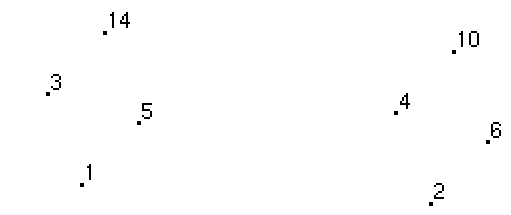
\includegraphics[width=\textwidth]{Images/Points.png}
    \caption{All Points}
  \end{subfigure}
  \begin{subfigure}[b]{0.35\textwidth}
    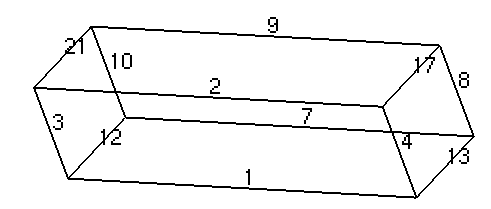
\includegraphics[width=\textwidth]{Images/Lines.png}
    \caption{All Lines}
  \end{subfigure}

  \begin{subfigure}[b]{0.35\textwidth}
    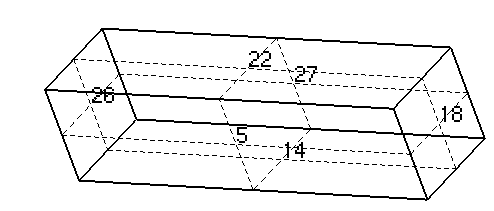
\includegraphics[width=\textwidth]{Images/Surface.png} 
    \caption{All Surface}
  \end{subfigure}
  \begin{subfigure}[b]{0.35\textwidth}
    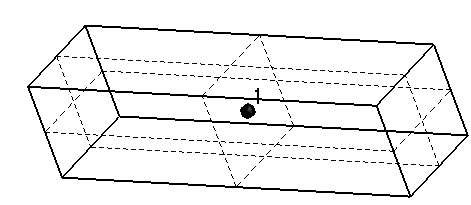
\includegraphics[width=\textwidth]{Images/Volume.png}
    \caption{All Volume}
  \end{subfigure}

 \caption{\label{Geometric-entities}  Showing  Geometrical
  Entities.  Every  point, line, surface and volume has an unique identification
  number assigned to it.}

\end{figure}

Figure~\ref{Geometric-entities}  shows,  the  different  unique identification
number  attached  to  each  of  the  nodes,  lines,  surface and volume of the
geometry of \textbf{cantilever beam}. The user can now \textbf{create physical
groups}  of  type  \textit{\{nodes, lines, surface, volume\}} containig one or
more  geometrical  entities  of  that type i.e. each is either \textit{points,
lines, nodes and surface} respectively. 

\paragraph{Physical  Groups}  are  groups of same type \textit{\{nodes, lines,
surface,  volume\}} of elementary geometrical entities. These \textbf{Physical
Groups}  cannot  be  modified  by  geometry commands. Their only purpose is to
assemble  elementary  entities  into  larger  groups, possibly modifying their
orientation,  so  that  they  can  be referred to by the mesh module as single
entities.  As  is  the  case  with  elementary entities, each \textit{physical
point, physical line, physical surface or physical volume} are also assigned a
unique identification number. 

\textbf{Note:- } A \textbf{geometrical entity} has only one elemenatry entity 
number but can be a part of many \textbf{physical groups} by sharing their 
\textit{identification number}.

Below is the continuation of \textbf{\textit{Example1.geo}} in \textbf{Gmsh} 
for creating \textbf{physical Groups} of \textit{cantilever beam}. Just for 
the sake of example, \textbf{4 physical Groups} are created which consisit 
of all points, lines, surface and volume respectively of the 
\textbf{cantilever beam model}.

\begin{lstlisting}[language=C,backgroundcolor=\color{grayish}]
$ vim Example1.geo 
.....
Physical Point ("All Points") ={1,2,3,4,5,6,10,14};
Physical Surface("All Surface group") = {5,14,22,27,18,26};
Physical Line("All Lines") ={1,2,3,4,12,13,21,17,7,8,9,10};
Physical Volume("All Volume") ={1};
\end{lstlisting}

\begin{figure}[h]

  \centering
  \begin{subfigure}[b]{0.35\textwidth}
    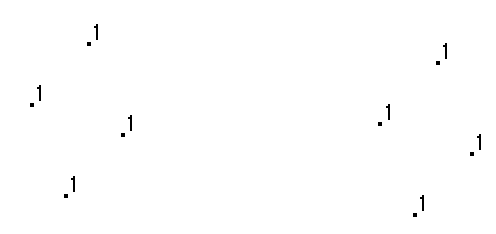
\includegraphics[width=\textwidth]{Images/PhysicalPoints.png}
    \caption{Physical group of Points}
  \end{subfigure}
  \begin{subfigure}[b]{0.35\textwidth}
    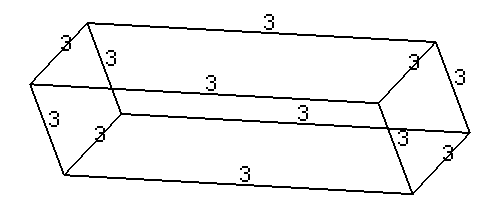
\includegraphics[width=\textwidth]{Images/PhysicalLines.png}
    \caption{Physical group of Lines}
  \end{subfigure}

   \begin{subfigure}[b]{0.35\textwidth}
    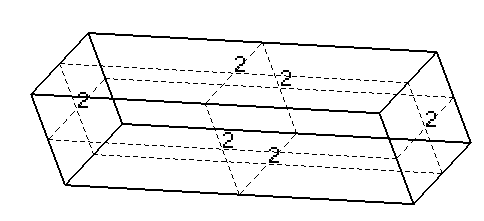
\includegraphics[width=\textwidth]{Images/PhysicalSurface.png} 
    \caption{Physical group of Surface}
  \end{subfigure}
  \begin{subfigure}[b]{0.35\textwidth}
    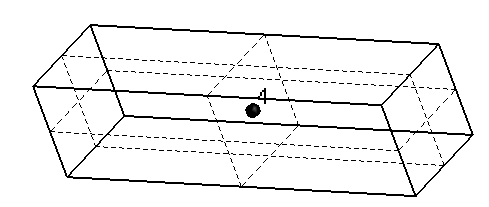
\includegraphics[width=\textwidth]{Images/PhysicalVolume.png}
  \caption{Physical group of Volume}
  \end{subfigure}

  \caption{\label{4-physical-groups} Showing all 4 Physical Groups with entities 
  numbered by their physical group id's}

\end{figure}

All   the   \textbf{geometrical  entities}  have  a  \textbf{tag  list}  which
\textbf{contains  the  ids of the \textbf{physical groups} to which it belongs
or  is  associated}.  In  the above example of Figure~\ref{4-physical-groups},
\textit{every  point,  line,  surface,  volume  } belongs to only one physical
group  and thus are showing only one associative number against themselves. In
Figure~\ref{multiple-physical-groups}   shows   \textbf{geometrical  entities}
which  are  \textit{part of many physical groups}. For example:- the volume in
the  figure  is  shown  to be a part of two \textbf{physical group of volumes}
\textit{having id 1 and 7}. 

\begin{figure}[h]
  \centering
  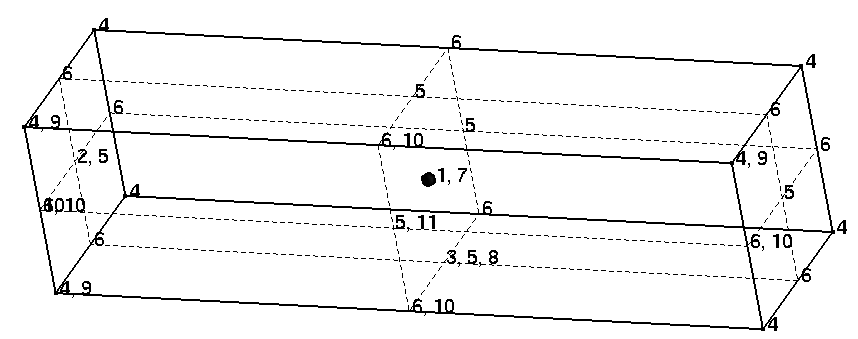
\includegraphics[scale=0.3]{Images/MultiplePhysicalGroups.png}
  \caption{\label{multiple-physical-groups} Showing geometrical entities associated 
  with more than one physical group}
\end{figure}

The whole idea of creating a \textbf{Physical Group} of \textit{points, lines,
surfaces  and  volumes}  and  giving it a unique string name is to allow quick
\textbf{identification  and  manupulation} during \textit{post-procESSIng}. In
\textbf{Gmsh}  the  name  of  these  \textbf{Physical  Group} along with their
corresponding  elements  and  nodes gets transferred to the mesh \textbf{.msh}
file   as   shown   below.   Later   in  Figure~\ref{gmsh-physical-group}  how
\textbf{Gmsh interpretes} these \textbf{Physical groups} in \textbf{.msh} file
is described.

\begin{lstlisting}[language=C]
$cat Example1.msh
.....
$PhysicalNames
4
0 1 "All Points"
1 3 "All Lines"
2 2 "All Surface group"
3 4 "All Volume"
$EndPhysicalNames
......
\end{lstlisting}

\textbf{Note:-   }   While   creating   a  \textbf{physical  group}  in  Gmsh,
\textbf{only the information (nodes and elements) of that physical group} gets
written  in  the  \textbf{.msh} file \textbf{and rest are not written}, so the
user  must  be  \emph{carefull  to create physical groups of all entities
which  he  needs  during post-processing}. More information about \textbf{Gmsh
syntaxing,  physical  groups,  commands,  .msh  file, save options ... etc} is
available            on           its           online           documentation
\url{http://geuz.org/gmsh/doc/texinfo/gmsh.html}

\begin{figure}[h]
  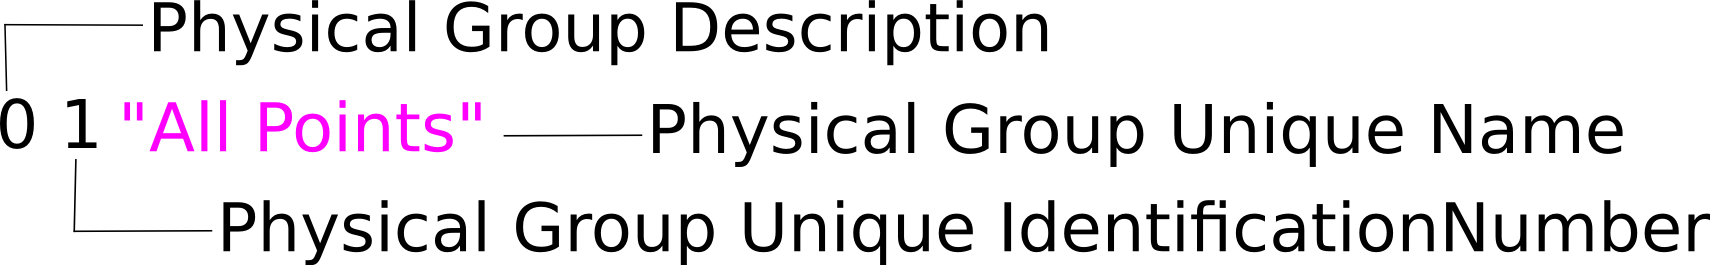
\includegraphics[scale=1.8]{Images/PhysicalDes.png}
  \centering
  \caption{\label{gmsh-physical-group} Description showing how gmsh interprets the Physical Groups.}
\end{figure}

\begin{itemize}

  \item[$\bullet$]  \textbf{Physical  Group  Description  ::  }  Gmsh uses it to
  identify  the  type  of  physical group. $0,1,2 and 3$ represents the physical
  group of geometric points, lines, surface and volume respectively.
  
  \item[$\bullet$]  \textbf{Physical  Group Unique Identification Number :: } It
  is  an  unique  identification  number automatically assigned to each physical
  group by gmsh.
  
  \item[$\bullet$]  \textbf{Physical  Group Unique Name :: } It is also the same
  as  \textit{Physical Group Unique Identification Number} but the difference is
  that  it  is not automatic but defined by the user and that too in the form of
  \textit{\textbf{string}}.

\end {itemize}

The gmESSI Translater utilizes the property of naming the physical group as
\textit{\textbf{string}} to get \textbf{gmESSI commands} from the user
\textbf{written as a part of the Physical group's name} and then operates on
the same physical group alongwith which the command was written to carry out the
translation to ESSI comands. Below in
\href{http://beta.sumeetsinha.in/gmESSI/Examples/Example1/Example1.geo}
{Example1} which is a \textit{Cantilever analysis}, it is shown how to
\textbf{create physical groups} with their \textbf{string name as gmESSI Syntax}
and then carry out translation with gmESSI translator using the \textbf{.msh}
file produced. Later in Figure~\ref{gmESSI-physical-group} how \textbf{gmESSI
translator interpretes} these \textbf{Physical groups} in \textbf{.msh} file is
described.

\begin{lstlisting}[language=C]
$ vim Example1.geo 
......
Physical Surface ("$FixedSurface$ [Add_All_Node{m,3}] [Fix{all}]") = {26}; 
Physical Line("$ApplyForce$ [Add_Node_Load_Linear{Fx,10*kN}]") ={8};  
Physical Volume("$CantileverVolume$ [Add_8NodeBrick{1}]") ={1};    
\end{lstlisting}

\begin{lstlisting}[language=C]
$cat Example1.msh
......
$PhysicalNames
3
1 2 "$ApplyForce$ [Add_Node_Load_Linear{Fx,10*kN}]"
2 1 "$FixedSurface$ [Add_All_Node{m,3}] [Fix{all}]"
3 3 "$CantileverVolume$ [Add_8NodeBrick{1}]"
$EndPhysicalNames
......
\end{lstlisting}

\begin{figure}[h]
  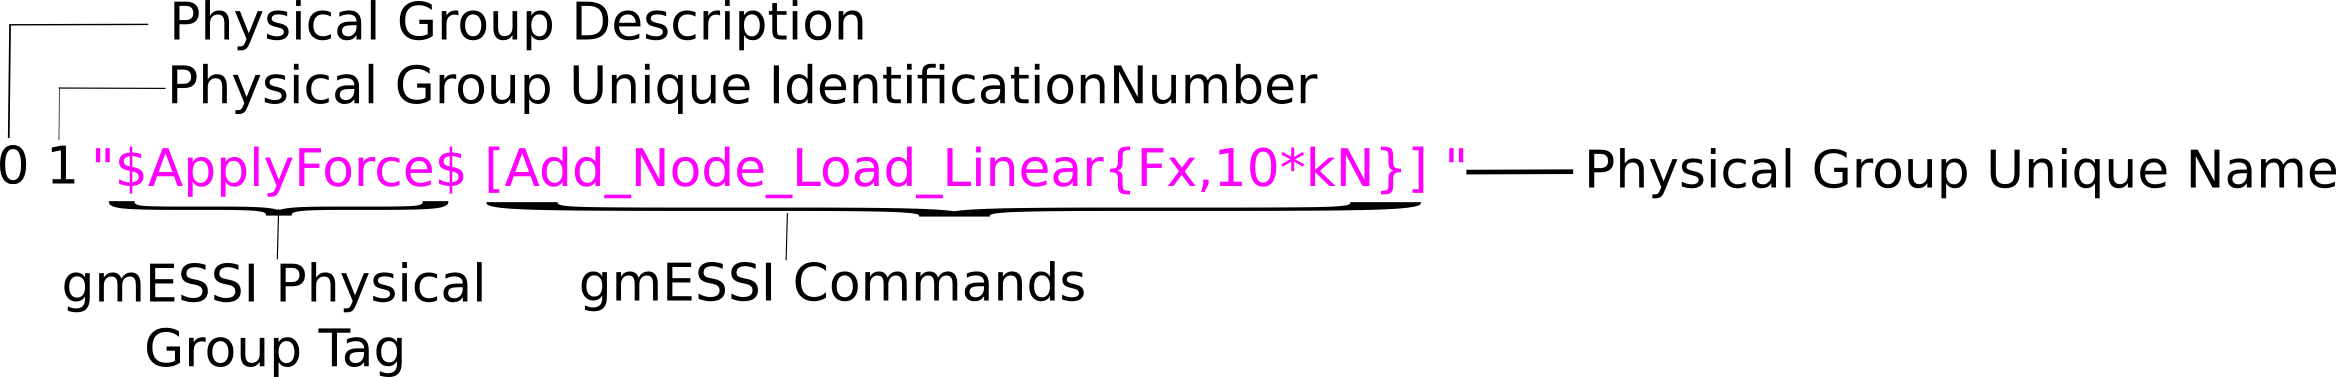
\includegraphics[scale=1.8]{Images/gmESSIPhysicalDes.png}
  \centering
  \caption{\label{gmESSI-physical-group} Description showing how gmESSI interprets the Physical Groups.}
\end{figure}

For gmESSI translator, the whole  \textbf{Physical Group Unique Name} is
basically a combination of two parts as shown below.

\begin{itemize}   

  \item[$\bullet$] \textbf{gmESSI Physical Group Tag :: } As
  name describes it a tag given to the physical group by the user. It should be
  quoted between \textbf{\$} signs. It is just for the user reference to have a
  description about the physical group.   

  \item[$\bullet$] \textbf{gmESSI
  Commands :: } It is a list of commands that gmESSI translator understands.
  Each command is quoted between \textcolor{violet}{\textbf{[ ]}}.
  \textit{Multiple commands are separated by space}. 

\end {itemize}

The gmESSI translator reads the command
\textcolor{violet}{\textit{\textbf{[Add\_Node\_Load\_Linear\{Fx,10*kN\}]}}}
and applies nodal force $\textbf{Fx=10*kN}$ to all the nodes of the physical
group i.e (id $\textbf{2}$ or \textbf{ApplyForce}) alongwith which the command
was written.

\textbf{Note:- } For textit{textbf{Gmsh}}
\textcolor{violet}{textbf{"$ApplyForce$ [Add_Node_Load_Linear{Fx,10*kN}]"}} is
nothing but a name for the Physical group having id $2$. Whereas, for
\textit{textbf{gmESSI}} its a command for textit{adding uniform nodal load} to
that physical group.


%%%%%%%%%%%%%%%%%%%%%%%%%%%%%%%%%%%%%%%%%%%%%%%%%%%%%%%%%%%%%%%%%%%%%%%%%%%%%%%
\section{gmESSI Syntax}

gmESSI Translator as said above utilizes the \textbf{naming of the physical
groups} to get commands from the user and \textit{\textbf{carry out the
converion by acting on the same physical group elements and nodes}}.

%%%%%%%%%%%%%%%%%%%%%%%%%%%%%%%%%%%%%%%%%%%%%%%%%%%%%%%%%%%%%%%%%%%%%%%%%%%%%%%
\subsection{gmESSI Syntax}

gmESSI follows strict syntax. gmESSI parses the \textbf{physical group name
string} to find out the command, so \textit{sticking to the syntax is very
important} for it to understand the commands. Let us have a quick look at the
syntax

%%%%%%%%%%%%%%%%%%%%%%%%%%%%%%%%%%%%%%%%%%%%%%%%%%%%%%%%%%%%%%%%%%%%%%%%%%%%%%%
\subsubsection{Physical Group Names}

Physical group names for gmESSI can follow two situations as described below

\begin{itemize}

  \item[$\bullet$] \textbf{Only Physical Group Tag with no commands ::} 
  As the name describes it referes to the situation in which, the user is only 
  interested to make physical group for its convinience but do not need to have 
  an gmESSI command associated with it for conversion. In that case the user  
  can follow two syntax either\\    
  \centerline {\textcolor{violet}{"\$Physical Group Tag\$"} or 
  \textcolor{violet}{"Physical Group Tag"}}

  \item[$\bullet$] \textbf{Physical Group Tag with commands ::} When the user
  wants gmESSI command/s associated with the physical group for convesion,    in
  that case the syantax is \\ 

  \centerline {\textcolor{violet}{"\$Physical
  Group Tag\$ [Command1\{arg1,arg2\}]  [Command2\{arg1,arg2,arg3\}]"}}

  \centerline{\sout{\textcolor{violet}{"Physical Group Tag
  [Command1\{arg1,arg2\}]  [Command2\{arg1,arg2,arg3\}]"}}} 

\end {itemize}

%%%%%%%%%%%%%%%%%%%%%%%%%%%%%%%%%%%%%%%%%%%%%%%%%%%%%%%%%%%%%%%%%%%%%%%%%%%%%%%
\subsubsection{Physical Group Tags Syntax}

Physical  group tags can be any alphanumeric sequence but should not contain any
of  these  \textcolor{violet}{[  ]\$} literals in their names. The tags can have
any spaces in between and must be enclod between \textcolor{violet}{\textbf{\$}} sign.\\
\centerline       {\textcolor{violet}{"\$Physical       Group      Tag1\$"      
"\$PhysicalGroupTag2\$"}                 \rcancel{\textcolor{violet}{"\$Physical
\$GroupTag3\$"}}}

\centerline{\rcancel{\textcolor{violet}{"\$Physical              [GroupTag3\$"}}
\textcolor{violet}{"\$Physical\_Group\_Tag3\$"}
\rcancel{\textcolor{violet}{"\$Physical GroupTag3"}}}

%%%%%%%%%%%%%%%%%%%%%%%%%%%%%%%%%%%%%%%%%%%%%%%%%%%%%%%%%%%%%%%%%%%%%%%%%%%%%%%
\subsubsection{gmESSI Command Syntax}

gmESSI translator commands are always enclosed between opening/closing square brackets 
\textbf{\textcolor{violet}{[}} and \textbf{\textcolor{violet}{]}} respectively. 
A typical gmESSI command syntax is shown in Figure~\ref{gmESSI-command}

\begin{figure}[h]
  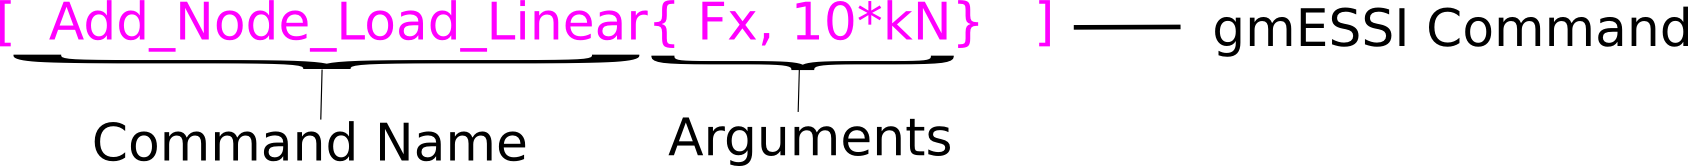
\includegraphics[scale=1.8]{Images/gmESSICommandSyntax.png}
  \centering
  \caption{\label{gmESSI-command} gmESSI command description}
\end{figure}

\begin{itemize}

  \item[$\bullet$] \textbf{Command Name :: } Just as regular function gmESSI
  Commands have a name and take arguments. The names are usually self
  explanatory of its function like
  \textcolor{violet}{\textit{Add\_8NodeBrick\{material\}, Free\{dof\},
  Var\{variable,value\} .. etc}}

  \item[$\bullet$] \textbf{Arguments :: } Arguments as always are separated by
  \textbf{comma} \textcolor{violet}{\textbf{','}}.  

  \begin{itemize}

    \item[$\bullet$]  The arguments of gmESSI commands can also have tags associated 
    with them so that it becomes easy for the user to interpret the argument and 
    make changes in future. The tag and the argument is separaed by \textcolor{violet}
    {\textbf{:=}}. Tag itself has no meaning but it serves as an important information 
    center for user. An example is shown below to show how tags are applied.\\

    $-$ gmESSI command having arguments without tags
    \begin{enumerate}
       \item  \textcolor{violet}{[Add\_Node\_Load\_Linear\{Fx,10*kN\}]}    
    \end{enumerate}

    $-$ gmESSI command having arguments with tags
    \begin{enumerate}
       \item  \textcolor{violet}{[Add\_Node\_Load\_Linear\{ direction:= Fx, magnitude:= 10*kN\}]}    
       \item  \textcolor{violet}{[Add\_Node\_Load\_Linear\{ direction:= Fx, 10*kN\}]}      
       \item  \textcolor{violet}{[Add\_Node\_Load\_Linear\{ Force_Direction:= Fx, Strength:=10*kN\}]}
    \end{enumerate}

   
   It can be seen from above examples that the tags are optional and also the user 
   can put their own tag names. The sublime plugin 
   \href{https://packagecontrol.io/packages/gmESSI-gmsh%20tools}
   {\textbf{gmESSI-gmsh Tools}} comes
   with elaborative tags for the parameters and a lot more syntax-colouring and 
   text-completionfor gmESSI commands. Users are encouraged to use the plugin 
   and take its advantage. \\

    \item[$\bullet$]  Most  of the time these \textbf{arguments are dummy} which
    means that they just get copied to their \textbf{equivalent ESSI command} at
    \textit{their    respective   places}.   These   arguments   thus   have   a
    \textbf{string}       datatype.      For      example:      the      command
    \textcolor{violet}{Add\_Node\_Load\_Linear\{Fx,10*kN\}} is equivalent to the
    ESSI  command  \textcolor{violet}{add load \#\{\} to node \#\{\} type linear
    \{\}  =  \{\}}. \textcolor{violet}{Fx} and \textcolor{violet}{10*kN} goes to
    their  respective  position  directly through the translater as shown in the
    Figure~\ref{gmESSI-conversion}  \textbf{Load number \textcolor{blue}{1}} and
    \textbf{node number \textcolor{blue}{32}} are computed by the translator and
    then inserted in the ESSI command.

    \begin{figure}[!h]
      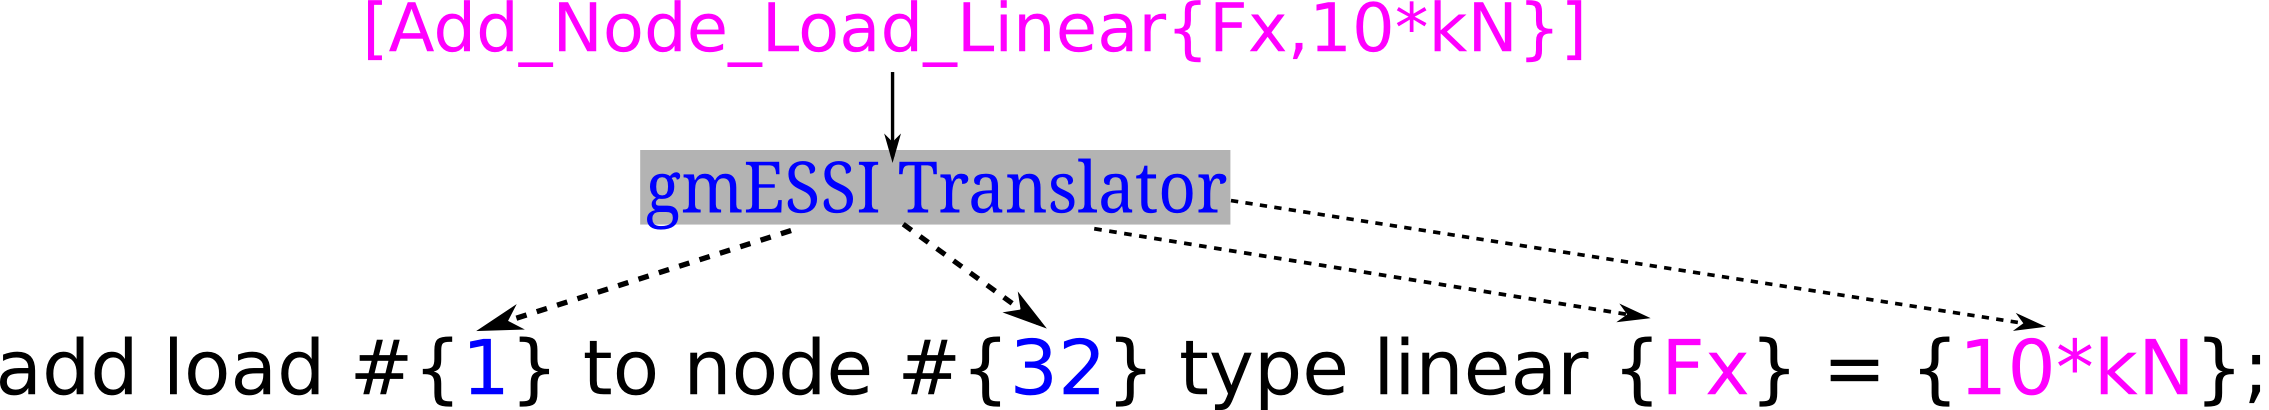
\includegraphics[width=10cm]{Images/gmESSIArguments.png}
      \centering
      \caption{\label{gmESSI-conversion} gmESSI conversion description}
    \end{figure}

    \textbf{Note:-}  gmESSI Translator \textit{does not provide syntax checking}
    for  \textbf{those  dummy  arguments}.  It means that, whatever you write it
    gets  copied  at  the respective position in the equivalent ESSI command, so
    the user must be carefull with what they are writing in these arguments. For
    Example                   :-                   the                   command
    \textcolor{violet}{Add\_Node\_Load\_Linear\{ ForceDirection, Magnitude\}}    
    based on the arguments can get converted to


    \begin{enumerate}

       \item      {\textcolor{violet}{Add\_Node\_Load\_Linear\{Fx,10*kN\}}  $-->$
       \textcolor{violet}{add load \#1 to node \#32 type linear Fx = 10*kN}}
       
       \item   {\textcolor{violet}{Add\_Node\_Load\_Linear\{Fx,10\}}        $-->$
       \textcolor{violet}{add load \#1 to node \#32 type linear Fx = 10}}
       
       \item      {\textcolor{violet}{Add\_Node\_Load\_Linear\{ft,10*kN\}}  $-->$
       \textcolor{violet}{add load \#1 to node \#32 type linear ft = 10*kN}}

    \end{enumerate}

    All the above conversions are correct. But conversion \textbf{1)} is correct
    for    \textbf{ESSI}    because    \textbf{ForceDirection}    is    one   of
    \textit{Fx,Fy,Fz}  and  \textbf{Magnitude} \textbf{10*kN} has \textit{proper
    units}. \emph{So the user must be very careful with what they are writing in
    the arguments}.\\

    \item[$\bullet$] Some of the arguments \textit{are not string but
    represent numerical quantities}, which are manupulated by the translator
    during conversion. Thus, the user must supply only numbers as strings without
    any alphabets else it would lead an unexpected termination of program. These
    arguments corresponds to \textbf{Special Commands} such as
    \textcolor{violet}{Connect Command} and \textcolor{violet}{Material
    Variational Commands}. The manual talks about them later.   

  \end {itemize}

\end {itemize}

%%%%%%%%%%%%%%%%%%%%%%%%%%%%%%%%%%%%%%%%%%%%%%%%%%%%%%%%%%%%%%%%%%%%%%%%%%%%%%%
\subsection{Command's Physical/Entities Group}

As stated somewhere else, \textbf{gmESSI commands} operates on \textit{
physical groups}. \textit{The physical groups} on which it operates is the
one alongwith which the command is written. But \textbf{gmESSI} provides a
more flexible approach for these commands so \textit{that they can be
written anywhere and can \textbf{operate on any Physical group as well as
Entity group}}. Let us look at them one by one

\begin{itemize}

  \item[$\bullet$]  \textbf{Default  Physical Group to gmESSI Commands ::} The
  default physical group on which the gmESSI commands operate is the one along
  with  which  it  is written in the \textbf{.msh} file. Let's look at some of
  them

  \begin{itemize}

    \item           {1           2          \textcolor{violet}{"\$ApplyForce\$
    [Add\_Node\_Load\_Linear\{Fx,10*kN\}]"} operates on physical group 2 }
    
    \item           {3           5          \textcolor{violet}{"\$ApplyForce\$
    [Add\_8NodeBrick\{material\#1\}]"} operates on physical group 5 }

  \end{itemize}

  \item[$\bullet$]  \textbf{Userdefined  Physical  and  Entity Group to gmESSI
  Commands  ::}  The flexibility of gmESSI syntax allows the users to operates
  it's  command  on  specific physical groups or geometric entities. This user
  specifies    the    group    by    including    an    additional    argument
  \textcolor{violet}{Physical_group/Entity_Group\#Tag}  in front of the gmESSI
  commands   describing   the   group.   The   \textbf{tag}   can   be  either
  \textit{Physical\_Group\_Id,  Physical\_Group\_Name}. Let's  look at some of
  them

  \begin{itemize}

    \item {1         2         \textcolor{violet}{"\$ApplyForce\$         [
    Add\_Node\_Load\_Linear\{Physical\_Group\#3,Fx,10*kN\}]"}     operates    on
   physical group 3}

    \item {1         2         \textcolor{violet}{"\$ApplyForce\$         [
    Add\_Node\_Load\_Linear\{Entity\_Group\#5,Fx,10*kN\}]"}  operates  on entity
   gr oup 5}

    \item {3         5         \textcolor{violet}{"\$ApplyForce\$         [
    Add\_8NodeBrick\{Entity\_Group\#9,1\}]"} operates on entity group 9}

    \item {3    5   \textcolor{violet}{"\$ApplyForce\$   [
    Add\_8NodeBrick\{Physical\_Group\#CantileverVolume,       1\}]       "}}   
    {operates    on    physical    group   which   has   string\_tag   as
    CantileverVolume.}  


  \end{itemize}

  For          example          in          reference        to    {Example1.msh
  Physical\_Group\#CantileverVolume   or   Physical\_Group\#3   refers  the  same
  physical group}
 
  A  \textbf{Entity  group}  is the same as \textbf{Physical group} but
  contains  all  the  geometrical  entities  that  have  the same unique id. While
  \textbf{Physical  group}  contains  many  geometrical  entities  but of only one
  entity  type, \textbf{Entity group} can contain \textbf{mixture of entity types}
  but  \textbf{for  each  type maximum upto one geometrical entity}. For example:-
  \textcolor{violet}{Entity\_Group\#5}     contains     \textit{all    elemenntary
  geometrical  nodes,  lines,  surface  and  volumes  that have unique id as 5 and
  \textbf{are  present in mesh generated .msh} file}. In Figure 1 \textit{Point 1,
  Line 1 and Volume 1} belongs to \textbf{Entity Group} having id $1$.

  Whereas a \textbf{physical group} is a group of point, line, surface or
  volume defined by the user which contains all the geometrical entities that
  falls under that domain/group. Figure~\ref{4-physical-groups} shows physical groups.

  \textbf{Note:- } When the user \textit{explicitly} defines a
  \textit{physical/entity group} for the command, the command now \textbf{can
  be written anywhere} alongwith any physical group in the \textbf{.msh}
  file.

  \textbf{Note:- } Whenever one is applying an \textbf{General Elemental
  Command} or \textbf{Nodal Command} on an \textbf{entity group}, the user should be
  very carefully beacuse it might contain nodes from different elements and
  more than 1 type of elements respectively. Typically, when the meshes are
  created by gmsh automatically, the chances of this kind of conflicts are
  very less. But still user must be carefull while using Entity Group.

\end {itemize}

%%%%%%%%%%%%%%%%%%%%%%%%%%%%%%%%%%%%%%%%%%%%%%%%%%%%%%%%%%%%%%%%%%%%%%%%%%%%%%%
\section{gmESSI Output}

gmESSI Translator translates the commands of \textbf{.msh} file to different
\textbf{.fei} files and put them in a folder. It also updates the mesh
\textbf{.msh} file and puts it in the same folder. The \textbf{log of
translation, errors and warnings} are displayed on the terminal. Let us
demostrate each of them one by one using \textbf{Example1.msh}  and a
\textit{general meshfile name} \textbf{XYZ.msh}.

%%%%%%%%%%%%%%%%%%%%%%%%%%%%%%%%%%%%%%%%%%%%%%%%%%%%%%%%%%%%%%%%%%%%%%%%%%%%%%%
  \subsection{Folder \textcolor{blue}{\textit{XYZ\_ESSI\_Simulation}}}


    gmESSI Translator creates a folder at the place of execution. All the
    files are written in that folder only. Typically the name of the folder
    created for \textbf{XYZ.msh} file is
    \textcolor{blue}{XYZ\_ESSI\_Simulation}. In case the folder allready
    exists a \textcolor{brown}{warning message} is shown on the terminal.

    \begin{lstlisting}[language=C,backgroundcolor=\color{grayish}]
    $ gmESSI Example1.msh 

    <@\textcolor{blue}{Files will be converted to Example/Example1\_ESSI\_Simulation}@>  

    <@\textcolor{brown}{WARNING::Directory Allready Present. The contents of the Folder may get changed}@> 

    <@\textcolor{blue}{Files converted to Example/Example1\_ESSI\_Simulation}@>  
    \end{lstlisting}

    \textbf{By default the translation is allways done in the overwrite mode}
    meaning the previous existing files/folder if any would get changed and
    updated. But the user can turn off the mode by \textbf{non-overwrite
    mode} option \textcolor{violet}{\textbf{-o}} to create a new non-conflicting 
    folder \textcolor{blue}{XYZ\_ESSI\_Simulation\_n} where n
    refers to 1,2,3,...

    \begin{lstlisting}[language=C,backgroundcolor=\color{grayish}]
    $ gmESSI -o Example1.msh 

    <@\textcolor{blue}{Files converted to Example/Example1\_ESSI\_Simulation\_1}@>  
    \end{lstlisting}

      The execution of \textcolor{violet}{gmESSI XYZ.msh} produces warnings/errors in the following situtaions. 

    \begin{itemize}

      \item[$\bullet$] \textcolor{red}{ERROR:: Please Enter the Gmsh File ::}
        It occurs if the user does not give a filename. The possible situtaion
        for getting this error is \textcolor{violet}{gmESSI} and
        \textcolor{violet}{gmESSI -o XYZ.msh}

      \item[$\bullet$] \textcolor{red}{ERROR:: The program failed to open the
        file XYZ.msh } It occurs \textit{if the given file or one of the files
        in the argument does not exist or fails to open} because of some
        reason. Examples:- \textcolor{violet}{gmESSI Xyz.msh} and
        \textcolor{violet}{gmESSI - XYZ.msh}.

      \item[$\bullet$] \textcolor{brown}{WARNING::Directory Allready Present.
        The contents of the Folder may get changed ::} It occurs \textit{when
        users translates its file XYZ.msh in overwrite mode and the
        corresponding folder XYZ\_ESSI\_Simulation allready exists at the
        execution location}.

      \item[$\bullet$] \textcolor{blue}{Files converted to
        Example/Example1\_ESSI\_Simulation :: } The message refers to the
        location of the folder where the translations have been saved.

    \end{itemize}

%%%%%%%%%%%%%%%%%%%%%%%%%%%%%%%%%%%%%%%%%%%%%%%%%%%%%%%%%%%%%%%%%%%%%%%%%%%%%%%
\subsection{Translation Log \textcolor{blue}{\textit{Terminal}}}


gmESSI Translator displays the log of translation of \textbf{gmESSI
commands} to \textbf{ESSI commands} on the terminal. Proper
\textcolor{red}{Errors Messages} and \textcolor{brown}{Warnings} are
\textbf{echoed} to the user. The \textbf{execution of the commands} are
\textbf{sequential} which means the commands written first are executed
first and similarly their success and failure is also echoed first. Let us
look at this aspect with Example1.msh.

\begin{lstlisting}[language=C]
$cat Example1.msh
......
$PhysicalNames
3
1 2 "$ApplyForce$ [Add_Node_Load_Linear{Fx,10*kN}]"
2 1 "$FixedSurface$ [Add_All_Node{m,3}] [Fix{all}]"
3 3 "$CantileverVolume$ [Add_8NodeBrick{1}]"
$EndPhysicalNames
......
\end{lstlisting}

Here,     the     sequence     of     execution     of     commands     is
\textcolor{violet}{[Add\_Node\_Load\_Linear\{Fx,10*kN\}]}                ,
\textcolor{violet}{[Add\_All\_Node\{m,3\}]}                              ,
\textcolor{violet}{[Fix\{all\}]}                                       and
\textcolor{violet}{[Add\_8NodeBrick\{1\}]}.  Notice  that  the  same order
gets reflected in the translation log on the terminal as shown below.

\begin{lstlisting}[language=C,backgroundcolor=\color{grayish}]
$ gmessi ./Example1.msh
......
Add_Node_Load_Linear{Fx,10*kN}         Found!!        Sucessfully Converted
Add_All_Node{m,3}                      Found!!        Sucessfully Converted
Fix{all}                               Found!!        Sucessfully Converted
Add_8NodeBrick{1}                      Found!!        Sucessfully Converted
......
\end{lstlisting}

Apart from the \textbf{translation log details} on the terminal in the front of user, similar kind of log gets added for each translation of \textbf{gmESSI commands} in their respective files in which they are translated.    
In these files \textbf{each sucessfull translation} is enclosed between corresponding \textbf{RespectiveUserCommand Begins} and \textbf{RespectiveUserCommand Ends}. The same is shown below through the contents of Example1\_geometry.fei. Notice that all the translations are enclosed between \textbf{Begins and Ends Tag}.   

\begin{lstlisting}[language=C]
$ cat Example1_geometry.fei
//****************************************************************
//              AddAllNode{m,3}Begins
//****************************************************************

add node # 1 at (0.000000*m ,0.000000*m ,0.000000*m ) with 3 dofs;         
add node # 2 at (1.000000*m ,0.000000*m ,0.000000*m ) with 3 dofs;         
add node # 3 at (0.000000*m ,1.000000*m ,0.000000*m ) with 3 dofs;                     
..................................................................

//****************************************************************
//              AddAllNode{m,3}Ends
//**************************************************************** 
\end{lstlisting}

\textbf{Note:- } The textbf{textit{ordering/sequence of commands in ESSI
analysis file is important}} and so the user must make sure that the
translations are made in the same order or if not the user should change it
\textbf{manually by (cut/copy/paste)} in textbf{geometry.fei, load.fei and
analysis.fei} files before execution.


Having given a short descripton of the Translation log, let us look more
closely one by one and understand the \textcolor{blue}{messages},
\textcolor{red}{errors} and \textcolor{brown}{warnings} promted in the log on
the terminal.

\begin{itemize}

  \item[$\bullet$] \textcolor{blue}{Found!! ::} 
  This message in front of the
  gmESSI  command  as  shown  above on translation log in the terminal means
  that,  \textit{the  corresponding  command was found in the \textbf{gmESSI
  Command Library}}.
  
  \item[$\bullet$]   \textcolor{blue}{  Sucessfully  Converted  ::}  
  As  the
  message  itself  describes,  it  occurs  \textit{if  the  command has been
  sucessfully translated}.
  
  \item[$\bullet$]  \textcolor{red}{Not  Found!! ::} 
  It occurs if the gmESSI
  Translator  \textit{could  not  find  the  arbitraty  command  XYZ  in the
  \textbf{gmESSI  Command  library}}.  Example:- \textbf{Loading\{Fx,10*kN\}
  \textcolor{red}{NotFound!!}}
  
  \item[$\bullet$]  \textcolor{brown}{WARNING::  Execuation  of  the command
  escaped. The Gssi command XYZ could not be found ::} 
  The gmESSI Translator
  does  not  terminate  the  translation  if a command is not found, instead
  gives  this  warning  message  following  the  \textcolor{red}{Not Found!!
  Error}.
  
  \item[$\bullet$] \textcolor{red}{Error:: The command XYZ has a syntaxERROR
  in  Entity\_Group/Physical\_Group\# tag ::} 
  It occurs if there is a syntax error in
  \textcolor{violet}{Entity\_Group/Physical\_Group\#}     argument.    The    correct
  represention    for   \textbf{Physical   and   Entity   group   Tags}   is
  \textcolor{violet}{Physical\_Group\#n}                                 and
  \textcolor{violet}{Entity\_Group\#n}          respectively,          where
  \textcolor{violet}{n}  is  the  \textbf{group  id  as 1,2,3..}. Example of
  improper     representation     are    \textcolor{red}{Phy\#2,
  Physical\#2, Ent\#2, Entiti\#2 ..}
  
  \item[$\bullet$]  \textcolor{brown}{Warning::  The  command  XYZ failed to
  convert  as there is no such Physical/Entity Group ::} 
  It occurs if one of
  the arguments in the command is \textcolor{violet}{Enty/Physical\_Group\#}
  and  \textit{the  specified  entity or physical group by the user does not
  exists in the \textbf{.msh} file}.
  
  \item[$\bullet$]  \textcolor{brown}{Warning::  The  command  XYZ could not
  find any nodes/elements on which it operates :: } 
  It occurs \textit{if for
  a  specified command, the required element types for translation could not
  be   found   in  the  specified  Physical/Entity  group.}  For  Examples:-
  \textcolor{violet}{[8NodeBrick\{Physical\_Group\#1,1\}]}  would  give this
  \textcolor{brown}{warning}  as  the \textcolor{violet}{Physical\_Group\#1}
  being  a  Physical  line  group \textbf{does not contain any 8-Noded Brick
  elements on which this command operates}.
  
  \item[$\bullet$]  \textcolor{red}{ERROR:: Gmsh File has invalid symbols in
  Node  Section.  Unable  to  convert string to integer in Gmsh File :: } 
  It
  occurs  \textit{if  there  is perhaps a string inside the Nodes section of
  \textbf{.msh} file}.
  
  \item[$\bullet$]  \textcolor{red}{ERROR::  The  command  XYZ  has a syntax
  errors :: } 
  It occurs \textit{if the specified command by the user contain
  any stntax errors caught while parsing the command}.
  
  \item[$\bullet$]  \textcolor{red}{ERROR:: Gmsh File has invalid symbols in
  Element  Section. Unable to convert string to integer in Gmsh File :: } 
  It occurs  \textit{if there is perhaps a string inside the Element section of
  \textbf{.msh} file}.

\end{itemize}

%%%%%%%%%%%%%%%%%%%%%%%%%%%%%%%%%%%%%%%%%%%%%%%%%%%%%%%%%%%%%%%%%%%%%%%%%%%%%%%
\subsection{Geometric File \textcolor{blue}{\textit{XYZ\_geometry.fei}}}

\textbf{Geometric file} \textit{XYZ\_geometric.fei} is one of three parts of
ESSI Analysis file and it contains the translation of commands related to the
geometry of the structure, like \textbf{\textit{declaration of nodes and elements}}.

%%%%%%%%%%%%%%%%%%%%%%%%%%%%%%%%%%%%%%%%%%%%%%%%%%%%%%%%%%%%%%%%%%%%%%%%%%%%%%%
\subsection{Load File \textcolor{blue}{\textit{XYZ\_load.fei}}}

\paragraph{Load   file}  \textit{XYZ\_load.fei}  contains  the  translation  of
commands  related to the load and boundary conditions on the structure, like
\textbf{\textit{declaration  of fixities, boundary conditions, master slave,
nodal loads, surface loads etc...}}.

%%%%%%%%%%%%%%%%%%%%%%%%%%%%%%%%%%%%%%%%%%%%%%%%%%%%%%%%%%%%%%%%%%%%%%%%%%%%%%%
\subsection{Analysis File \textcolor{blue}{\textit{XYZ\_analysis.fei}}}

\textbf{Analysis file} textit{XYZ_analysis.fei} is the main file which is run
on ESSI. The main file textbf{textit{includes load file and geometry file}}
through textbf{include command}. A typical analysis file after conversion
looks like the following.

\begin{lstlisting}[language=C]
$ cat Example1_analysis.fei

  model name "Example1.msh";

  include "/Examples/Example1_ESSI_Simulation/Example1_geometry.fei";

  new loading stage "Stage_1 Loading";

  include "/Examples/Example1_ESSI_Simulation/Example1_load.fei";

\end{lstlisting}

The user can now \textcolor{violet}{add solver, time steps and even rearrange}
the file structure accordingly to \textbf{ESSI synatx}.
{\textcolor{red}{Please not that \textit{ESSI Interpreter} is sequential and
\textit{follows certain ordering in commands}, \textbf{like materials should
be declared before assigning to elements, master-slave can be assigned only
when both nodes are declared .. etc.}. The user should be carefull with the
order in which conversions are made and if necessary should \textbf{change it
manually by (cut/copy/paste)} later in the \textbf{files geometry.fei,
load.fei and analysis.fei} or use the python module discussed later before
running in ESSI.}} \textcolor{blue}{{Please refer to the ESSI manual for more
details on the ordering of the commands.}}

%%%%%%%%%%%%%%%%%%%%%%%%%%%%%%%%%%%%%%%%%%%%%%%%%%%%%%%%%%%%%%%%%%%%%%%%%%%%%%%
\subsection{Mesh File \textcolor{blue}{\textit{XYZ.msh}}}

\textbf{Mesh file} textit{XYZ.msh} for most of times is the input XYZ.msh
file. But if textbf{textcolor{violet}{Connect Command}} is used, the file
contains textbf{textit{additional physical group, nodes and 2-noded
elements}}. The textbf{textcolor{violet}{Connect Command}} is discussed in
the more detail later in this manual.

%%%%%%%%%%%%%%%%%%%%%%%%%%%%%%%%%%%%%%%%%%%%%%%%%%%%%%%%%%%%%%%%%%%%%%%%%%%%%%%
\subsection{Updated ESSI Tags \textcolor{blue}{\textit{Terminal}}}

\textbf{Updated ESSI Tags} refers to the new Tag numbering reference
associated with ESSI Tags. textbf{ESSI} has tag numberings associated for
\textcolor{blue}{damping, displacement, element, field, load, material, motion
and node/nodes}. For example in textbf{ESSI Command}
\textbf{textcolor{violet}{add node \# 1  at (x,y,z)  with 3 dofs}},
\textbf{node} is an textbf{Tag} and requires a new number textit{ike 1 to be
associated with that node}. textbf{gmESSI translator} displays the textit{new
numberings available for each ESSI Tag} so that the user is made aware of new
numberings while manually specifying an ESSI command after the translation.

\begin{lstlisting}[language=C]
$ gmessi Example1.msh
  .....................
 <@\textcolor{blue}{******* Updated New Tag Numberring ********}@>
 <@\textcolor{blue}{damping         = 1}@>
 <@\textcolor{blue}{displacement    = 1}@>
 <@\textcolor{blue}{element         = 27}@>
 <@\textcolor{blue}{field           = 1}@>
 <@\textcolor{blue}{load            = 4}@>
 <@\textcolor{blue}{material        = 2}@>
 <@\textcolor{blue}{motion          = 1}@>
 <@\textcolor{blue}{node            = 55}@>
 <@\textcolor{blue}{nodes           = 55}@>

\end{lstlisting}
 
%%%%%%%%%%%%%%%%%%%%%%%%%%%%%%%%%%%%%%%%%%%%%%%%%%%%%%%%%%%%%%%%%%%%%%%%%%%%%%%
\section{gmESSI Commands Library}

Having the knowledge about the syntax, output files, errors and warnings, its
time to move on to different types of commands that gmESSI offers.
\textbf{gmESSI Translator} offers conversion for all the commands of
\textbf{ESSI}. \textit{The equivalent ESSI command to which gmESSI command
translates is also shown in forthcomming sections}. Apart from that there are
some special command that gmESSI supports. Just for simplicity  the commands
are categorised on \textit{the basis of their operation on nodes/elemnts}. As
stated earlier, the commands are translated to one of three file
\textbf{XYZ\_geometry.fei, XYZ\_load.fei and XYZ\_analysis.fei}. Let us look
at them closely one by one alongwith all its supported commands.

%%%%%%%%%%%%%%%%%%%%%%%%%%%%%%%%%%%%%%%%%%%%%%%%%%%%%%%%%%%%%%%%%%%%%%%%%%%%%%%
\subsection{Nodal Commands}


\textbf{Nodal commands} operates on all the textit{nodes of a physical/entity
group}. Their translations are written in \textbf{XYZ\_load.fei} file. For
example:- \textcolor{violet}{[Fix{Physical\_Group\#1,ux}]} would
\textcolor{violet}{fix ux} dof of all the nodes of physical group 1. The
different commands under this category and their corresponding ESSI commands
are

\begin{itemize}

  \item \textcolor{violet}{gmESSI :: [Add\_Node\_Mass\{mx,my,mz\}]}\\
  \textbf{Esssi :: add mass to node \#\{\} mx =\{\} my =\{\} mz =\{\}}\\
  Description :: \textit{add mass to node \# $<.>$ mx = $<mass>$ my = $<mass>$
  mz = $<mass>$}

  \item \textcolor{violet}{gmESSI :: [Add\_Node\_Mass\{mx,my,mz,Imx,Imy,Imz\}]} \\ 
  \textbf{Esssi :: add mass to node \#\{\} mx =\{\} my =\{\} mz =\{\} Imx =\{\} Imy =\{\} Imz
  =\{\}}\\   Description :: \textit{add mass to node \# $<.>$ mx = $<mass>$ my =
  $<mass>$ mz = $<mass>$ Imz = $<mass*length^2>$ Imy = $<mass*length^2>$ Imz =
  $<mass*length^2>$}

  \item \textcolor{violet}{ gmESSI :: [Add\_Node\_Damping\{damping\_no\}]}\\
  \textbf{ ESSI :: add damping \#\{\} to node \#\{\}}\\
  Description :: \textit{add damping \# $<.>$ to node \# $<.>$}

  \item \textcolor{violet}{ gmESSI :: [Fix\{dofs\}]}\\
  \textbf{ ESSI :: fix node \#\{\} dofs \{\}}\\
  Description :: \textit{add damping \# $<.>$ to node \# $<.>$}

  \item \textcolor{violet}{ gmESSI :: [Free\{dofs\}]}\\
  \textbf{ ESSI :: free node \#\{\} dofs \{\}}\\
  Description :: \textit{free node \# $<.>$ dofs $<.>$}

  \item \textcolor{violet}{ gmESSI :: [Add\_Master\_Slave\{master\_node, dof\}]}\\
  \textbf{ ESSI :: add constraint equal dof with master node \#\{\} and slave node \#\{\}  dof to constrain \{\}}\\
  Description :: \textit{add constraint equal dof with master node \# $<.>$ and slave node \# $<.>$ dof to constrain $<.>$}

  \item \textcolor{violet}{ gmESSI :: [Remove\_Master\_Slave\{\}]}\\
  \textbf{ ESSI :: remove constraint equal dof node \#\{\} }\\
  Description :: \textit{remove constraint equaldof node \# $<.>$}

  \item \textcolor{violet}{ gmESSI :: [Add\_Single\_Point\_Constraint\{constrain\_dof, constrain\_value\}]}\\
  \textbf{ ESSI :: add single point constraint to node \#\{\}  dof to constrain \{\} constraint value of \{\}}\\
  Description :: \textit{add single point constraint to node \# $<.>$ dof to constrain $<dof\_type>$ constraint value of $<corresponding unit>$;}

  \item \textcolor{violet}{ gmESSI :: [Add\_Node\_Load\_Linear\{direction, magnitude\}]}\\
  \textbf{ ESSI :: add load \#\{\} to node \#\{\} type linear \{\}= \{\} }\\
  Description :: \textit{add load \# $<.>$ to node \# $<.>$ type linear FORCETYPE = $<force|moment>$ //FORCETYPE = Fx Fy Fz Mx My Mz F\_fluid\_x F\_fluid\_y F\_fluid\_z}

  \item \textcolor{violet}{ gmESSI :: [Add\_Node\_Load\_Path\_Series\{direction, magnitude, series\_file\}]}\\
  \textbf{ ESSI :: add load \#\{\} to node \#\{\} type path\_series \{\} = \{\} series\_file =\{\}}\\
  Description :: \textit{add load \# $<.>$ to node \# $<.>$ type path\_series FORCETYPE = $<force or moment>$ time\_step = $<time>$ series\_file = "STRING"}

  \item \textcolor{violet}{ gmESSI :: [Add\_Node\_Load\_Path\_Time\_Series\{direction, magnitude, time\_step, series\_file\}]}\\
  \textbf{ ESSI :: add load \#\{\} to node \#\{\} type path\_time\_series \{\} = \{\} time\_step = \{\} series\_file =\{\}}\\
  Description :: \textit{add load \# $<.>$ to node \# $<.>$ type path\_time\_series FORCETYPE = $<force or moment>$ series\_file = "STRING"}

  \item \textcolor{violet}{ gmESSI :: [Add\_Imposed\_Motion\_Time\_Series\{dof, time\_step, disp\_scale\_unit, disp\_file, vel\_scale\_unit, vel\_file, acc\_scale\_unit, acc\_file\}]}\\
  \textbf{ ESSI :: add imposed motion \#\{\} to node \#\{\} dof \{\} time\_step = \{\} displacement\_scale\_unit = \{\} displacement\_file = \{\} velocity\_scale\_unit = \{\} velocity\_file = \{\} acceleration\_scale\_unit = \{\} acceleration\_file =\{\}}\\
  Description :: \textit{add imposed motion \# $<.>$ to node \# $<.>$ dof DOFTYPE time\_step = $<t>$ displacement\_scale\_unit = $<length>$ displacement\_file = "filename" velocity\_scale\_unit = $<velocity>$ velocity\_file = "filename" acceleration\_scale\_unit = $<acceleration>$ acceleration\_file = "filename";}

  \item \textcolor{violet}{ gmESSI :: [Add\_Imposed\_Motion\{dof, disp\_scale\_unit, disp\_file, vel\_scale\_unit, vel\_file, acc\_scale\_unit, acc\_file\}]}\\
  \textbf{ ESSI :: add imposed motion \#\{\} to node \#\{\} dof \{\} displacement\_scale\_unit = \{\} displacement\_file = \{\} velocity\_scale\_unit = \{\} velocity\_file = \{\} acceleration\_scale\_unit = \{\} acceleration\_file =\{\}}\\
  Description :: \textit{add imposed motion \# $<.>$ to node \# $<.>$ dof DOFTYPE displacement\_scale\_unit = $<length>$ displacement\_file = "filename" velocity\_scale\_unit = $<velocity>$ velocity\_file = "filename" acceleration\_scale\_unit = $<acceleration>$ acceleration\_file = "filename";}

  \item \textcolor{violet}{ gmESSI :: [Print\_Node\{\}]}\\
  \textbf{ ESSI :: print node \#\{\} }\\
  Description :: \textit{print node \# $<.>$}

  \item \textcolor{violet}{ gmESSI :: [Add\_Node\_Load\_From\_Reaction\{\}]}\\
  \textbf{ ESSI :: add load \#\{\} to node \#\{\} from\_reactions }\\
  Description :: \textit{add load \# $<.>$ to node \# $<.>$ from\_reactions}

  \item \textcolor{violet}{ gmESSI :: [Add\_Node\_Self\_Weight\{field\_no\}]}\\
  \textbf{ ESSI :: add load \#\{\} to node \#\{\} type self\_weight use acceleration field \#\{\} }\\
  Description :: \textit{add load \# $<.>$ to node \# $<.>$ type self\_weight use acceleration field \# $<.>$}

\end{itemize}

\noindent \textbf{Note:-} As earlier said, that \textbf{the arguments of gmESSI commands are dummy and gets copied directly to the ESSI equivant command}, so the user must be very much attentive/aware to what he is writing. \textit{ The arguments should be filled with values of the corresponding ESSI command along with required units if any}. \textbf{For more details about the values to the arguments, please refer to ESSI Manual}.   

\noindent \textbf{Note:-} Every Nodal command has the option of adding \textcolor{violet}{Physical\_Group/Entity\_Group\#} argument in the front.

%%%%%%%%%%%%%%%%%%%%%%%%%%%%%%%%%%%%%%%%%%%%%%%%%%%%%%%%%%%%%%%%%%%%%%%%%%%%%%%
\subsection{General Elemental Commands}


\textbf{General Elemental Commands} operates on all the \textit{elements of a physical/entity group}. Their translations are written in \textbf{XYZ\_load.fei} file. For example:- \textcolor{violet}{[Add\_SelfWeight\{Physical\_Group\#1,1\}]} would \textcolor{violet}{add self-weight along the field\#1 direction} on all the elemnets of physical group 1. The different commands under this category and their corresponding ESSI commands are

  \begin{itemize}

    \item \textcolor{violet}{gmESSI :: [Add\_Element\_Self\_Weight\{acc\_field\_no\}]} \\             
    \textbf{Esssi :: add load \#\{\} to element \#\{\} type self\_weight use acceleration field \#\{\}}\\
    Description :: \textit{add load \# $<.>$ to element \# $<.>$ type self\_weight use acceleration field \# $<.>$}

    \item \textcolor{violet}{gmESSI :: [Add\_Element\_Damping\{damping\_no\}]} \\             
    \textbf{Esssi :: add damping \#\{\} to element \#\{\}}\\
    Description :: \textit{add damping \# $<.>$ to element \# $<.>$}

    \item \textcolor{violet}{gmESSI :: [Check\_Element\{\}] [Check\_Element\{element_no\}]} \\             
    \textbf{Esssi :: check element \#\{\} }\\
    Description :: \textit{check element \# $<.>$}

    \item \textcolor{violet}{gmESSI :: [Print\_Element\{\}] [Print\_Element\{element_no\}]} \\             
    \textbf{Esssi :: print element \#\{\} }\\
    Description :: \textit{print element \# $<.>$}

  \end{itemize}

\noindent \textbf{Note:-} Every General Elemental command has the option of adding \textcolor{violet}{Physical\_Group/Entity\_Group\#} argument in the front.

%%%%%%%%%%%%%%%%%%%%%%%%%%%%%%%%%%%%%%%%%%%%%%%%%%%%%%%%%%%%%%%%%%%%%%%%%%%%%%%
\subsection{Elemental Commands}

\textbf{Elemental Commands} operates only to textit{ specific elements of a
physical/entity group}. Their translations are written in
\textbf{XYZ_geometry.fei} file. For example:-
\textcolor{violet}{[Add_8NodeBrick\{Physical_Group\#1,1\}]} textcolor{violet}{
would initialize only 8 noded bricks with material 1 of the physical group
1}. The different commands under this category, the element types on which
they operate and their corresponding ESSI commands are shown below.

\noindent \textbf{Note:-} Every Elemental command has the option of adding
\textcolor{violet}{Physical_Group/Entity_Group\#} argument in the front.

%%%%%%%%%%%%%%%%%%%%%%%%%%%%%%%%%%%%%%%%%%%%%%%%%%%%%%%%%%%%%%%%%%%%%%%%%%%%%%%
\subsubsection{2-Noded Line Elements}

  \begin{itemize}

    \item \textcolor{violet}{gmESSI :: [Add\_Beam\_Elastic\_Lumped\_Mass\{ cross\_section, elastic\_modulus, shear\_modulus, torsion\_Jx, bending\_Iy, bending\_Iz, mass\_density, xz\_plane\_vector\_x, xz\_plane\_vector\_y, xz\_plane\_vector\_z, joint\_1\_offset\_1, joint\_1\_offset\_2, joint\_1\_offset\_3, joint\_2\_offset\_1, joint\_2\_offset\_2, joint\_2\_offset\_3\} ]} \\             
    \textbf{Esssi :: add element \#\{\} type beam\_elastic\_lumped\_mass with nodes (\{\},\{\}) cross\_section=\{\} elastic\_modulus=\{\} shear\_modulus=\{\} torsion\_Jx=\{\} bending\_Iy=\{\} bending\_Iz=\{\} mass\_density=\{\}  xz\_plane\_vector=(\{\},\{\},\{\}) joint\_1\_offset=(\{\},\{\},\{\}) joint\_2\_offset=(\{\},\{\},\{\})}\\
    Description :: \textit{ add element \# $<.>$ type beam\_elastic\_lumped\_mass with nodes ($<.>$, $<.>$) cross\_section = $<area>$ elastic\_modulus = $<F/L^2>$ shear\_modulus = $<F/L^2>$ torsion\_Jx = $<length^4>$ bending\_Iy = $<length^4>$ bending\_Iz = $<length^4>$ mass\_density = $<M/L^3>$  xz\_plane\_vector = ($<.>$, $<.>$, $<.>$ ) joint\_1\_offset = ($<L>$, $<L>$, $<L>$ ) joint\_2\_offset = ($<L>$, $<L>$, $<L>$ )}

    \item \textcolor{violet}{gmESSI :: [Add\_Truss\{material\_no,cross\_section, mass\_density\}]} \\             
    \textbf{Esssi :: add element \#\{\} type truss with nodes (\{\},\{\}) use material \#\{\} cross\_section =\{\} mass\_density=\{\}}\\
    Description :: \textit{ add element \# $<.>$ type truss with nodes ($<.>$, $<.>$) use material \# $<.>$ cross\_section = $<length^2>$ mass\_density = $<M/L^3>$ }

    \item \textcolor{violet}{gmESSI :: [Add\_Frictional\_Penalty\_Contact\{normal\_stiffness, tangential\_stiffness, normal\_damping, tangential\_damping, friction\_ratio, contact\_plane\_vector\_x, contact\_plane\_vector\_y, contact\_plane\_vector\_z\}]} \\             
    \textbf{Esssi :: add element \#\{\} type FrictionalPenaltyContact with nodes (\{\},\{\}) normal\_stiffness=\{\} tangential\_stiffness=\{\}  normal\_damping=\{\} tangential\_damping=\{\} friction\_ratio=\{\} contact\_plane\_vector= (\{\},\{\},\{\})}\\
    Description :: \textit{ add element \# $<.>$ type FrictionalPenaltyContact with nodes ($<.>$, $<.>$) normal\_stiffness = $<F/L>$ tangential\_stiffness = $<F/L>$  normal\_damping = $<F/L>$ tangential\_damping = $<F/L>$  friction\_ratio = $<.>$ contact\_plane\_vector = ($<.>$, $<.>$, $<.>$ )}

    \item \textcolor{violet}{gmESSI :: [Add\_Beam\_Elastic\{ cross\_section,elastic\_modulus, shear\_modulus, torsion\_Jx, bending\_Iy, bending\_Iz, mass\_density, xz\_plane\_vector\_x, xz\_plane\_vector\_y, xz\_plane\_vector\_z, joint\_1\_offset\_1, joint\_1\_offset\_2, joint\_1\_offset\_3 , joint\_2\_offset\_1, joint\_2\_offset\_2, joint\_2\_offset\_3\}]} \\          
    \textbf{Esssi :: add element \#\{\} type beam\_elastic with nodes (\{\},\{\}) cross\_section=\{\} elastic\_modulus=\{\} shear\_modulus=\{\} torsion\_Jx=\{\} bending\_Iy=\{\} bending\_Iz=\{\} mass\_density=\{\}  xz\_plane\_vector= (\{\},\{\},\{\}) joint\_1\_offset= (\{\},\{\},\{\}) joint\_2\_offset= (\{\},\{\},\{\})}\\
    Description :: \textit{ add element \# $<.>$ type beam\_elastic with nodes ($<.>$, $<.>$) cross\_section = $<area>$ elastic\_modulus = $<F/L^2>$ shear\_modulus = $<F/L^2>$ torsion\_Jx = $<length^4>$ bending\_Iy = $<length^4>$ bending\_Iz = $<length^4>$ mass\_density = $<M/L^3>$  xz\_plane\_vector = ($<.>$, $<.>$, $<.>$ ) joint\_1\_offset = ($<L>$, $<L>$, $<L>$ ) joint\_2\_offset = ($<L>$, $<L>$, $<L>$ )}

    \item \textcolor{violet}{gmESSI :: [Add\_Beam\_Displacement\_Based\{ material\_no, section\_no, mass\_density, integration\_rule, xz\_plane\_vector\_x, xz\_plane\_vector\_y, xz\_plane\_vector\_z, joint\_1\_offset\_1, joint\_1\_offset\_2, joint\_1\_offset\_3, joint\_2\_offset\_1, joint\_2\_offset\_2, joint\_2\_offset\_3\}]} \\
    \textbf{Esssi :: add element \#\{\} type beam\_displacement\_based with nodes (\{\},\{\}) with \#\{\}  integration\_points use section \#\{\} mass\_density=\{\} IntegrationRule=\{\}  xz\_plane\_vector=(\{\},\{\},\{\}) joint\_1\_offset= (\{\},\{\},\{\}) joint\_2\_offset= (\{\},\{\},\{\})}\\
    Description :: \textit{ add element \# $<.>$ type beam\_displacement\_based with nodes ($<.>$, $<.>$) with \# $<.>$ integration\_points use section \# $<.>$ mass_density = $<M/L^3>$ IntegrationRule = ""  xz\_plane\_vector = ($<.>$, $<.>$, $<.>$ ) joint\_1\_offset = ($<L>$, $<L>$, $<L>$ ) joint\_2\_offset = ($<L>$, $<L>$, $<L>$ )}

    \item \textcolor{violet}{gmESSI :: [Add\_Beam\_9dof\_Elastic\{ cross\_section, elastic\_modulus, shear\_modulus, torsion\_Jx, bending\_Iy, bending\_Iz, mass\_density, xz\_plane\_vector\_x, xz\_plane\_vector\_y, xz\_plane\_vector\_z, joint\_1\_offset\_1, joint\_1\_offset\_2, joint\_1\_offset\_3, joint\_2\_offset\_1, joint\_2\_offset\_2, joint\_2\_offset\_3\}]} \\
    \textbf{Esssi :: add element \#\{\} type beam\_9dof\_elastic with nodes (\{\},\{\}) cross\_section=\{\} elastic\_modulus=\{\} shear\_modulus=\{\} torsion\_Jx=\{\} bending\_Iy=\{\} bending\_Iz=\{\} mass\_density=\{\}  xz\_plane\_vector=(\{\},\{\},\{\}) joint\_1\_offset= (\{\}, \{\}, \{\}) joint\_2\_offset= (\{\},\{\},\{\})}\\
    Description :: \textit{ add element \# $<.>$ type beam\_9dof\_elastic with nodes ($<.>$, $<.>$) cross\_section = $<area>$ elastic\_modulus = $<F/L^2>$ shear\_modulus = $<F/L^2>$ torsion\_Jx = $<length^4>$ bending\_Iy = $<length^4>$ bending\_Iz = $<length^4>$ mass\_density = $<M/L^3>$  xz\_plane\_vector = ($<.>$, $<.>$, $<.>$ ) joint\_1\_offset = ($<L>$, $<L>$, $<L>$ ) joint\_2\_offset = ($<L>$, $<L>$, $<L>$ )}

    \item \textcolor{violet}{gmESSI :: [Add\_ShearBeamLT\{ cross\_section, material\_no\}]} \\             
    \textbf{Esssi :: add element \#\{\} type ShearBeamLT with nodes (\{\},\{\}) cross_section=\{\} use material \#\{\}}\\
    Description :: \textit{ add element \# $<.>$ type ShearBeamLT with nodes ($<.>$, $<.>$) cross\_section = $<l^2>$ use material \# $<.>$}

  \end{itemize}

%%%%%%%%%%%%%%%%%%%%%%%%%%%%%%%%%%%%%%%%%%%%%%%%%%%%%%%%%%%%%%%%%%%%%%%%%%%%%%%
\subsubsection{3-Noded Traingular Elements}

  \begin{itemize}
    \item \textcolor{violet}{gmESSI :: [Add\_3NodeShell\_ANDES\{material\_no, thickness\}]} \\             
    \textbf{Esssi :: add element \#\{\} type 3NodeShell\_ANDES with nodes (\{\},\{\},\{\}) use material \#\{\} thickness= \{\}}\\
    Description :: \textit{ add element \# $<.>$ type 3NodeShell\_ANDES with nodes ($<.>$, $<.>$, $<.>$) use material \# $<.>$ thickness = $<l>$ }
  \end{itemize}

%%%%%%%%%%%%%%%%%%%%%%%%%%%%%%%%%%%%%%%%%%%%%%%%%%%%%%%%%%%%%%%%%%%%%%%%%%%%%%%
\subsubsection{4-Noded Quadrangle Elements}

  \begin{itemize}

    \item \textcolor{violet}{gmESSI :: [Add\_4NodeShell\_ANDES\{material\_no, thickness\}]} \\             
    \textbf{Esssi :: add element \#\{\} type 4NodeShell\_ANDES with nodes (\{\},\{\},\{\},\{\}) use material \#\{\} thickness= \{\}}\\
    Description :: \textit{ add element \# $<.>$ type 4NodeShell\_ANDES with nodes ($<.>$, $<.>$, $<.>$, $<.>$) use material \# $<.>$ thickness = $<l>$ }

    \item \textcolor{violet}{gmESSI :: [Add\_4NodeShell\_MITC4\{material\_no, thickness\}]} \\             
    \textbf{Esssi :: add element \#\{\} type 4NodeShell\_MITC4 with nodes (\{\},\{\},\{\},\{\}) use material \#\{\} thickness= \{\}}\\
    Description :: \textit{ add element \# $<.>$ type 4NodeShell\_MITC4 with nodes ($<.>$, $<.>$, $<.>$, $<.>$) use material \# $<.>$ thickness = $<L>$}

    \item \textcolor{violet}{gmESSI :: [Add\_4NodeShell\_NewMITC4\{material\_no, thickness\}]} \\             
    \textbf{Esssi :: add element \#\{\} type 4NodeShell\_NewMITC4 with nodes (\{\},\{\},\{\},\{\}) use material \#\{\} thickness= \{\}}\\
    Description :: \textit{ add element \# $<.>$ type 4NodeShell\_NewMITC4 with nodes ($<.>$, $<.>$, $<.>$, $<.>$) use material \# $<.>$ thickness = $<L>$}

  \end{itemize}

%%%%%%%%%%%%%%%%%%%%%%%%%%%%%%%%%%%%%%%%%%%%%%%%%%%%%%%%%%%%%%%%%%%%%%%%%%%%%%%
\subsubsection{8-Noded Hexahedron Elements}

  \begin{itemize}

      \item \textcolor{violet}{gmESSI ::[Add\_8NodeBrick\{material\_no\}]} \\             
      \textbf{Esssi :: add element \#\{\} type 8NodeBrick with nodes (\{\}, \{\}, \{\}, \{\}, \{\}, \{\}, \{\}, \{\}) use material \#\{\}}\\
      Description :: \textit{ add element \# $<.>$ type 8NodeBrick with nodes ($<.>$, $<.>$, $<.>$, $<.>$, $<.>$, $<.>$, $<.>$, $<.>$) use material \# $<.>$}

      \item \textcolor{violet}{gmESSI :: [Add\_8NodeBrick\_gauss\_points\{material\_no\}]} \\     
      \textbf{Esssi :: add element \#\{\} type 8NodeBrick using  Gauss points each direction with nodes (\{\}, \{\}, \{\}, \{\}, \{\}, \{\}, \{\}, \{\}) use material \#\{\}}\\
      Description :: \textit{ add element \# $<.>$ type 8NodeBrick Gauss points each direction with nodes ($<.>$, $<.>$, $<.>$, $<.>$, $<.>$, $<.>$, $<.>$, $<.>$) use material \# $<.>$}

      \item \textcolor{violet}{gmESSI :: [Add\_8NodeBrickLT\{material\_no\}]} \\           
      \textbf{Esssi :: add element \#\{\} type 8NodeBrickLT with nodes (\{\}, \{\}, \{\}, \{\}, \{\}, \{\}, \{\}, \{\}) use material \#\{\}}\\
      Description :: \textit{ add element \# $<.>$ type 8NodeBrickLT with nodes ($<.>$, $<.>$, $<.>$, $<.>$, $<.>$, $<.>$, $<.>$, $<.>$) use material \# $<.>$}

      \item \textcolor{violet}{gmESSI :: [Add\_8NodeBrick\_elastic\{material\_no\}]} \\     
      \textbf{Esssi :: add element \#\{\} type 8NodeBrick\_elastic with nodes (\{\}, \{\}, \{\}, \{\}, \{\}, \{\}, \{\}, \{\}) use material \#\{\}}\\
      Description :: \textit{ add element \# $<.>$ type 8NodeBrick\_elastic with nodes ($<.>$, $<.>$, $<.>$, $<.>$, $<.>$, $<.>$, $<.>$, $<.>$) use material \# $<.>$}

      \item \textcolor{violet}{gmESSI :: [Add\_8NodeBrick\_up\{material\_no\}]} \\     
      \textbf{Esssi :: add element \#\{\} type 8NodeBrick\_up with nodes (\{\}, \{\}, \{\}, \{\}, \{\}, \{\}, \{\}, \{\}) use material \#\{\} porosity = \{\} alpha = \{\} rho\_s = \{\} rho\_f = \{\} k\_x = \{\} k\_y = \{\} k\_z = \{\} K\_s = \{\} K\_f= \{\}}\\
      Description :: \textit{ add element \# $<.>$ type 8NodeBrick\_up with nodes ($<.>$, $<.>$, $<.>$, $<.>$, $<.>$, $<.>$, $<.>$, $<.>$) use material \# $<.>$ porosity = $<.>$ alpha = $<.>$  rho\_s = $<M/L^3>$  rho\_f = $<M/L^3>$ k\_x = $<L^3T/M>$  k\_y = $<L^3T/M>$  k\_z = $<L^3T/M>$  K\_s = $<stress>$ K\_f = $<stress>$}

      \item \textcolor{violet}{gmESSI :: [Add\_8NodeBrick\_upU\{material\_no\}]} \\     
      \textbf{Esssi :: add element \#\{\} type 8NodeBrick\_upU with nodes (\{\}, \{\}, \{\}, \{\}, \{\}, \{\}, \{\}, \{\}) use material \#\{\} porosity = \{\} alpha = \{\} rho\_s = \{\} rho\_f = \{\} k\_x = \{\} k\_y = \{\} k\_z = \{\} K\_s = \{\} K\_f= \{\}}\\
      Description :: \textit{ add element \# $<.>$ type 8NodeBrick\_upU with nodes ($<.>$, $<.>$, $<.>$, $<.>$, $<.>$, $<.>$, $<.>$, $<.>$) use material \# $<.>$ porosity = $<.>$ alpha = $<.>$  rho\_s = $<M/L^3>$  rho\_f = $<M/L^3>$ k\_x = $<L^3T/M>$  k\_y = $<L^3T/M>$  k\_z = $<L^3T/M>$  K\_s = $<stress>$ K\_f = $<stress>$}

      \item \textcolor{violet}{gmESSI ::[Add\_Variable\_8-27NodeBrick\{material\_no\}]} \\             
      \textbf{Esssi :: add element \#\{\} type variable\_node\_brick\_8\_to\_27 using  Gauss points each direction with nodes (\{\}, \{\}, \{\}, \{\}, \{\}, \{\}, \{\}, \{\}) use material \#\{\}}\\
      Description :: \textit{ add element \# $<.>$ type variable\_node\_brick\_8\_to\_27 Gauss points each direction with nodes ($<.>$, $<.>$, $<.>$, $<.>$, $<.>$, $<.>$, $<.>$, $<.>$) use material \# $<.>$}


  \end{itemize}

%%%%%%%%%%%%%%%%%%%%%%%%%%%%%%%%%%%%%%%%%%%%%%%%%%%%%%%%%%%%%%%%%%%%%%%%%%%%%%%
\subsubsection{20-Noded Hexahedron Elements}

  \begin{itemize}

    \item \textcolor{violet}{gmESSI :: [Add\_20NodeBrick\{material\_no\}]} \\             
    \textbf{Esssi :: add element \#\{\} type 20NodeBrick with nodes (\{\}, \{\}, \{\}, \{\}, \{\}, \{\}, \{\}, \{\}, \{\}, \{\}, \{\}, \{\}, \{\}, \{\}, \{\}, \{\}, \{\}, \{\}, \{\}, \{\}) use material \#\{\}}\\
    Description :: \textit{ add element \# $<.>$ type 20NodeBrick with nodes ($<.>$, $<.>$, $<.>$, $<.>$, $<.>$, $<.>$, $<.>$, $<.>$, $<.>$, $<.>$, $<.>$, $<.>$, $<.>$, $<.>$, $<.>$, $<.>$, $<.>$, $<.>$, $<.>$, $<.>$) use material \# $<.>$}

    \item \textcolor{violet}{gmESSI :: [Add\_20NodeBrick\_gauss\_points\{material\_no\}]} \\     
    \textbf{Esssi :: add element \#\{\} type 20NodeBrick using  Gauss points each direction with nodes (\{\}, \{\}, \{\}, \{\}, \{\}, \{\}, \{\}, \{\}, \{\}, \{\}, \{\}, \{\}, \{\}, \{\}, \{\}, \{\}, \{\}, \{\}, \{\}, \{\}) use material \#\{\}}\\
    Description :: \textit{ add element \# $<.>$ type 20NodeBrick Gauss points each direction with nodes ($<.>$, $<.>$, $<.>$, $<.>$, $<.>$, $<.>$, $<.>$, $<.>$, $<.>$, $<.>$, $<.>$, $<.>$, $<.>$, $<.>$, $<.>$, $<.>$, $<.>$, $<.>$, $<.>$, $<.>$) use material \# $<.>$}

    \item \textcolor{violet}{gmESSI :: [Add\_20NodeBrick\_elastic\{material\_no\}]} \\     
    \textbf{Esssi :: add element \#\{\} type 20NodeBrick\_elastic with nodes (\{\}, \{\}, \{\}, \{\}, \{\}, \{\}, \{\}, \{\}, \{\}, \{\}, \{\}, \{\}, \{\}, \{\}, \{\}, \{\}, \{\}, \{\}, \{\}, \{\}) use material \#\{\}}\\
    Description :: \textit{ add element \# $<.>$ type 20NodeBrick\_elastic with nodes ($<.>$, $<.>$, $<.>$, $<.>$, $<.>$, $<.>$, $<.>$, $<.>$, $<.>$, $<.>$, $<.>$, $<.>$, $<.>$, $<.>$, $<.>$, $<.>$, $<.>$, $<.>$, $<.>$, $<.>$) use material \# $<.>$}

    \item \textcolor{violet}{gmESSI :: [Add\_20NodeBrick\_upU\{material\_no\}]} \\     
    \textbf{Esssi :: add element \#\{\} type 20NodeBrick\_upU with nodes (\{\}, \{\}, \{\}, \{\}, \{\}, \{\}, \{\}, \{\}, \{\}, \{\}, \{\}, \{\}, \{\}, \{\}, \{\}, \{\}, \{\}, \{\}, \{\}, \{\}) use material \#\{\} porosity = \{\} alpha = \{\} rho\_s = \{\} rho\_f = \{\} k\_x = \{\} k\_y = \{\} k\_z = \{\} K\_s = \{\} K\_f= \{\}}\\
    Description :: \textit{ add element \# $<.>$ type 20NodeBrick\_upU with nodes ($<.>$, $<.>$, $<.>$, $<.>$, $<.>$, $<.>$, $<.>$, $<.>$, $<.>$, $<.>$, $<.>$, $<.>$, $<.>$, $<.>$, $<.>$, $<.>$, $<.>$, $<.>$, $<.>$, $<.>$) use material \# $<.>$ and porosity = $<.>$ alpha = $<.>$  rho\_s = $<M/L^3>$  rho\_f = $<M/L^3>$ k\_x = $<L^3T/M>$  k\_y = $<L^3T/M>$  k\_z = $<L^3T/M>$  K\_s = $<stress>$ K\_f = $<stress>$}

    \item \textcolor{violet}{gmESSI ::[Add\_Variable\_8-27NodeBrick\{material\_no\}]} \\             
    \textbf{Esssi :: add element \#\{\} type variable\_node\_brick\_8\_to\_27 using  Gauss points each direction with nodes (\{\}, \{\}, \{\}, \{\}, \{\}, \{\}, \{\}, \{\}, \{\}, \{\}, \{\}, \{\}, \{\}, \{\}, \{\}, \{\}, \{\}, \{\}, \{\}, \{\}) use material \#\{\}}\\
    Description :: \textit{ add element \# $<.>$ type variable\_node\_brick\_8\_to\_27 Gauss points each direction with nodes ($<.>$, $<.>$, $<.>$, $<.>$, $<.>$, $<.>$, $<.>$, $<.>$, $<.>$, $<.>$, $<.>$, $<.>$, $<.>$, $<.>$, $<.>$, $<.>$, $<.>$, $<.>$, $<.>$, $<.>$) use material \# $<.>$}

  \end{itemize}

%%%%%%%%%%%%%%%%%%%%%%%%%%%%%%%%%%%%%%%%%%%%%%%%%%%%%%%%%%%%%%%%%%%%%%%%%%%%%%%
\subsubsection{27-Noded Hexahedron Elements}

  \begin{itemize}
  
    \item \textcolor{violet}{gmESSI :: [Add\_27NodeBrick\{material\_no\}]} \\             
    \textbf{Esssi :: add element \#\{\} type 27NodeBrick with nodes (\{\}, \{\}, \{\}, \{\}, \{\}, \{\}, \{\}, \{\}, \{\}, \{\}, \{\}, \{\}, \{\}, \{\}, \{\}, \{\}, \{\}, \{\}, \{\}, \{\}, \{\}, \{\}, \{\}, \{\}, \{\}, \{\}, \{\}) use material \#\{\}}\\
    Description :: \textit{ add element \# $<.>$ type 27NodeBrick with nodes ($<.>$, $<.>$, $<.>$, $<.>$, $<.>$, $<.>$, $<.>$, $<.>$, $<.>$, $<.>$, $<.>$, $<.>$, $<.>$, $<.>$, $<.>$, $<.>$, $<.>$, $<.>$, $<.>$, $<.>$, $<.>$, $<.>$, $<.>$, $<.>$, $<.>$, $<.>$, $<.>$) use material \# $<.>$}

    \item \textcolor{violet}{gmESSI :: [Add\_27NodeBrick\_gauss\_points\{material\_no\}]} \\     
    \textbf{Esssi :: add element \#\{\} type 27NodeBrick using  Gauss points each direction with nodes (\{\}, \{\}, \{\}, \{\}, \{\}, \{\}, \{\}, \{\}, \{\}, \{\}, \{\}, \{\}, \{\}, \{\}, \{\}, \{\}, \{\}, \{\}, \{\}, \{\}, \{\}, \{\}, \{\}, \{\}, \{\}, \{\}, \{\}) use material \#\{\}}\\
    Description :: \textit{ add element \# $<.>$ type 27NodeBrick Gauss points each direction with nodes ($<.>$, $<.>$, $<.>$, $<.>$, $<.>$, $<.>$, $<.>$, $<.>$, $<.>$, $<.>$, $<.>$, $<.>$, $<.>$, $<.>$, $<.>$, $<.>$, $<.>$, $<.>$, $<.>$, $<.>$, $<.>$, $<.>$, $<.>$, $<.>$, $<.>$, $<.>$, $<.>$) use material \# $<.>$}

    \item \textcolor{violet}{gmESSI :: [Add\_27NodeBrickLT\{material\_no\}]} \\           
    \textbf{Esssi :: add element \#\{\} type 27NodeBrickLT with nodes (\{\}, \{\}, \{\}, \{\}, \{\}, \{\}, \{\}, \{\}, \{\}, \{\}, \{\}, \{\}, \{\}, \{\}, \{\}, \{\}, \{\}, \{\}, \{\}, \{\}, \{\}, \{\}, \{\}, \{\}, \{\}, \{\}, \{\}) use material \#\{\}}\\
    Description :: \textit{ add element \# $<.>$ type 27NodeBrickLT with nodes ($<.>$, $<.>$, $<.>$, $<.>$, $<.>$, $<.>$, $<.>$, $<.>$, $<.>$, $<.>$, $<.>$, $<.>$, $<.>$, $<.>$, $<.>$, $<.>$, $<.>$, $<.>$, $<.>$, $<.>$, $<.>$, $<.>$, $<.>$, $<.>$, $<.>$, $<.>$, $<.>$) use material \# $<.>$}

    \item \textcolor{violet}{gmESSI :: [Add\_27NodeBrick\_elastic\{material\_no\}]} \\     
    \textbf{Esssi :: add element \#\{\} type 27NodeBrick\_elastic with nodes (\{\}, \{\}, \{\}, \{\}, \{\}, \{\}, \{\}, \{\}, \{\}, \{\}, \{\}, \{\}, \{\}, \{\}, \{\}, \{\}, \{\}, \{\}, \{\}, \{\}, \{\}, \{\}, \{\}, \{\}, \{\}, \{\}, \{\}) use material \#\{\}}\\
    Description :: \textit{ add element \# $<.>$ type 27NodeBrick\_elastic with nodes ($<.>$, $<.>$, $<.>$, $<.>$, $<.>$, $<.>$, $<.>$, $<.>$, $<.>$, $<.>$, $<.>$, $<.>$, $<.>$, $<.>$, $<.>$, $<.>$, $<.>$, $<.>$, $<.>$, $<.>$, $<.>$, $<.>$, $<.>$, $<.>$, $<.>$, $<.>$, $<.>$) use material \# $<.>$}

    \item \textcolor{violet}{gmESSI ::[Add\_Variable\_8-27NodeBrick\{material\_no\}]} \\             
    \textbf{Esssi :: add element \#\{\} type variable\_node\_brick\_8\_to\_27 using  Gauss points each direction with nodes (\{\}, \{\}, \{\}, \{\}, \{\}, \{\}, \{\}, \{\}, \{\}, \{\}, \{\}, \{\}, \{\}, \{\}, \{\}, \{\}, \{\}, \{\}, \{\}, \{\}, \{\}, \{\}, \{\}, \{\}, \{\}, \{\}, \{\}) use material \#\{\}}\\
    Description :: \textit{ add element \# $<.>$ type variable\_node\_brick\_8\_to\_27 Gauss points each direction with nodes ($<.>$, $<.>$, $<.>$, $<.>$, $<.>$, $<.>$, $<.>$, $<.>$, $<.>$, $<.>$, $<.>$, $<.>$, $<.>$, $<.>$, $<.>$, $<.>$, $<.>$, $<.>$, $<.>$, $<.>$, $<.>$, $<.>$, $<.>$, $<.>$, $<.>$, $<.>$, $<.>$) use material \# $<.>$}

  \end{itemize}

%%%%%%%%%%%%%%%%%%%%%%%%%%%%%%%%%%%%%%%%%%%%%%%%%%%%%%%%%%%%%%%%%%%%%%%%%%%%%%%
  \subsubsection{Surface Loads}

  \begin{itemize}
  
    \item \textcolor{violet} {gmESSI :: [Add\_8NodeBrick\_SurfaceLoad\{PhyEntSurfaceTag,m1\}]}\\                      
    \textbf{ESSI :: add load \#\{\} to element \#\{\} type surface at nodes (\{\},\{\},\{\},\{\}) with magnitude (\{\})}\\
    Description :: \textit{add load \# $<.>$ to element \# $<.>$ type surface at nodes ($<.>$ , $<.>$ , $<.>$ , $<.>$) with magnitudes ($<.>$)}

    \item \textcolor{violet} {gmESSI :: [Add\_8NodeBrick\_SurfaceLoad\{PhyEntSurfaceTag,m1,m2,m3,m4\}]}\\                         
    \textbf{ESSI :: add load \#\{\} to element \#\{\} type surface at nodes (\{\},\{\},\{\},\{\}) with magnitudes (\{\},\{\},\{\},\{\})}\\
    Description :: \textit{add load \# $<.>$ to element \# $<.>$ type surface at nodes ($<.>$ , $<.>$ , $<.>$ , $<.>$) with magnitudes ($<.>$ , $<.>$ , $<.>$ , $<.>$)}

    \item \textcolor{violet} {gmESSI :: [Add\_20NodeBrick\_SurfaceLoad\{PhyEntSurfaceTag,magnitude\}]}\\              
    \textbf{ESSI :: add load \#\{\} to element \#\{\} type surface at nodes (\{\},\{\},\{\},\{\},\{\},\{\},\{\},\{\}) with magnitude (\{\})}\\
    Description :: \textit{add load \# $<.>$ to element \# $<.>$ type surface at nodes ($<.>$ , $<.>$ , $<.>$ , $<.>$, $<.>$, $<.>$, $<.>$, $<.>$) with magnitudes ($<.>$)}

    \item \textcolor{violet} {gmESSI :: [Add\_20NodeBrick\_SurfaceLoad\{PhyEntSurfaceTag,m1,m2,m3,m4,m5,m6,m7,m8\}]}\\
    \textbf{ESSI :: add load \#\{\} to element \#\{\} type surface at nodes (\{\},\{\},\{\},\{\},\{\},\{\},\{\},\{\}) with magnitudes (\{\},\{\},\{\},\{\},\{\},\{\},\{\},\{\})}\\
    Description :: \textit{add load \# $<.>$ to element \# $<.>$ type surface at nodes ($<.>$ , $<.>$ , $<.>$ , $<.>$, $<.>$, $<.>$, $<.>$, $<.>$) with magnitudes ($<.>$ , $<.>$ , $<.>$ , $<.>$, $<.>$, $<.>$, $<.>$, $<.>$)}

    \item \textcolor{violet} {gmESSI :: [Add\_27NodeBrick\_SurfaceLoad\{PhyEntSurfaceTag,magnitude\}]}\\             
    \textbf{ESSI :: add load \#\{\} to element \#\{\} type surface at nodes (\{\},\{\},\{\},\{\},\{\},\{\},\{\},\{\},\{\}) with magnitude (\{\})}\\
    Description :: \textit{add load \# $<.>$ to element \# $<.>$ type surface at nodes ($<.>$ , $<.>$ , $<.>$ , $<.>$, $<.>$, $<.>$, $<.>$, $<.>$, $<.>$) with magnitudes ($<.>$)}

    \item \textcolor{violet} {gmESSI :: [Add\_27NodeBrick\_SurfaceLoad\{PhyEntSurfaceTag,m1,m2,m3,m4,m5,m6,m7,m8,m9\}]}\\  
    \textbf{ESSI :: add load \#\{\} to element \#\{\} type surface at nodes (\{\},\{\},\{\},\{\},\{\},\{\},\{\},\{\},\{\}) with magnitudes (\{\},\{\},\{\},\{\},\{\},\{\},\{\},\{\},\{\})}\\
    Description :: \textit{add load \# $<.>$ to element \# $<.>$ type surface at nodes ($<.>$ , $<.>$ , $<.>$ , $<.>$, $<.>$, $<.>$, $<.>$, $<.>$, $<.>$) with magnitudes ($<.>$ , $<.>$ , $<.>$ , $<.>$, $<.>$, $<.>$, $<.>$, $<.>$, $<.>$)}

  \end{itemize}

%%%%%%%%%%%%%%%%%%%%%%%%%%%%%%%%%%%%%%%%%%%%%%%%%%%%%%%%%%%%%%%%%%%%%%%%%%%%%%%
\subsection{AddNode Commands}


\textbf{AddNode Commands} adds either all the nodes of the model \textit{\textcolor{violet}{[AddAllNode\{unit,nof\_dofs\}]}} or nodes of only specific physical/entity group \textit{\textcolor{violet}{[AddNode\{unit,nof\_dofs\}]}}

  \begin{itemize}

    \item \textcolor{violet}{gmESSI :: [Add\_Node\{unit,nof\_dofs\}]} \\             
    \textbf{Esssi :: add node \# \{\} at (\{\},\{\},\{\}) with \{\} dofs} \\
    Description :: \textit{add node \# $<.>$ at ($<length>$,$<length>$,$<length>$)  with $<.>$ dofs}

    \item \textcolor{violet}{gmESSI :: [Add\_All\_Node\{unit,nof\_dofs\}]} \\             
    \textbf{Esssi :: add node \# \{\} at (\{\},\{\},\{\}) with \{\} dofs}\\
    Description :: \textit{add node \# $<.>$ at ($<length>$,$<length>$,$<length>$)  with $<.>$ dofs}

  \end{itemize}

\noindent \textbf{Note:-} Obviously only \textcolor{violet}{[Add\_Node\{unit,nof\_dofs\}]} has the option of adding \textcolor{violet}{Physical\_Group/Entity\_Group\#} argument in the front.

%%%%%%%%%%%%%%%%%%%%%%%%%%%%%%%%%%%%%%%%%%%%%%%%%%%%%%%%%%%%%%%%%%%%%%%%%%%%%%%
\subsection{Singular Commands}

\textbf{Singular Commands} does not require any physical/entity group to
operate. They are just textit{one-line translation} and are written in
\textbf{XYZ_analysis.fei} file. Because of the same reason stated, they
\textbf{don't have} the option of adding
\textcolor{violet}{Physical_Group/Entity_Group\#} argument in the front. The
different commands under this category and their corresponding ESSI commands
are

%%%%%%%%%%%%%%%%%%%%%%%%%%%%%%%%%%%%%%%%%%%%%%%%%%%%%%%%%%%%%%%%%%%%%%%%%%%%%%%
\subsubsection{Damping Commands}

  \begin{itemize}

    \item \textcolor{violet}{gmESSI :: [Add\_Rayleigh\_Damping\{a0,a1,stiffness\}]} \\             
    \textbf{Esssi :: add damping \#\{\} type Rayleigh with a0=\{\}  a1=\{\}  stiffness\_to\_use=\{\}}\\
    Description :: \textit{add damping \# $<.>$ type Rayleigh with a0 = $<time>$ a1 = $<1/time>$ stiffness\_to\_use = $<$ Initial\_Stiffness $|$ Current\_Stiffness $|$ Last\_Committed\_Stiffness $>$}

    \item \textcolor{violet}{gmESSI :: [Add\_Caughey3rd\_Damping\{a0,a1,a2,stiffness\}]} \\             
    \textbf{Esssi :: add damping \#\{\} type Caughey3rd with a0=\{\}  a1=\{\} a2=\{\} stiffness\_to\_use=\{\}}\\
    Description :: \textit{add damping \# $<.>$ type Caughey3rd with a0 = $<time>$ a1 = $<1/time>$ a2 = $<.>$ stiffness\_to\_use = $<$ Initial\_Stiffness $|$ Current\_Stiffness $|$ Last\_Committed\_Stiffness $>$}

    \item \textcolor{violet}{gmESSI :: [Add\_Caughey4th\_Damping\{a0,a1,a2,a3,stiffness\}]} \\             
    \textbf{Esssi :: add damping \#\{\} type Caughey4th with a0=\{\}  a1=\{\} a2=\{\} a3=\{\} stiffness\_to\_use=\{\}}\\
    Description :: \textit{add damping \# $<.>$ type Caughey4th with a0 = $<time>$ a1 = $<1/time>$ a2 = $<.>$ a3 = $<.>$ stiffness\_to\_use = $<$ Initial\_Stiffness  $|$ Current\_Stiffness $|$Last\_Committed\_Stiffness $>$}

  \end{itemize}

%%%%%%%%%%%%%%%%%%%%%%%%%%%%%%%%%%%%%%%%%%%%%%%%%%%%%%%%%%%%%%%%%%%%%%%%%%%%%%%
\subsubsection{Variables, Fileds And Includes}

  \begin{itemize}

    \item \textcolor{violet}{gmESSI :: [Var\{variable,value\}]} \\             
    \textbf{Esssi :: $<variable> = <value>$}\\
    Description :: \textit{$<variable_name> = <value with or without units>$}

    \item \textcolor{violet}{gmESSI :: [Include\{filename\}]} \\             
    \textbf{Esssi :: Include " "}\\
    Description :: \textit{Include "file name"}

    \item \textcolor{violet}{gmESSI :: [Add_Acceleration_Field\{field_no, ax, ay, az\}]} \\             
    \textbf{Esssi :: add acceleration field \#\{\} ax=\{\} ay=\{\} az=\{\}; }\\
    Description :: \textit{add acceleration field \# $<.>$ ax = $<accel>$ ay = $<accel>$ az = $<accel>$}

    \item \textcolor{violet}{gmESSI :: [Bye\{\}]} \\ 
    \textbf{Esssi :: bye; }\\            
    Description :: \textit{End ESSI Analysis}

    \item \textcolor{violet}{gmESSI :: [Comment\{comment\}]} \\             
    \textbf{Esssi :: // comment}\\
    Description :: \textit{// comment followed in XYZ_analysis.fei file}

    \item \textcolor{violet}{gmESSI :: [New_Line\{\}]} \\             
    Description :: \textit{prints a blank line in XYZ_analysis.fei file}

  \end{itemize}

%%%%%%%%%%%%%%%%%%%%%%%%%%%%%%%%%%%%%%%%%%%%%%%%%%%%%%%%%%%%%%%%%%%%%%%%%%%%%%%
\subsubsection{Definig Materials and Section}

    \begin{itemize}

      \item \textcolor{violet}{gmESSI :: [Add\_Linear\_elastic\_isotropic\_3d\{material\_no, mass\_density, elastic\_modulus, poisson\_ratio\} ]}\\
      \textbf{ESSI :: add material \#\{\} type linear\_elastic\_isotropic\_3d mass\_density=\{\} elastic\_modulus=\{\} poisson\_ratio=\{\} } \\
      Description ::  \textit{ add material \# $<.>$ type linear\_elastic\_isotropic\_3d mass\_density = $<M/L^3>$ elastic\_modulus = $<F/L^2>$ poisson\_ratio = $<.>$}

      \item \textcolor{violet}{gmESSI :: [Add\_Linear\_elastic\_crossanisotropic\{material\_no, mass\_density, elastic\_modulus\_horizontal, elastic\_modulus\_vertical, poisson\_ratio\_h\_v, poisson\_ratio\_h\_h, shear\_modulus\_h\_v\} ]}\\
      \textbf{ESSI :: add material \#\{\} type linear\_elastic\_crossanisotropic mass\_density=\{\} elastic\_modulus\_horizontal=\{\} elastic\_modulus\_vertical=\{\} poisson\_ratio\_h\_v=\{\} poisson\_ratio\_h\_h=\{\} shear\_modulus\_h\_v=\{\} }\\
      Description ::  \textit{ add material \# $<.>$ type linear\_elastic\_crossanisotropic mass\_density = $<mass\_density>$ elastic\_modulus\_horizontal = $<F/L^2>$ elastic\_modulus\_vertical = $<F/L^2>$ poisson\_ratio\_h\_v = $<.>$ poisson\_ratio\_h\_h = $<.>$ shear\_modulus\_h\_v = $<F/L^2>$}

      \item \textcolor{violet}{gmESSI :: [Add\_Vonmises\_perfectly\_plastic\{material\_no, mass\_density, elastic\_modulus, poisson\_ratio, von\_mises\_radius, initial\_confining\_stress, initial\_confining\_stress, algorithm, number\_of\_subincrements, maximum\_number\_of\_iterations, tolerance\_1, tolerance\_2\}]}\\
      \textbf{ESSI :: add material \#\{\} type vonmises\_perfectly\_plastic mass\_density=\{\} elastic\_modulus=\{\} poisson\_ratio=\{\}  von\_mises\_radius=\{\} initial\_confining\_stress=\{\} algorithm=\{\} number\_of\_subincrements=\{\} maximum\_number\_of\_iterations=\{\} tolerance\_1=\{\} tolerance\_2=\{\} } \\
      Description ::  \textit{ add material \# $<.>$ type vonmises\_perfectly\_plastic mass\_density = $<M/L^3>$ elastic\_modulus = $<F/L^2>$ poisson\_ratio = $<.>$ von\_mises\_radius = $<F/L^2>$ initial\_confining\_stress = $<F/L^2>$ algorithm = $<explicit|implicit>$ number\_of\_subincrements = $<.>$ maximum\_number\_of\_iterations = $<.>$ tolerance\_1 = $<.>$ tolerance\_2 = $<.>$} 

      \item \textcolor{violet}{gmESSI :: [Add\_Vonmises\_perfectly\_plastic\_accelerated\{material\_no, mass\_density, elastic\_modulus, poisson\_ratio, von\_mises\_radius, initial\_confining\_stress, maximum\_number\_of\_iterations, tolerance\_1, tolerance\_2\}]}\\
      \textbf{ESSI :: add material \#\{\} type vonmises\_perfectly\_plastic\_accelerated mass\_density=\{\} elastic\_modulus=\{\} poisson\_ratio=\{\} von\_mises\_radius=\{\} initial\_confining\_stress=\{\}  maximum\_number\_of\_iterations=\{\}  tolerance\_1=\{\}  tolerance\_2=\{\} }\\
      Description ::  \textit{ add material \# $<.>$ type vonmises\_perfectly\_plastic\_accelerated mass\_density = $<M/L^3>$ elastic\_modulus = $<F/L^2>$ poisson\_ratio = $<.>$ von\_mises\_radius = $<F/L^2>$ initial\_confining\_stress = $<F/L^2>$  maximum\_number\_of\_iterations = $<.>$ tolerance\_1 = $<.>$ tolerance\_2 = $<.>$} 

      \item \textcolor{violet}{gmESSI :: [Add\_Vonmises\_isotropic\_hardening\{material\_no, mass\_density, elastic\_modulus, poisson\_ratio, von\_mises\_radius, isotropic\_hardening\_rate, initial\_confining\_stress, algorithm, number\_of\_subincrements, maximum\_number\_of\_iterations, tolerance\_1, tolerance\_2\}]}\\
      \textbf{ESSI :: add material \#\{\} type vonmises\_isotropic\_hardening mass\_density=\{\} elastic\_modulus=\{\}  poisson\_ratio=\{\}  von\_mises\_radius=\{\}  isotropic\_hardening\_rate=\{\}  initial\_confining\_stress=\{\} algorithm=\{\}  number\_of\_subincrements=\{\}  maximum\_number\_of\_iterations=\{\}  tolerance\_1=\{\}  tolerance\_2=\{\} }\\
      Description ::  \textit{ add material \# $<.>$ type vonmises\_isotropic\_hardening mass\_density = $<M/L^3>$ elastic\_modulus = $<F/L^2>$ poisson\_ratio = $<.>$ von\_mises\_radius = $<F/L^2>$ isotropic\_hardening\_rate = $<F/L^2>$ initial\_confining\_stress = $<F/L^2>$ algorithm = $<explicit|implicit>$ number\_of\_subincrements = $<.>$ maximum\_number\_of\_iterations = $<.>$ tolerance\_1 = $<.>$ tolerance\_2 = $<.>$} 

      \item \textcolor{violet}{gmESSI :: [Add\_Vonmises\_isotropic\_hardening\_accelerated\{material\_no, mass\_density, elastic\_modulus, poisson\_ratio, von\_mises\_radius, isotropic\_hardening\_rate, initial\_confining\_stress, maximum\_number\_of\_iterations, tolerance\_1, tolerance\_2\} ]}\\
      \textbf{ESSI :: add material \#\{\} type vonmises\_isotropic\_hardening\_accelerated mass\_density=\{\} elastic\_modulus=\{\} poisson\_ratio=\{\} von\_mises\_radius=\{\} isotropic\_hardening\_rate=\{\} initial\_confining\_stress=\{\} maximum\_number\_of\_iterations=\{\} tolerance\_1=\{\} tolerance\_2=\{\} } \\
      Description ::  \textit{ add material \# $<.>$ type vonmises\_isotropic\_hardening\_accelerated mass\_density = $<M/L^3>$ elastic\_modulus = $<F/L^2>$ poisson\_ratio = $<.>$ von\_mises\_radius = $<F/L^2>$ isotropic\_hardening\_rate = $<F/L^2>$ initial\_confining\_stress = $<F/L^2>$  maximum\_number\_of\_iterations = $<.>$ tolerance\_1 = $<.>$ tolerance\_2 = $<.>$} 

      \item \textcolor{violet}{gmESSI :: [Add\_Vonmises\_kinematic\_hardening\{material\_no, mass\_density, elastic\_modulus, poisson\_ratio, von\_mises\_radius, armstrong\_frederick\_ha, armstrong\_frederick\_cr, initial\_confining\_stress, algorithm, number\_of\_subincrements, maximum\_number\_of\_iterations, tolerance\_1, tolerance\_2\}]}\\
      \textbf{ESSI :: add material \#\{\} type vonmises\_kinematic\_hardening mass\_density=\{\} elastic\_modulus=\{\} poisson\_ratio=\{\} von\_mises\_radius=\{\} armstrong\_frederick\_ha=\{\} armstrong\_frederick\_cr=\{\} initial\_confining\_stress=\{\} algorithm=\{\} number\_of\_subincrements=\{\} maximum\_number\_of\_iterations=\{\} tolerance\_1=\{\} tolerance\_2=\{\} }\\
      Description ::  \textit{ add material \# $<.>$ type vonmises\_kinematic\_hardening mass\_density = $<M/L^3>$ elastic\_modulus = $<F/L^2>$ poisson\_ratio = $<.>$ von\_mises\_radius = $<F/L^2>$ armstrong\_frederick\_ha = $<F/L^2>$ armstrong\_frederick\_cr = $<F/L^2>$ initial\_confining\_stress = $<F/L^2>$ algorithm = $<explicit|implicit>$ number\_of\_subincrements = $<.>$ maximum\_number\_of\_iterations = $<.>$ tolerance\_1 = $<.>$ tolerance\_2 = $<.>$} 

      \item \textcolor{violet}{gmESSI :: [Add\_Vonmises\_linear\_kinematic\_hardening\{material\_no, mass\_density, elastic\_modulus, poisson\_ratio, von\_mises\_radius, kinematic\_hardening\_rate, initial\_confining\_stress, algorithm, number\_of\_subincrements, maximum\_number\_of\_iterations, tolerance\_1, tolerance\_2\}]}\\
      \textbf{ESSI :: add material \#\{\} type vonmises\_linear\_kinematic\_hardening mass\_density=\{\} elastic\_modulus=\{\} poisson\_ratio=\{\} von\_mises\_radius=\{\} kinematic\_hardening\_rate=\{\} initial\_confining\_stress=\{\} algorithm=\{\} number\_of\_subincrements=\{\} maximum\_number\_of\_iterations=\{\} tolerance\_1=\{\} tolerance\_2=\{\} }\\
      Description ::  \textit{ add material \# $<.>$ type vonmises\_linear\_kinematic\_hardening mass\_density = $<M/L^3>$ elastic\_modulus = $<F/L^2>$ poisson\_ratio = $<.>$ von\_mises\_radius = $<F/L^2>$ kinematic\_hardening\_rate = $<.>$ initial\_confining\_stress = $<F/L^2>$ algorithm = $<explicit|implicit>$ number\_of\_subincrements = $<.>$ maximum\_number\_of\_iterations = $<.>$ tolerance\_1 = $<.>$ tolerance\_2 = $<.>$} 

      \item \textcolor{violet}{gmESSI :: [Add\_Vonmises\_kinematic\_hardening\_accelerated\{material\_no, mass\_density, elastic\_modulus, poisson\_ratio, von\_mises\_radius, armstrong\_frederick\_ha, armstrong\_frederick\_cr, initial\_confining\_stress, initial\_confining\_strain, maximum\_number\_of\_iterations, tolerance\_1, tolerance\_2\}]}\\
      \textbf{ESSI :: add material \#\{\} type vonmises\_kinematic\_hardening\_accelerated mass\_density=\{\} elastic\_modulus=\{\} poisson\_ratio=\{\} von\_mises\_radius=\{\} armstrong\_frederick\_ha=\{\} armstrong\_frederick\_cr=\{\} initial\_confining\_stress=\{\} initial\_confining\_strain=\{\} maximum\_number\_of\_iterations=\{\} tolerance\_1=\{\} tolerance\_2=\{\} }\\
      Description ::  \textit{ add material \# $<.>$ type vonmises\_kinematic\_hardening\_accelerated mass\_density = $<M/L^3>$ elastic\_modulus = $<F/L^2>$ poisson\_ratio = $<.>$ von\_mises\_radius = $<F/L^2>$ armstrong\_frederick\_ha = $<F/L^2>$ armstrong\_frederick\_cr = $<F/L^2>$ initial\_confining\_stress = $<F/L^2>$ initial\_confining\_strain = $<.>$ maximum\_number\_of\_iterations = $<.>$ tolerance\_1 = $<.>$ tolerance\_2 = $<.>$} 

      \item \textcolor{violet}{gmESSI :: [Add\_Vonmises\_linear\_kinematic\_hardening\_accelerated\{material\_no, mass\_density, elastic\_modulus, poisson\_ratio, von\_mises\_radius, kinematic\_hardening\_rate, initial\_confining\_stress, initial\_confining\_strain, maximum\_number\_of\_iterations, tolerance\_1, tolerance\_2\}]}\\
      \textbf{ESSI :: add material \#\{\} type vonmises\_linear\_kinematic\_hardening\_accelerated mass\_density=\{\} elastic\_modulus=\{\} poisson\_ratio=\{\} von\_mises\_radius=\{\} kinematic\_hardening\_rate=\{\} initial\_confining\_stress=\{\} initial\_confining\_strain=\{\} maximum\_number\_of\_iterations=\{\} tolerance\_1=\{\} tolerance\_2=\{\} }\\
      Description ::  \textit{ add material \# $<.>$ type vonmises\_linear\_kinematic\_hardening\_accelerated mass\_density = $<M/L^3>$ elastic\_modulus = $<F/L^2>$ poisson\_ratio = $<.>$ von\_mises\_radius = $<F/L^2>$ kinematic\_hardening\_rate = $<.>$ initial\_confining\_stress = $<F/L^2>$ initial\_confining\_strain = $<.>$ maximum\_number\_of\_iterations = $<.>$ tolerance\_1 = $<.>$ tolerance\_2 = $<.>$} 

      \item \textcolor{violet}{gmESSI :: [Add\_Vonmises\_perfectly\_plastic\_LT\{material\_no, mass\_density, elastic\_modulus, poisson\_ratio, von\_mises\_radius,initial\_confining\_stress, algorithm, number\_of\_subincrements, maximum\_number\_of\_iterations, tolerance\_1, tolerance\_2\}]}\\
      \textbf{ESSI :: add material \#\{\} type vonmises\_perfectly\_plastic\_LT mass\_density= \{\} elastic\_modulus= \{\} poisson\_ratio= \{\}  von\_mises\_radius= \{\} initial\_confining\_stress= \{\} algorithm= \{\} number\_of\_subincrements= \{\} maximum\_number\_of\_iterations= \{\} tolerance\_1= \{\} tolerance\_2= \{\} }\\
      Description ::  \textit{ add material \# $<.>$ type vonmises\_perfectly\_plastic\_LT mass\_density = $<M/L^3>$ elastic\_modulus = $<F/L^2>$ poisson\_ratio = $<.>$ von\_mises\_radius = $<F/L^2>$ initial\_confining\_stress = $<F/L^2>$  maximum\_number\_of\_iterations = $<.>$ tolerance\_1 = $<.>$ tolerance\_2 = $<.>$} 

      \item \textcolor{violet}{gmESSI :: [Add\_VonmisesLT\{material\_no, mass\_density, elastic\_modulus, poisson\_ratio, vonmises\_radius, kinematic\_hardening\_rate, isotropic\_hardening\_rate\}]}\\
      \textbf{ESSI :: add material \#\{\} type VonMisesLT mass\_density=\{\} elastic\_modulus=\{\}  poisson\_ratio=\{\} von\_mises\_radius=\{\} kinematic\_hardening\_rate=\{\} isotropic\_hardening\_rate=\{\}}\\
      Description ::  \textit{ add material \# $<.>$ type VonMisesLT  mass\_density = $<M/L^3>$ elastic\_modulus = $<F/L^2>$  poisson\_ratio = $<.>$ von\_mises\_radius = $<F/L^2>$ kinematic\_hardening\_rate = $<F/L^2>$ isotropic\_hardening\_rate = $<F/L^2>$} 

      \item \textcolor{violet}{gmESSI :: [Add\_Druckerprager\_perfectly\_plastic\{material\_no, mass\_density, elastic\_modulus, poisson\_ratio, druckerprager\_angle, initial\_confining\_stress, algorithm, number\_of\_subincrements, maximum\_number\_of\_iterations, tolerance\_1, tolerance\_2\}]}\\
      \textbf{ESSI :: add material \#\{\} type druckerprager\_perfectly\_plastic mass\_density=\{\} elastic\_modulus=\{\} poisson\_ratio=\{\} druckerprager\_angle=\{\} initial\_confining\_stress=\{\} algorithm=\{\} number\_of\_subincrements=\{\} maximum\_number\_of\_iterations=\{\} tolerance\_1=\{\} tolerance\_2=\{\} }\\
      Description ::  \textit{ add material \# $<.>$ type druckerprager\_perfectly\_plastic  mass\_density = $<M/L^3>$ elastic\_modulus = $<F/L^2>$  poisson\_ratio = $<.>$ druckerprager\_angle = $<F/L^2>$ initial\_confining\_stress = $<F/L^2>$ algorithm = $<explicit|implicit>$  number\_of\_subincrements = $<.>$ maximum\_number\_of\_iterations = $<.>$ tolerance\_1 = $<.>$ tolerance\_2 = $<.>$} 

      \item \textcolor{violet}{gmESSI :: [Add\_Druckerprager\_perfectly\_plastic\_accelerated\{material\_no, mass\_density, elastic\_modulus, poisson\_ratio, druckerprager\_angle, initial\_confining\_stress, maximum\_number\_of\_iterations, tolerance\_1, tolerance\_2\}]}\\
      \textbf{ESSI :: add material \#\{\} type druckerprager\_perfectly\_plastic\_accelerated  mass\_density=\{\} elastic\_modulus=\{\}  poisson\_ratio=\{\} druckerprager\_angle=\{\} initial\_confining\_stress=\{\} maximum\_number\_of\_iterations=\{\} tolerance\_1=\{\} tolerance\_2=\{\} }\\
      Description ::  \textit{ add material \# $<.>$ type druckerprager\_perfectly\_plastic\_accelerated  mass\_density = $<M/L^3>$ elastic\_modulus = $<F/L^2>$  poisson\_ratio = $<.>$ druckerprager\_angle = $<F/L^2>$ initial\_confining\_stress = $<F/L^2>$ maximum\_number\_of\_iterations = $<.>$ tolerance\_1 = $<.>$ tolerance\_2 = $<.>$} 

      \item \textcolor{violet}{gmESSI :: [Add\_Druckerprager\_isotropic\_hardening\{material\_no, mass\_density, elastic\_modulus, poisson\_ratio, druckerprager\_angle, isotropic\_hardening\_rate, initial\_confining\_stress, algorithm, number\_of\_subincrements, maximum\_number\_of\_iterations, tolerance\_1, tolerance\_2\}]}\\                                                                                                                 
      \textbf{ESSI :: add material \#\{\} type druckerprager\_isotropic\_hardening mass\_density=\{\} elastic\_modulus=\{\}  poisson\_ratio=\{\} druckerprager\_angle=\{\} isotropic\_hardening\_rate=\{\} initial\_confining\_stress=\{\} algorithm=\{\}  number\_of\_subincrements=\{\} maximum\_number\_of\_iterations=\{\} tolerance\_1=\{\} tolerance\_2=\{\} }\\
      Description ::  \textit{ add material \# $<.>$ type druckerprager\_isotropic\_hardening mass\_density = $<M/L^3>$ elastic\_modulus = $<F/L^2>$  poisson\_ratio = $<.>$ druckerprager\_angle = $<F/L^2>$ isotropic\_hardening\_rate = $<F/L^2>$ initial\_confining\_stress = $<F/L^2>$ algorithm = $<explicit|implicit>$  number\_of\_subincrements = $<.>$ maximum\_number\_of\_iterations = $<.>$ tolerance\_1 = $<.>$ tolerance\_2 = $<.>$} 

      \item \textcolor{violet}{gmESSI :: [Add\_Druckerprager\_isotropic\_hardening\_accelerated\{material\_no, mass\_density, elastic\_modulus, poisson\_ratio, druckerprager\_angle, isotropic\_hardening\_rate, initial\_confining\_stress, maximum\_number\_of\_iterations, tolerance\_1, tolerance\_2\} ]}\\
      \textbf{ESSI :: add material \#\{\} type druckerprager\_isotropic\_hardening\_accelerated mass\_density=\{\} elastic\_modulus=\{\}  poisson\_ratio=\{\} druckerprager\_angle=\{\} isotropic\_hardening\_rate=\{\} initial\_confining\_stress=\{\} maximum\_number\_of\_iterations=\{\} tolerance\_1=\{\} tolerance\_2=\{\} }\\
      Description ::  \textit{ add material \# $<.>$ type druckerprager\_isotropic\_hardening\_accelerated mass\_density = $<M/L^3>$ elastic\_modulus = $<F/L^2>$  poisson\_ratio = $<.>$ druckerprager\_angle = $<F/L^2>$ isotropic\_hardening\_rate = $<F/L^2>$ initial\_confining\_stress = $<F/L^2>$ maximum\_number\_of\_iterations = $<.>$ tolerance\_1 = $<.>$ tolerance\_2 = $<.>$} 

      \item \textcolor{violet}{gmESSI :: [Add\_Druckerprager\_kinematic\_hardening\{material\_no, mass\_density, elastic\_modulus, poisson\_ratio, druckerprager\_angle, armstrong\_frederick\_ha, armstrong\_frederick\_cr, initial\_confining\_stress, algorithm, number\_of\_subincrements, maximum\_number\_of\_iterations, tolerance\_1, tolerance\_2\}]}\\
      \textbf{ESSI :: add material \#\{\} type druckerprager\_kinematic\_hardening mass\_density=\{\} elastic\_modulus=\{\}  poisson\_ratio=\{\} druckerprager\_angle=\{\} armstrong\_frederick\_ha=\{\} armstrong\_frederick\_cr=\{\} initial\_confining\_stress=\{\} algorithm= \{\}  number\_of\_subincrements= \{\} maximum\_number\_of\_iterations=\{\} tolerance\_1=\{\} tolerance\_2=\{\} }\\
      Description ::  \textit{ add material \# $<.>$ type druckerprager\_kinematic\_hardening  mass\_density = $<M/L^3>$ elastic\_modulus = $<F/L^2>$  poisson\_ratio = $<.>$ druckerprager\_angle = $<F/L^2>$ armstrong\_frederick\_ha = $<F/L^2>$ armstrong\_frederick\_cr = $<F/L^2>$ initial\_confining\_stress = $<F/L^2>$ algorithm = $<explicit|implicit>$  number\_of\_subincrements = $<.>$ maximum\_number\_of\_iterations = $<.>$ tolerance\_1 = $<.>$ tolerance\_2 = $<.>$} 

      \item \textcolor{violet}{gmESSI :: [Add\_Druckerprager\_kinematic\_hardening\_accelerated\{material\_no, mass\_density, elastic\_modulus, poisson\_ratio, druckerprager\_angle, armstrong\_frederick\_ha, armstrong\_frederick\_cr, initial\_confining\_stress, maximum\_number\_of\_iterations, tolerance\_1, tolerance\_2\} ]}\\
      \textbf{ESSI :: add material \#\{\} type druckerprager\_kinematic\_hardening\_accelerated mass\_density=\{\} elastic\_modulus=\{\}  poisson\_ratio=\{\} druckerprager\_angle=\{\} armstrong\_frederick\_ha=\{\} armstrong\_frederick\_cr=\{\} initial\_confining\_stress=\{\} maximum\_number\_of\_iterations=\{\} tolerance\_1=\{\} tolerance\_2=\{\} }\\
      Description ::  \textit{ add material \# $<.>$ type druckerprager\_kinematic\_hardening\_accelerated  mass\_density = $<M/L^3>$ elastic\_modulus = $<F/L^2>$  poisson\_ratio = $<.>$ druckerprager\_angle = $<F/L^2>$ armstrong\_frederick\_ha = $<F/L^2>$ armstrong\_frederick\_cr = $<F/L^2>$ initial\_confining\_stress = $<F/L^2>$ maximum\_number\_of\_iterations = $<.>$ tolerance\_1 = $<.>$ tolerance\_2 = $<.>$} 

      \item \textcolor{violet}{gmESSI :: [Add\_DruckerpragerLT\{material\_no, mass\_density, elastic\_modulus, poisson\_ratio, druckerprager\_k, kinematic\_hardening\_rate, isotropic\_hardening\_rate\}]}\\
      \textbf{ESSI :: add material \#\{\} type DruckerPragerLT mass\_density=\{\} elastic\_modulus=\{\}  poisson\_ratio=\{\} druckerprager\_k=\{\} kinematic\_hardening\_rate=\{\} isotropic\_hardening\_rate=\{\}}\\
      Description ::  \textit{ add material \# $<.>$ type DruckerPragerLT  mass\_density = $<M/L^3>$ elastic\_modulus = $<F/L^2>$  poisson\_ratio = $<.>$ druckerprager\_k = $<F/L^2>$ kinematic\_hardening\_rate = $<F/L^2>$ isotropic\_hardening\_rate = $<F/L^2>$} 

      \item \textcolor{violet}{gmESSI :: [Add\_Camclay\{material\_no, mass\_density, reference\_void\_ratio, critical\_stress\_ratio\_M, lambda, kappa, poisson\_ratio, minimum\_bulk\_modulus, pressure\_reference\_p0, initial\_confining\_stress, algorithm, number\_of\_subincrements, maximum\_number\_of\_iterations, tolerance\_1, tolerance\_2\}]}\\
      \textbf{ESSI :: add material \#\{\} type camclay mass\_density=\{\} reference\_void\_ratio=\{\} critical\_stress\_ratio\_M=\{\} lambda=\{\} kappa=\{\} poisson\_ratio=\{\} minimum\_bulk\_modulus=\{\} pressure\_reference\_p0=\{\} initial\_confining\_stress=\{\} algorithm=\{\} number\_of\_subincrements=\{\} maximum\_number\_of\_iterations=\{\} tolerance\_1=\{\} tolerance\_2=\{\} }\\
      Description ::  \textit{ add material \# $<.>$ type camclay mass\_density = $<M/L^3>$ reference\_void\_ratio = $<.>$ critical\_stress\_ratio\_M = $<.>$ lambda = $<.>$ kappa = $<.>$ poisson\_ratio = $<.>$ minimum\_bulk\_modulus = $<F/L^2>$ pressure\_reference\_p0 = $<F/L^2>$ initial\_confining\_stress = $<F/L^2>$ algorithm = $<explicit|implicit>$  number\_of\_subincrements = $<.>$ maximum\_number\_of\_iterations = $<.>$ tolerance\_1 = $<.>$ tolerance\_2 = $<.>$} 

      \item \textcolor{violet}{gmESSI :: [Add\_Camclay\_accelerated\{material\_no, mass\_density, reference\_void\_ratio, critical\_stress\_ratio\_M, lambda, kappa, poisson\_ratio, minimum\_bulk\_modulus, pressure\_reference\_p0, initial\_confining\_stress, maximum\_number\_of\_iterations, tolerance\_1, tolerance\_2\} ]}\\
      \textbf{ESSI :: add material \#\{\} type camclay\_accelerated mass\_density=\{\} reference\_void\_ratio=\{\} critical\_stress\_ratio\_M=\{\} lambda=\{\} kappa=\{\} poisson\_ratio=\{\} minimum\_bulk\_modulus=\{\} pressure\_reference\_p0=\{\} initial\_confining\_stress=\{\}  maximum\_number\_of\_iterations=\{\} tolerance\_1=\{\} tolerance\_2=\{\} }\\
      Description ::  \textit{ add material \# $<.>$ type camclay\_accelerated mass\_density = $<M/L^3>$ reference\_void\_ratio = $<.>$ critical\_stress\_ratio\_M = $<.>$ lambda = $<.>$ kappa = $<.>$ poisson\_ratio = $<.>$ minimum\_bulk\_modulus = $<F/L^2>$ pressure\_reference\_p0 = $<F/L^2>$ initial\_confining\_stress = $<F/L^2>$  maximum\_number\_of\_iterations = $<.>$ tolerance\_1 = $<.>$ tolerance\_2 = $<.>$} 

      \item \textcolor{violet}{gmESSI :: [Add\_Sanisand2004\{material\_no, mass\_density, e0, sanisand2004\_G0, poisson\_ratio, sanisand2004\_Pat, sanisand2004\_p\_cut, sanisand2004\_Mc, sanisand2004\_c, sanisand2004\_lambda\_c, sanisand2004\_xi, sanisand2004\_ec\_ref, sanisand2004\_m, sanisand2004\_h0, sanisand2004\_ch, sanisand2004\_nb, sanisand2004\_A0, sanisand2004\_nd, sanisand2004\_z\_max, sanisand2004\_cz, initial\_confining\_stress, algorithm, number\_of\_subincrements, maximum\_number\_of\_iterations, tolerance\_1, tolerance\_2\}]}\\
      \textbf{ESSI :: add material \#\{\} type sanisand2004 mass\_density= \{\} e0= \{\} sanisand2004\_G0= \{\} poisson\_ratio= \{\} sanisand2004\_Pat= \{\}  sanisand2004\_p\_cut= \{\}  sanisand2004\_Mc= \{\}  sanisand2004\_c= \{\} sanisand2004\_lambda\_c= \{\} sanisand2004\_xi= \{\}  sanisand2004\_ec\_ref= \{\}  sanisand2004\_m= \{\}  sanisand2004\_h0= \{\} sanisand2004\_ch= \{\}  sanisand2004\_nb= \{\} sanisand2004\_A0= \{\} sanisand2004\_nd= \{\} sanisand2004\_z\_max= \{\}  sanisand2004\_cz= \{\} initial\_confining\_stress= \{\}  algorithm= \{\}  number\_of\_subincrements= \{\}  maximum\_number\_of\_iterations= \{\}  tolerance\_1= \{\}  tolerance\_2=\{\} }\\
      Description ::  \textit{ add material \# $<.>$ type sanisand2004 mass\_density = $<M/L^3>$ e0 = $<.>$ sanisand2004\_G0 = $<.>$ poisson\_ratio = $<.>$ sanisand2004\_Pat = $<stress>$  sanisand2004\_p\_cut = $<.>$  sanisand2004\_Mc = $<.>$  sanisand2004\_c = $<.>$ sanisand2004\_lambda\_c = $<.>$ sanisand2004\_xi = $<.>$  sanisand2004\_ec\_ref = $<.>$  sanisand2004\_m = $<.>$  sanisand2004\_h0 = $<.>$ sanisand2004\_ch = $<.>$  sanisand2004\_nb = $<.>$ sanisand2004\_A0 = $<.>$ sanisand2004\_nd = $<.>$ sanisand2004\_z\_max = $<.>$  sanisand2004\_cz = $<.>$ initial\_confining\_stress = $<stress>$  algorithm = $<explicit|implicit>$  number\_of\_subincrements = $<.>$  maximum\_number\_of\_iterations = $<.>$  tolerance\_1 = $<.>$  tolerance\_2 = $<.>$} 

      \item \textcolor{violet}{gmESSI :: [Add\_Sanisand2008\{material\_no, mass\_density, e0, sanisand2008\_G0, sanisand2008\_K0, sanisand2008\_Pat, sanisand2008\_k\_c, sanisand2008\_alpha\_cc, sanisand2008\_c, sanisand2008\_xi, sanisand2008\_lambda, sanisand2008\_ec\_ref, sanisand2008\_m, sanisand2008\_h0, sanisand2008\_ch, sanisand2008\_nb, sanisand2008\_A0, sanisand2008\_nd, sanisand2008\_p\_r, sanisand2008\_rho\_c, sanisand2008\_theta\_c, sanisand2008\_X, sanisand2008\_z\_max, sanisand2008\_cz, sanisand2008\_p0, sanisand2008\_p\_in, algorithm, number\_of\_subincrements, maximum\_number\_of\_iterations, tolerance\_1, tolerance\_2\}]}\\
      \textbf{ESSI :: add material \#\{\} type sanisand2008 mass\_density= \{\}  e0= \{\}  sanisand2008\_G0= \{\}  sanisand2008\_K0= \{\} sanisand2008\_Pat= \{\} sanisand2008\_k\_c= \{\}  sanisand2008\_alpha\_cc= \{\} sanisand2008\_c= \{\}  sanisand2008\_xi=\{\}  sanisand2008\_lambda= \{\}  sanisand2008\_ec\_ref= \{\}  sanisand2008\_m= \{\}  sanisand2008\_h0= \{\}  sanisand2008\_ch= \{\}  sanisand2008\_nb= \{\}  sanisand2008\_A0= \{\} sanisand2008\_nd= \{\}  sanisand2008\_p\_r= \{\}  sanisand2008\_rho\_c= \{\}  sanisand2008\_theta\_c= \{\}  sanisand2008\_X= \{\}  sanisand2008\_z\_max= \{\}  sanisand2008\_cz=\{\}  sanisand2008\_p0= \{\}  sanisand2008\_p\_in= \{\}  algorithm= \{\}  number\_of\_subincrements= \{\}  maximum\_number\_of\_iterations= \{\}  tolerance\_1= \{\}  tolerance\_2= \{\} }\\
      Description ::  \textit{ add material \# $<.>$ type sanisand2008 mass\_density = $<M/L^3>$  e0 = $<.>$  sanisand2008\_G0 = $<.>$  sanisand2008\_K0 = $<.>$ sanisand2008\_Pat = $<stress>$ sanisand2008\_k\_c = $<.>$  sanisand2008\_alpha\_cc = $<.>$ sanisand2008\_c = $<.>$  sanisand2008\_xi = $<.>$  sanisand2008\_lambda = $<.>$  sanisand2008\_ec\_ref = $<.>$  sanisand2008\_m = $<.>$  sanisand2008\_h0 = $<.>$  sanisand2008\_ch = $<.>$  sanisand2008\_nb = $<.>$  sanisand2008\_A0 = $<.>$ sanisand2008\_nd = $<.>$  sanisand2008\_p\_r = $<.>$  sanisand2008\_rho\_c = $<.>$  sanisand2008\_theta\_c = $<.>$  sanisand2008\_X = $<.>$  sanisand2008\_z\_max = $<.>$  sanisand2008\_cz = $<.>$  sanisand2008\_p0 = $<stress>$  sanisand2008\_p\_in = $<.>$  algorithm = $<explicit|implicit>$  number\_of\_subincrements = $<.>$  maximum\_number\_of\_iterations = $<.>$  tolerance\_1 = $<.>$  tolerance\_2 = $<.>$} 

      \item \textcolor{violet}{gmESSI :: [Add\_Uniaxial\_elastic\{material\_no, elastic\_modulus, viscoelastic\_modulus\}]}\\
      \textbf{ESSI :: add material \#\{\} type uniaxial\_elastic elastic\_modulus=\{\} viscoelastic\_modulus=\{\} }\\
      Description ::  \textit{ add material \# $<.>$ type uniaxial\_elastic elastic\_modulus = $<F/L^2>$ viscoelastic\_modulus = $<mass / length / time>$ } 

      \item \textcolor{violet}{gmESSI :: [Add\_Uniaxial\_concrete02\{material\_no,comprESSIve\_strength, strain\_at\_comprESSIve\_strength, crushing\_strength, strain\_at\_crushing\_strength, lambda, tensile\_strength, tension\_softening\_stiffness\} ]}\\
      \textbf{ESSI :: add material \#\{\} type uniaxial\_concrete02 comprESSIve\_strength= \{\} strain\_at\_comprESSIve\_strength= \{\} crushing\_strength= \{\}  strain\_at\_crushing\_strength= \{\} lambda= \{\} tensile\_strength= \{\} tension\_softening\_stiffness= \{\} }\\
      Description ::  \textit{ add material \# $<.>$ type uniaxial\_concrete02 comprESSIve\_strength = $<F/L^2>$ strain\_at\_comprESSIve\_strength = $<.>$ crushing\_strength = $<F/L^2>$  strain\_at\_crushing\_strength = $<.>$ lambda = $<.>$ tensile\_strength = $<F/L^2>$ tension\_softening\_stiffness = $<F/L^2>$} 

      \item \textcolor{violet}{gmESSI :: [Add\_Uniaxial\_steel01\{material\_no,yield\_strength, elastic\_modulus, strain\_hardening\_ratio, a1, a2, a3, a4\}]}\\
      \textbf{ESSI :: add material \#\{\} type uniaxial\_steel01 yield\_strength=\{\} elastic\_modulus=\{\} strain\_hardening\_ratio=\{\} a1=\{\} a2=\{\} a3=\{\} a4=\{\} }\\
      Description ::  \textit{ add material \# $<.>$ type uniaxial\_steel01 yield\_strength = $<F/L^2>$ elastic\_modulus = $<F/L^2>$ strain\_hardening\_ratio = $<.>$  a1 = $<.>$  a2 = $<.>$  a3 = $<>$  a4 = $<.>$ } 

      \item \textcolor{violet}{gmESSI :: [Add\_Uniaxial\_steel02\{material\_no,yield\_strength, elastic\_modulus, strain\_hardening\_ratio, R0, cR1, cR2, a1, a2, a3, a4\} ]}\\
      \textbf{ESSI :: add material \#\{\} type uniaxial\_steel02 yield\_strength=\{\} elastic\_modulus=\{\} strain\_hardening\_ratio=\{\} R0=\{\} cR1=\{\} cR2=\{\} a1=\{\} a2=\{\} a3=\{\} a4=\{\} }\\
      Description ::  \textit{ add material \# $<.>$ type uniaxial\_steel02 yield\_strength = $<F/L^2>$ elastic\_modulus = $<F/L^2>$ strain\_hardening\_ratio = $<.>$ R0 = $<.>$ cR1 = $<.>$ cR2 = $<.>$  a1 = $<.>$  a2 = $<.>$  a3 = $<>$  a4 = $<.>$ } 

      \item \textcolor{violet}{gmESSI :: [Add\_New\_PisanoLT\{Elemental\_Command\{without\_material\_no\_argument\},mass\_density, elastic\_modulus, poisson\_ratio, M\_in, kd\_in, xi\_in, h\_in, m\_in, initial\_confining\_stress, n\_in, a\_in, eplcum\_cr\_in\}]}\\
      \textbf{ESSI :: add material \#\{\} type New\_PisanoLT mass\_density=\{\} elastic\_modulus\_1atm=\{\} poisson\_ratio=\{\} M\_in=\{\} kd\_in=\{\} xi\_in=\{\} h\_in=\{\} m\_in=\{\} initial\_confining\_stress=\{\} n\_in =\{\} a\_in =\{\} eplcum\_cr\_in =\{\}}\\
      Description ::  \textit{ add material \# $<.>$ type New\_PisanoLT  mass\_density = $<M/L^2>$ elastic\_modulus\_1atm = $<F/L^2>$ poisson\_ratio = $<.>$ M\_in = $<F/L^2>$ kd\_in = $<.>$ xi\_in = $<.>$ h\_in = $<.>$ m\_in = $<.>$ initial\_confining\_stress = $<F/L^2>$ n\_in = $<.>$ a\_in = $<.>$ eplcum\_cr\_in = $<.>$} 

      \item \textcolor{violet}{gmESSI :: [Add\_Linear\_elastic\_isotropic\_3d\_LT\{material\_no, mass\_density, elastic\_modulus, poisson\_ratio\}]}\\
      \textbf{ESSI :: add material \#\{\} type linear\_elastic\_isotropic\_3d\_LT mass\_density=\{\} elastic\_modulus=\{\} poisson\_ratio=\{\} }\\
      Description ::  \textit{ add material \# $<.>$ type linear\_elastic\_isotropic\_3d\_LT mass\_density = $<M/L^3>$ elastic\_modulus = $<F/L^2>$ poisson\_ratio = $<.>$} 

      \item \textcolor{violet} {gmESSI :: [Add\_Section\_Elastic\_Membrane\_Plate\{section\_no, elastic\_modulus, poissons\_ratio, thickness, mass\_density\}]}\\  
      \textbf{ESSI :: add section \#\{\} type Elastic\_Membrane\_Plate  elastic\_modulus=\{\}  poisson\_ratio=\{\}  thickness=\{\}  mass\_density=\{\}}\\
      Description :: \textit{add section \# $<.>$ type Membrane\_Plate\_Fiber thickness = $<length>$ use material \# $<.>$;}

      \item \textcolor{violet} {gmESSI :: [Add\_Section\_Membrane\_Plate\_Fiber\{section\_no, thickness, material\_no\}]}\\  
      \textbf{ESSI :: add section \#\{\} type Membrane\_Plate\_Fiber thickness=\{\}  use material \#\{\}}\\
      Description :: \textit{add section \# $<.>$ type Elastic\_Membrane\_Plate elastic\_modulus = $<F/L^2>$ poisson\_ratio = $<.>$ thickness = $<length>$ mass\_density = $<M/L^3>$;}

  \end{itemize}

%%%%%%%%%%%%%%%%%%%%%%%%%%%%%%%%%%%%%%%%%%%%%%%%%%%%%%%%%%%%%%%%%%%%%%%%%%%%%%%
\subsubsection{Definig Simulation Options}

    \begin{itemize}

      \item \textcolor{violet} {gmESSI :: [Define\_Algorithm\{With\_no\_convergence\_check/Newton/Modified\_Newton\}]}\\
      \textbf{ESSI :: define algorithm \{\}}\\
      Description :: \textit{define algorithm $<With\_no_convergence\_check|Newton|Modified\_Newton>$}

      \item \textcolor{violet} {gmESSI :: [Define\_Convergence\_Test\{convergence\_test\_method, tolerence, maximum\_iterations, verbose\_level\}]}\\
      \textbf{ESSI :: define convergence test \{\} tolerance=\{\} maximum\_iterations=\{\}  verbose\_level=\{\}}\\
      Description :: \textit{define convergence test $<Norm\_Displacement\_Increment|$ $Energy\_Increment|$ $Norm\_Unbalance>$ tolerance = $<length>$ maximum\_iterations = $<.>$ verbose\_level = $<0>|<1>|<2>$}

      \item \textcolor{violet} {gmESSI :: [Define\_Hibler\_Hughes\_Taylor\_dynamic\_integration\{alpha\}]}\\
      \textbf{ESSI :: define dynamic integrator Hilber\_Hughes\_Taylor with alpha=\{\}}\\
      Description :: \textit{define dynamic integrator Hilber\_Hughes\_Taylor with alpha = $<.>$}

      \item \textcolor{violet} {gmESSI :: [Define\_Newmark\_dynamic\_integration\{gamma, beta\}]}\\
      \textbf{ESSI :: define dynamic integrator Newmark with gamma=\{\}  beta=\{\}}\\
      Description :: \textit{define dynamic integrator Newmark with gamma = $<.>$ beta = $<.>$}

      \item \textcolor{violet} {gmESSI :: [Define\_Load\_Factor\_increament\{incr\}]}\\
      \textbf{ESSI :: define load factor increment \{\}}\\
      Description :: \textit{define load factor increment $<.>$}

      \item \textcolor{violet} {gmESSI :: [Define\_Solver\_ProfileSPD\{\}]}\\
      \textbf{ESSI :: define solver ProfileSPD}\\
      Description :: \textit{define solver ProfileSPD}

      \item \textcolor{violet} {gmESSI :: [Define\_Solver\_UMFPack\{\}]}\\
      \textbf{ESSI :: define solver UMFPack}\\
      Description :: \textit{define solver UMFPack}

      \item \textcolor{violet} {gmESSI :: [Define\_Static\_Integrator\_Displacement\_Control\{node\#1, dof, incr\}]}\\
      \textbf{ESSI :: define static integrator displacement\_control using node \#\{\}  dof \{\} increment \{\} }\\
      Description :: \textit{define static integrator displacement\_control using node \# $<.>$ dof DOFTYPE increment $<length>$}

      \item \textcolor{violet} {gmESSI :: [Simulate\_Steps\_Using\_Static\_Algorithm\{nofsteps\}]}\\
      \textbf{ESSI :: simulate \{\} steps using static algorithm}\\
      Description :: \textit{simulate $<.>$ steps using static algorithm}

      \item \textcolor{violet} {gmESSI :: [Simulate\_Steps\_Using\_Transient\_Algorithm\{nofsteps, time\_step\}]}\\
      \textbf{ESSI :: simulate \{\} steps using transient algorithm time\_step=\{\} }\\
      Description :: \textit{simulate $<.>$ steps using transient algorithm time\_step = $<time>$}

      \item \textcolor{violet} {gmESSI :: [Simulate\_Steps\_Using\_Variable\_Transient\_Algorithm\{nofsteps, time\_step, min\_time\_step, max, nof\_iter\}]}\\
      \textbf{ESSI :: simulate \{\} steps using variable transient algorithm time\_step=\{\} minimum\_time\_step=\{\} maximum\_time\_step=\{\} number\_of\_iterations=\{\}}\\
      Description :: \textit{simulate $<.>$ steps using variable transient algorithm time\_step = $<time>$ minimum\_time\_step = $<time>$ maximum\_time\_step = $<time>$ number\_of\_iterations = $<.>$}

      \item \textcolor{violet} {gmESSI :: [Simulate\_Constitutive\_Testing\_Constant\_Pressure\_Triaxial\_Strain\_Control\{material\_no, strain\_increment\_size, maximun\_strain, no\_of\_reaching\_maximum\_strain\}]}\\
      \textbf{ESSI :: simulate constitutive testing constant mean pressure triaxial strain control use material \#\{\} strain\_increment\_size=\{\} maximum\_strain=\{\} number\_of\_times\_reaching\_maximum\_strain=\{\} }\\
      Description :: \textit{simulate constitutive testing constant mean pressure triaxial strain control use material \# $<.>$ strain\_increment\_size = $<.>$ maximum\_strain = $<.>$ number\_of\_times\_reaching\_maximum\_strain = $<.>$}

      \item \textcolor{violet} {gmESSI :: [Simulate\_Constitutive\_Testing\_Drained\_Triaxial\_Strain\_Control\{material\_no, strain\_increment\_size, maximun\_strain, no\_of\_reaching\_maximum\_strain\}]}\\
      \textbf{ESSI :: simulate constitutive testing drained triaxial strain control use material \# \{\} strain\_increment\_size=\{\} maximum\_strain=\{\} number\_of\_times\_reaching\_maximum\_strain=\{\}}\\
      Description :: \textit{simulate constitutive testing drained triaxial strain control use material \# $<.>$ strain\_increment\_size = $<.>$ maximum\_strain = $<.>$ number\_of\_times\_reaching\_maximum\_strain = $<.>$}

      \item \textcolor{violet} {gmESSI :: [Simulate\_Constitutive\_Testing\_Undrained\_Simple\_Shear\{material\_no, strain\_increment\_size, maximun\_strain, no\_of\_reaching\_maximum\_strain\}]}\\
      \textbf{ESSI :: simulate constitutive testing undrained simple shear use material \#\{\} strain\_increment\_size=\{\} maximum\_strain=\{\} number\_of\_times\_reaching\_maximum\_strain=\{\}}\\
      Description :: \textit{simulate constitutive testing undrained simple shear use material \# $<.>$ strain\_increment\_size = $<.>$ maximum\_strain = $<.>$ number\_of\_times\_reaching\_maximum\_strain = $<.>$}

      \item \textcolor{violet} {gmESSI :: [Simulate\_Constitutive\_Testing\_Undrained\_Triaxial\_Stress\_Control\{material\_no, strain\_increment\_size, maximun\_strain, no\_of\_reaching\_maximum\_strain\}]}\\
      \textbf{ESSI :: simulate constitutive testing undrained triaxial stress control use material \#\{\} strain\_increment\_size=\{\} maximum\_strain=\{\} number\_of\_times\_reaching\_maximum\_strain=\{\}}\\
      Description :: \textit{simulate constitutive testing undrained triaxial stress control use material \# $<.>$ strain\_increment\_size = $<.>$ maximum\_strain = $<.>$ number\_of\_times\_reaching\_maximum\_strain = $<.>$}

      \item \textcolor{violet} {gmESSI :: [Simulate\_Constitutive\_Testing\_Undrained\_Triaxial\{material\_no, strain\_increment\_size, maximun\_strain, no\_of\_reaching\_maximum\_strain\}]}\\
      \textbf{ESSI :: simulate constitutive testing undrained triaxial use material \#\{\} strain\_increment\_size = \{\} maximum\_strain = \{\} number\_of\_times\_reaching\_maximum\_strain = \{\}}\\
      Description :: \textit{simulate constitutive testing undrained triaxial use material \# $<.>$ strain\_increment\_size = $<.>$ maximum\_strain = $<.>$ number\_of\_times\_reaching\_maximum\_strain  = $<.>$}

      \item \textcolor{violet} {gmESSI :: [Simulate\_Using\_Eigen\_Algorithm\{no\_of\_modes\}]}\\
      \textbf{ESSI :: simulate using eigen algorithm number\_of\_modes=\{\}}\\
      Description :: \textit{simulate using eigen algorithm number\_of\_modes = $<.>$}

      \item \textcolor{violet} {gmESSI :: [Set\_Output\_ComprESSIon\_level\{ level\}]}\\
      \textbf{ESSI :: set output comprESSIon level to \{\}}\\
      Description :: \textit{set output comprESSIon level to $<.>$}

      \item \textcolor{violet} {gmESSI :: [Disable\_Output\{\}]}\\
      \textbf{ESSI :: disable output}\\
      Description :: \textit{disable output}

      \item \textcolor{violet} {gmESSI :: [Enable\_Output\{\}]}\\
      \textbf{ESSI :: enable output}\\
      Description :: \textit{enable output}

      \item \textcolor{violet} {gmESSI :: [Enable\_Element\_Output\{\}]}\\
      \textbf{ESSI :: enable element output}\\
      Description :: \textit{enable element output}

      \item \textcolor{violet} {gmESSI :: [Print\_Material\{material\_no\}]}\\
      \textbf{ESSI :: print material \#\{\}}\\
      Description :: \textit{print material \# $<.>$}

      \item \textcolor{violet} {gmESSI :: [Print\_Domain\{\}]}\\
      \textbf{ESSI :: print domain}\\
      Description :: \textit{print domain}

      \item \textcolor{violet} {gmESSI :: [Output\_Step\{step\}]}\\
      \textbf{ESSI :: output every \{\} step}\\
      Description :: \textit{output every $<.>$ steps}

      \item \textcolor{violet} {gmESSI :: [Add\_New\_Loading\_Stage\{name\_string\}]}\\
      \textbf{ESSI :: new loading stage \{\}}\\
      Description :: \textit{new loading stage "name\_string"}

      \item \textcolor{violet} {gmESSI :: [Model\_Name\{name\_in\_string\}]}\\
      \textbf{ESSI :: model name \{\}}\\
      Description :: \textit{model name "name\_string"}

      \item \textcolor{violet} {gmESSI :: [Check\_Mesh\{filename\}]}\\
      \textbf{ESSI :: check mesh \{\}}\\
      Description :: \textit{check mesh filename}

      \item \textcolor{violet} {gmESSI :: [Compute\_Reaction\_Forces\{\}]}\\
      \textbf{ESSI :: compute reaction forces }\\
      Description :: \textit{compute reaction forces}

  \end{itemize}

%%%%%%%%%%%%%%%%%%%%%%%%%%%%%%%%%%%%%%%%%%%%%%%%%%%%%%%%%%%%%%%%%%%%%%%%%%%%%%%
\subsubsection{Definig Single Node Loads}

    \begin{itemize}

        \item \textcolor{violet} {gmESSI :: [Add\_Domain\_Reduction\_Method\{loading\_no, hdf5\_input\_file\}]}\\
        \textbf{ESSI :: add domain reduction method loading \#\{\}  hdf5\_file=\{\} acceleration\_file=\{\}}\\
        Description :: \textit{add domain reduction method loading \# $<.>$ hdf5\_file = $<string>$}

        \item \textcolor{violet} {gmESSI :: [Add\_Single\_Node\_mass\{node\#1,mx,my,mz\}]}\\
        \textbf{ESSI :: add mass to node \#\{\} mx =\{\} my =\{\} mz =\{\} }\\
        Description :: \textit{add mass to node \# $<.>$ mx = $<mass>$ my = $<mass>$ mz = $<mass>$}

        \item \textcolor{violet} {gmESSI :: [Add\_Single\_Node\_mass\{node\#1,mx,my,mz,Imx,Imy,Imz\}]}\\
        \textbf{ESSI :: add mass to node \#\{\} mx =\{\} my =\{\} mz =\{\} Imx =\{\} Imy =\{\} Imz =\{\}}\\
        Description :: \textit{add mass to node \# $<.>$ mx = $<mass>$ my = $<mass>$ mz = $<mass>$ Imz = $<mass*length^2>$ Imy = $<mass*length^2>$ Imz = $<mass*length^2>$}

        \item \textcolor{violet} {gmESSI :: [Add\_Single\_Node\_Damping\{damping\#1,node\#1\}]}\\
        \textbf{ESSI :: add damping \#\{\} to node \#\{\}}\\
        Description :: \textit{add damping \# $<.>$ to node \# $<.>$}

        \item \textcolor{violet} {gmESSI :: [FixNode\{node\#1, dofs\}]}\\
        \textbf{ESSI :: fix node \#\{\} dofs \{\}}\\
        Description :: \textit{fix node \# $<.>$ dofs $<.>$}

        \item \textcolor{violet} {gmESSI :: [FreeNode\{node\#1, dofs\}]}\\
        \textbf{ESSI :: free node \#\{\} dofs \{\}}\\
        Description :: \textit{free node \# $<.>$ dofs $<.>$}

        \item \textcolor{violet} {gmESSI :: [Add\_Single\_Master\_Slave\{slave\_node,master\_node,dof\}]}\\
        \textbf{ESSI :: add constraint equal dof with master node \#\{\} and slave node \#\{\}  dof to constrain \{\}}\\
        Description :: \textit{add constraint equal dof with master node \# $<.>$ and slave node \# $<.>$ dof to constrain $<.>$}

        \item \textcolor{violet} {gmESSI :: [Add\_Single\_Remove\_Master\_Slave\{slave\_node\}]}\\
        \textbf{ESSI :: remove constraint equaldof node \#\{\}}\\
        Description :: \textit{remove constraint equaldof node \# $<.>$}

        \item \textcolor{violet} {gmESSI :: [Add\_Single\_Node\_Point\_Constraint\{node\#1,dof,val\}]}\\
        \textbf{ESSI :: add single point constraint to node \#\{\}  dof to constrain \{\} constraint value of \{\}]}\\
        Description :: \textit{add single point constraint to node \# $<.>$ dof to constrain $<dof\_type>$ constraint value of $<corresponding unit>$;}

        \item \textcolor{violet} {gmESSI :: [Add\_Single\_Node\_Load\_linear\{node\#1,dir,mag\}]}\\
        \textbf{ESSI :: add load \#\{\} to node \#\{\} type linear \{\} = \{\}}\\
        Description :: \textit{add load \# $<.>$ to node \# $<.>$ type linear FORCETYPE = $<force or moment>$ //FORCETYPE = Fx Fy Fz Mx My Mz F\_fluid\_x F\_fluid\_y F\_fluid\_z}

        \item \textcolor{violet} {gmESSI :: [Add\_Single\_Node\_Load\_Path\_Series\{node\#1,path\_series,dir,mag,seriesfile\}]}\\
        \textbf{ESSI :: add load \#\{\} to node \#\{\} type path\_series \{\} = \{\} series\_file =\{\}]}\\
        Description :: \textit{add load \# $<.>$ to node \# $<.>$ type path\_series FORCETYPE = $<force or moment>$ time\_step = $<time>$ series\_file = "STRING"}

        \item \textcolor{violet} {gmESSI :: [Add\_Single\_Node\_Load\_Path\_Time\_Series\{node\#1,path\_time\_series,dir,mag,time\_step,seriesfile\}]}\\
        \textbf{ESSI :: add load \#\{\} to node \#\{\} type path\_time\_series \{\} = \{\} time\_step = \{\} series\_file =\{\}}\\
        Description :: \textit{add load \# $<.>$ to node \# $<.>$ type path\_time\_series FORCETYPE = $<force or moment>$ series\_file = "STRING"}

        \item \textcolor{violet} {gmESSI :: [Add\_Single\_Imposed\_Motion\_Time\_Series\{node\#1,dof,time\_step,dis\_scl,dis\_fl,vel\_scl,vel\_fl,acc\_scl,acc\_fl\}]}\\
        \textbf{ESSI :: add imposed motion \#\{\} to node \#\{\} dof \{\} time\_step = \{\} displacement\_scale\_unit = \{\} displacement\_file = \{\} velocity\_scale\_unit = \{\} velocity\_file = \{\} acceleration\_scale\_unit = \{\} acceleration\_file =\{\}}\\
        Description :: \textit{add imposed motion \# $<.>$ to node \# $<.>$ dof DOFTYPE time\_step = $<t>$ displacement\_scale\_unit = $<length>$ displacement\_file = "filename" velocity\_scale\_unit = $<velocity>$ velocity\_file = "filename" acceleration\_scale\_unit = $<acceleration>$ acceleration\_file = "filename";}

        \item \textcolor{violet} {gmESSI :: [Add\_Single\_Imposed\_Motion_\{node\#1,dof,dis\_scl,dis\_fl,vel\_scl,vel\_fl,acc\_scl,acc\_fl\}]}\\
        \textbf{ESSI :: add imposed motion \#\{\} to node \#\{\} dof \{\} time\_step = \{\} displacement\_scale\_unit = \{\} displacement\_file = \{\} velocity\_scale\_unit = \{\} velocity\_file = \{\} acceleration\_scale\_unit = \{\} acceleration\_file =\{\}}\\
        Description :: \textit{add imposed motion \# $<.>$ to node \# $<.>$ dof DOFTYPE displacement\_scale\_unit = $<length>$ displacement\_file = "filename" velocity\_scale\_unit = $<velocity>$ velocity\_file = "filename" acceleration\_scale\_unit = $<acceleration>$ acceleration\_file = "filename";}

        \item \textcolor{violet} {gmESSI :: [Remove\_Single\_Load\{load\#1\}]}\\
        \textbf{ESSI :: remove load \#\{\}}\\
        Description :: \textit{remove load \# $<.>$}

        \item \textcolor{violet} {gmESSI :: [Remove\_Imposed\_Motion\{motion\#1\}]}\\
        \textbf{ESSI :: remove imposed motion \#\{\}}\\
        Description :: \textit{remove imposed motion \# $<.>$}

        \item \textcolor{violet} {gmESSI :: [Remove\_Single\_Element\{element\#1\}]}\\
        \textbf{ESSI :: remove element \#\{\}]}\\
        Description :: \textit{remove element \# $<.>$}

        \item \textcolor{violet} {gmESSI :: [Remove\_Single\_Node\{node\#1\}]}\\
        \textbf{ESSI :: remove node \#\{\}}\\
        Description :: \textit{remove node \# $<.>$}

        \item \textcolor{violet}{ gmESSI :: [Add\_Single\_Node\_Self\_Weight\{node\_no,field\_no\}]}\\
        \textbf{ ESSI :: add load \#\{\} to node \#\{\} type self\_weight use acceleration field \#\{\} }\\
        Description :: \textit{add load \# $<.>$ to node \# $<.>$ type self\_weight use acceleration field \# $<.>$}

  \end{itemize}

%%%%%%%%%%%%%%%%%%%%%%%%%%%%%%%%%%%%%%%%%%%%%%%%%%%%%%%%%%%%%%%%%%%%%%%%%%%%%%%
\subsection{Special Commands}


%%%%%%%%%%%%%%%%%%%%%%%%%%%%%%%%%%%%%%%%%%%%%%%%%%%%%%%%%%%%%%%%%%%%%%%%%%%%%%
\subsubsection{Connect Command} 

Connect Commands \textit{creates/find layers of 2-noded elements} between any
two parallel
geometrical physical entities like two lines, two surface or two volumes and
creates a physical group of those elements and updates this information in the
\textbf{XYZ.msh} file. Since \textit{Gmsh} does not include the feature of
defining or creating 2-noded elements after the mesh creation, this command
can be very usefull in that case. For example;- defining contacts, embedded
piles, boundary conditions, connections etc.

  \begin{itemize}

    \item \textcolor{violet}{gmESSI :: [Connect\{Physical\_Group/Entity\_Group\#tag\_From , Physical\_Group/Entity\_Group\#tag\_To, Physical\_Group/Entity\_Group\#tag\_Between, dir\_vect, mag, no\_times, $algo\_(find|create)$, tolerence,New\_Physical\_Group\_Name\}]} \\ \\ 
          \textbf{Physical\_Group/Entity\_Group\#tag\_From ::} It defines the starting nodes \\
          \textbf{Physical\_Group/Entity\_Group\#tag\_To ::}  It defines the set of end nodes\\
          \textbf{Physical\_Group/Entity\_Group\#tag\_Between::}  It defines the set of nodes where the intermediatory nodes can be found, while searching. While creating nodes, it does not play any role.\\
          \textbf{dir\_vect ::} It defines the direcion in which the user wants
          to create or find the nodes. The direction vector argument is given
          as \textcolor{violet}{\{x_comp  \textbackslash y_comp \textbackslash
          z_comp\}}.
          Example:- \{\textcolor{violet}{0 \textbackslash
          0 \textbackslash -1}\} , \{\textcolor{violet}{1 \textbackslash
          1 \textbackslash 0}\} .. etc.\\
          \textbf{mag ::} It defines the length of each 2-noded line elements \\ 
          \textbf{no\_times ::} It defines number of layers of 2-noded elemnts, the user want to create/find\\
          \textbf{algo\_(find/create) ::} It defines the algo which is either 0 or 1 meaning whether to find or create the intermediatory nodes\\
          \textbf{tolerence ::} It defines the tolerence is required to finding the nodes. It should be less than the minimum of the distance of neighbouring nodes. \\
          \textbf{New\_Physical\_Group\_Name ::} This argument enables the user to give a name to the 2-noded new-physical group formed

          Figure~\ref{Connect-command} graphically describes arguments of connect command.

     \begin{figure}[h]
        \centering
        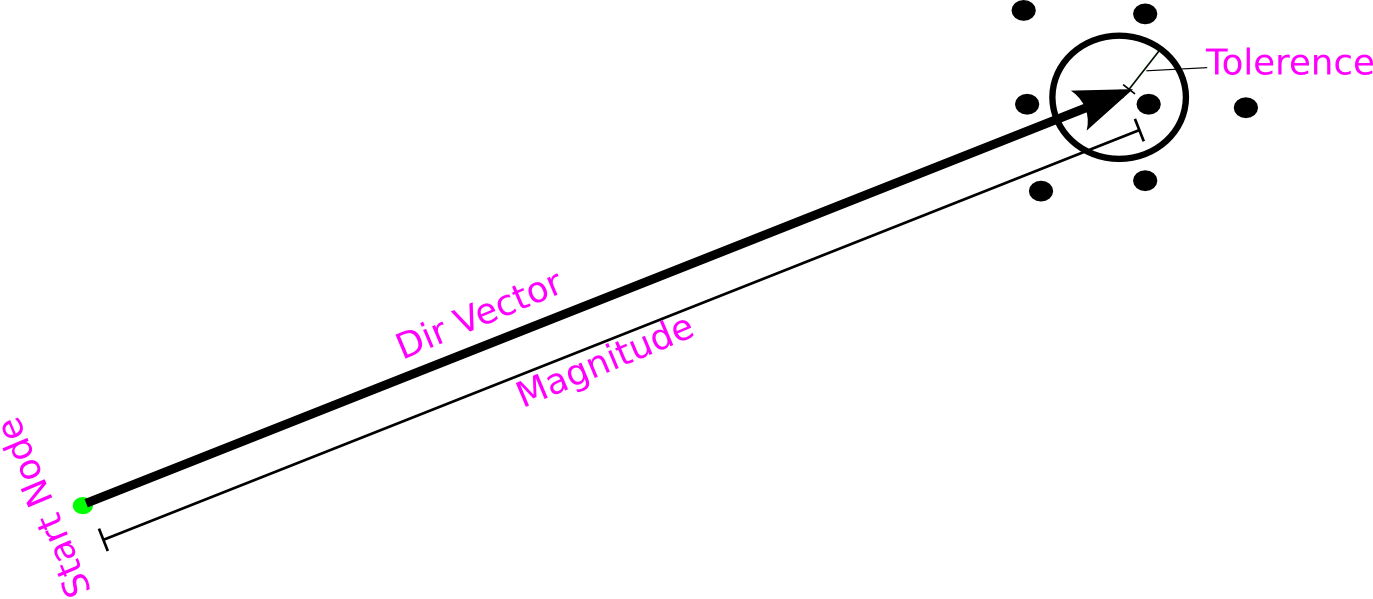
\includegraphics[scale = 2.2]
        {Images/ConnectCommand.png}
        \caption{\label{Connect-command} Pictorial representation of working of connect command}
      \end{figure}

    \item This command updates creates \textbf{additional nodes and 2-noded elements} and \textbf{also assigns a physical group name \textcolor{violet}{"\$New\_Physical\_Group\_Name\$"}}. gmESSI automatically adds the next id available to the new physical group. The user can then manupulate this newly created physical group with any other gmESSI commands.

  \end{itemize}

The working of this command would be more clear through an example.
\textbf{\textit{\href{http://beta.sumeetsinha.in/gmESSI/Examples/Example2}{
Example2 }}} and
\textbf{\textit{\href{http://beta.sumeetsinha.in/gmESSI/Examples/Example3}{
Example3 }}} describes two situtaion one where \textbf{new nodes are to be
created} and the other \textbf{where allready present nodes needs to be found}
respectively. In both the cases \textbf{2-noded line elements} are always
created.\\

\textbf{\href{http://beta.sumeetsinha.in/gmESSI/Examples/Example2}{ Example2}}
creates a contact elements between two prallell surfaces, described by physical
group 1 and 2 respectively. Let us look at the
\href{http://beta.sumeetsinha.in/gmESSI/Examples/Example2/Example2.geo}{
Example2.geo } file.

\begin{lstlisting}[language=C]
$ cat Example2.geo

  Point(1)= {0,0,0}; Point(2) ={0,0,1};
  Extrude{1,0,0} {Point{1,2};Layers{10};Recombine;}
  Extrude{0,1,0} {Line{1,2};Layers{10};Recombine;}
  Physical Surface ("$Surface1$ ") ={6};
  // Generating 1 layers of elements between Physical group 1 and 2
  Physical Surface ("$Surface2$ [Connect{Physical_Group#1, Physical_Group#2, Physical_Group#2,0\0\1,1 , 1, create, 0.005, My_New_Physical_Group}]") ={10};
  // Generating 5 layers of elements between Physical group 1 and 2
  // Physical Surface ("$Surface2$ [Connect{Physical_Group#1, Physical_Group#2, Physical_Group#2,0\0\1,0.2 , 5, create, 0.005, My_New_Physical_Group}]") ={10};
\end{lstlisting}

  \noindent Running \href{http://beta.sumeetsinha.in/gmESSI/Examples/Example2}{
  Example2.msh } with gmESSI, produces additional nodes and elements as shown
  in FigureFigure~\ref{Example-2} . \textbf{Please note "create" in the gmESSI command (b) and (c)
  refers to create new nodes}. 

\begin{figure}[h]
  \centering
  \begin{subfigure}[b]{0.3\textwidth}
    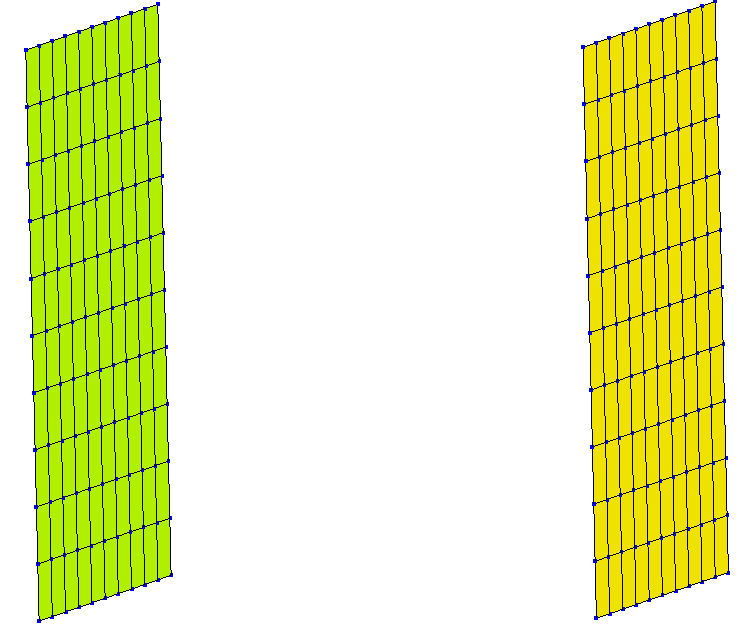
\includegraphics[width=\textwidth,angle=90]{Images/Example2-OriginalMesh.png}
    \caption{Initial mesh file Example2.msh genearet by gmsh. The dir vector is in Z axis {0,0,1} }
  \end{subfigure}\hfill
  \begin{subfigure}[b]{0.3\textwidth}
    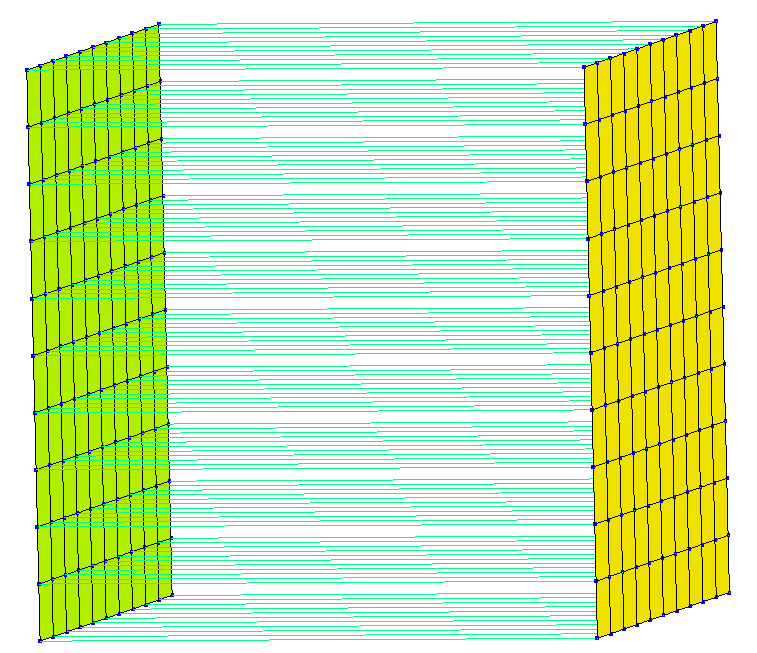
\includegraphics[width=\textwidth,angle=90]{Images/Example2-1Layer.png}
    \caption{1 layer of contact elements \textcolor{violet}{[Connect\{Physical\_Group\#1, Physical\_Group\#2, Physical\_Group\#2, {0\textbackslash0\textbackslash1}, 1, 1, create, 0.005, My_New_Physical_Group\}]}}
  \end{subfigure}\hfill
    \begin{subfigure}[b]{0.3\textwidth}
    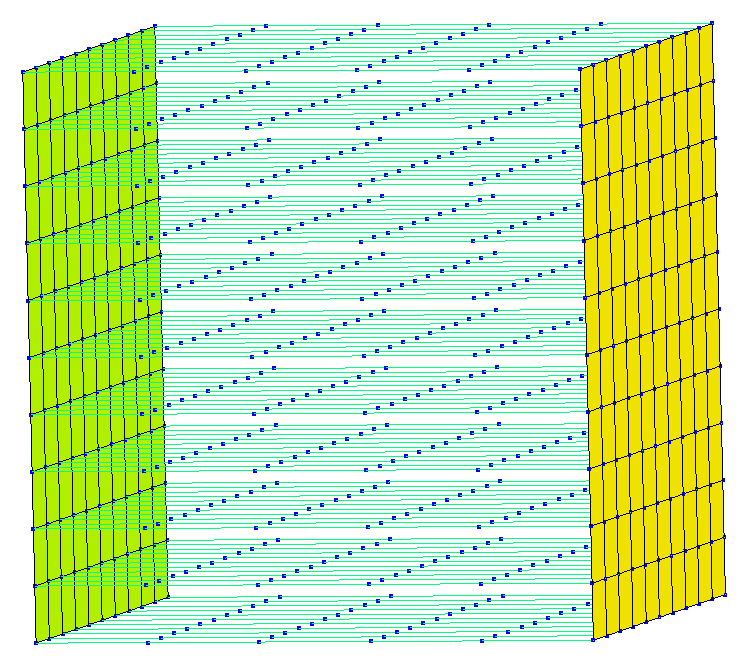
\includegraphics[width=\textwidth,angle=90]{Images/Example2-5Layers.png}
    \caption{5 Layers of contact elements \textcolor{violet}{[Connect\{ Physical\_Group\#1, Physical\_Group\#2, Physical\_Group\#2, {0\textbackslash0\textbackslash1} ,0.2, 5, create, 0.005, My_New_Physical_Group\}]}}
  \end{subfigure}
  \caption{\label{Example-2} Example 2 Contact Problem. (b) and (c) shows the nodes and elements generated by gmESSI Translator. }
\end{figure}

  
The termminal displays the information about
number of elements and nodes created and also displays the information about
the new physical group information i.e id and name. The new physical group
creation can be seen in the \href
{http://beta.sumeetsinha.in/gmESSI/Examples/Example2/Example2_ESSI_Simulation
/Example2.msh}{ Example2.msh } file saves in Example2\_ESSI\_Simulation
folder. The terminal message and mesh file is shown below. It also displays
error message if more than one node is found in the tolerence provided.

\begin{lstlisting}[language=C]
$ gmessi Example2.msh

  Connect{Physical_Group#1,Physical_Group#2, Physical_Group#3, {0\0\1}, 1, 1, create, 0.005, My_New_Physical_Group}  Found!!  Sucessfully Converted
  <@\textcolor{blue}{New Physical Group "My_New_Physical_Group" having id 3 consisting of 242 Nodes and 121 2-noded elements created }@>

\end{lstlisting}

\begin{lstlisting}[language=C]
$ cat Example2_ESSI_Simulation\Example2.msh
  ............
  $PhysicalNames
  3
  2 1 "$Surface1$ "
  2 2 "$Surface2$ [Connect{Physical_Group#1, Physical_Group#2, Physical_Group#2, 0/0/1, 1, 1, create, 0.005, My_New_Physical_Group}]"
  1 3 "$My_New_Physical_Group$"
  $EndPhysicalNames
  ...........
\end{lstlisting}

\noindent \textbf{\href{http://beta.sumeetsinha.in/gmESSI/Examples/Example3}{ Example3 }}
describes a solid cube where a physical group of all the 2-noded elements
joining the nodes from physical surface 1 to 2 needs to be initialized. This
physical group can then be manupulated by the user for any other gmESSI command
like defining beam elements ... etc. Here the task is to find textbf{(algo
'find')} the allready present nodes and textbf{create 2-noded elements}. Let us
look at the
\href{http://beta.sumeetsinha.in/gmESSI/Examples/Example3/Example3.geo}{
Example3.geo } file.

\begin{lstlisting}[language=C]
$ cat Example3.geo

  Point(1)= {0,0,0}; 
  Extrude{1,0,0} {Point{1};Layers{10};Recombine;}
  Extrude{0,1,0} {Line{1};Layers{10};Recombine;}
  Extrude{0,0,1} {Surface{5};Layers{10};Recombine;}
  Physical Surface ("$Surface1$ ") ={5};
  // Generating 1 layers of elements between Physical group 1 and 2
  Physical Surface ("$Surface2$ [Connect{Physical_Group#1, Physical_Group#2, Physical_Group#3, 0\0\1, 1, 1, find, 0.005}]") ={27};
  // Generating 5 layers of elements between Physical group 1 and 2
  // Physical Surface ("$Surface2$ [Connect{Physical_Group#1, Physical_Group#2, Physical_Group#3, 0\0\1, 0.2, 5, find, 0.005}]") ={27};
  Physical Volume  ("$Volume$") ={1};

\end{lstlisting}

\begin{figure}[h]
  \centering
  \begin{subfigure}[b]{0.3\textwidth}
    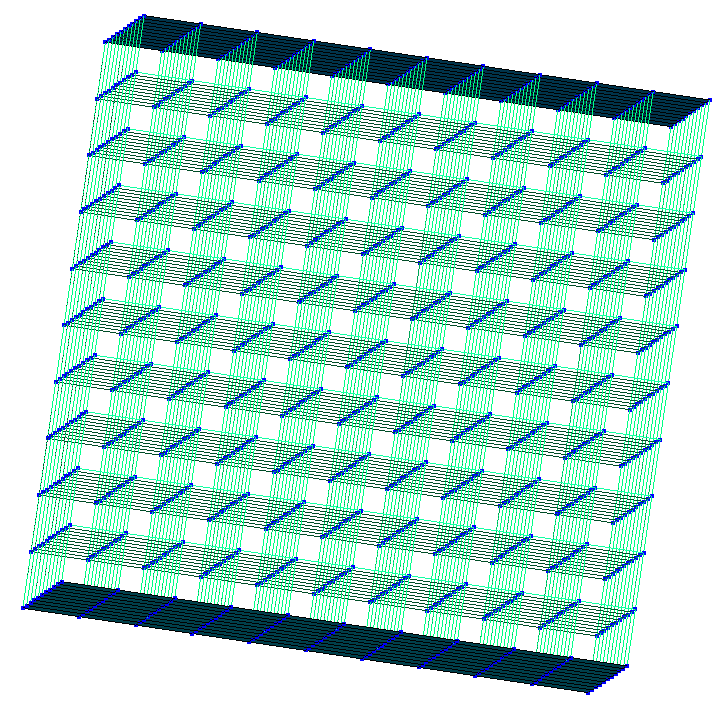
\includegraphics[width=\textwidth]{Images/Example3-OriginalMesh.png}
    \caption{Initial mesh file Example3.msh genearet by gmsh. The dir vector is in Z axis {0,0,1} }
  \end{subfigure}\hfill
  \begin{subfigure}[b]{0.3\textwidth}
    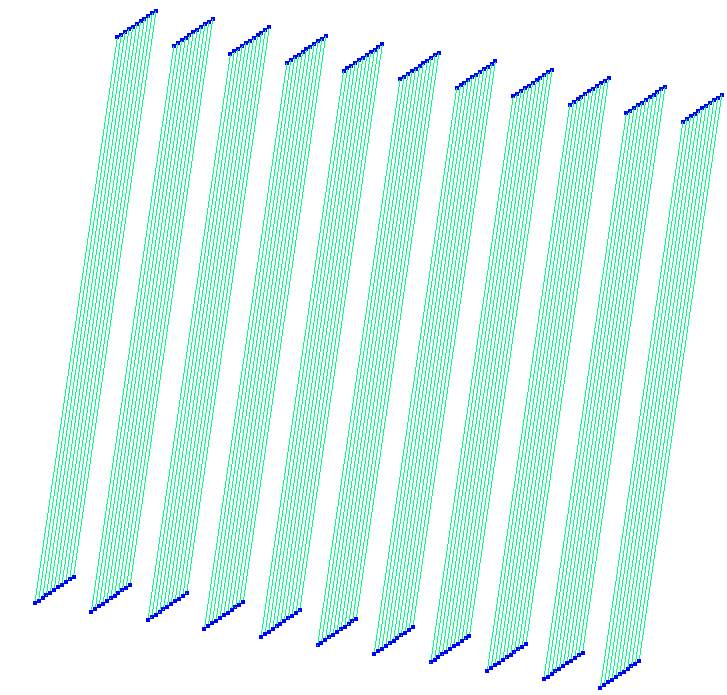
\includegraphics[width=\textwidth]{Images/Example3-1Layer.png}
    \caption{New physical group 4 of 1 Layer of elements \textcolor{violet}{[Connect\{Physical\_Group\#1, Physical\_Group\#2, Physical\_Group\#3, 0\textbackslash0\textbackslash1, 1, 1, 0, find, 005, My_New_Physical_Group\}]}}
  \end{subfigure}\hfill
    \begin{subfigure}[b]{0.3\textwidth}
    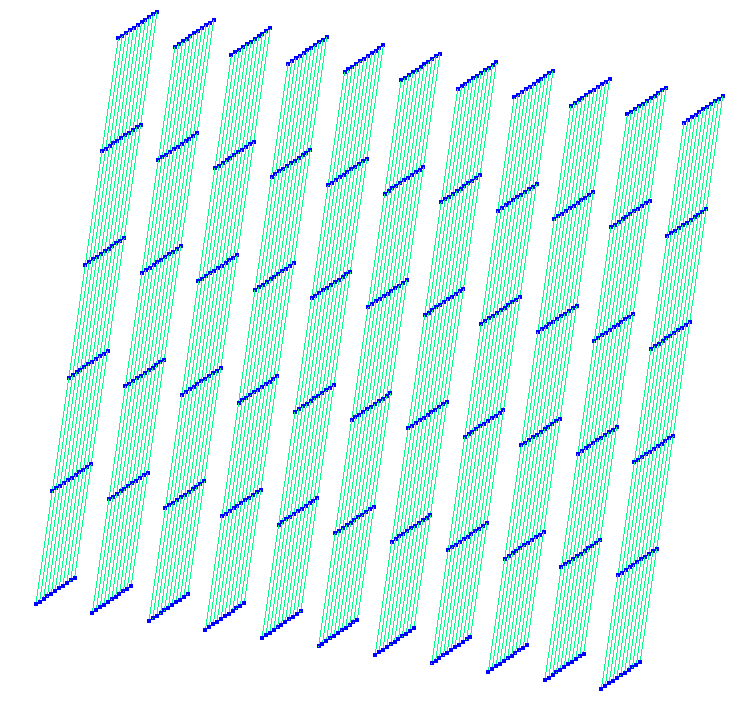
\includegraphics[width=\textwidth]{Images/Example3-5layers.png}
    \caption{New physical group 4 of 5 Layers of elements \textcolor{violet}{[Connect\{ Physical\_Group\#1, Physical\_Group\#2, Physical\_Group\#3, 0\textbackslash0\textbackslash1 ,0.2, 5, find, 0.005, My_New_Physical_Group\}]}}
  \end{subfigure}
  \caption{\label{Example-3-Connect-Command}Example 3 finding nodes problem. (b)
  and (c) shows the nodes and elements generated by gmESSI Translator. }
\end{figure}

Similarly the \href{http://beta.sumeetsinha.in/gmESSI/Examples/Example3/Exampl
e3_ESSI_Simulation/Example3.msh}{ Example3.msh } contains the new physical
group and terminal shows the new physical group of 2-noded elements created.
Figure~\ref{Example-3-Connect-Command} shows the new nodes found and creation of
2-noded elements.

\begin{lstlisting}[language=C]
$ gmESSI Example3.msh

  Connect{Physical_Group#1, Physical_Group#2, Physical_Group#3, {0\0\1}, 1, 1, find, 0.005, My_New_Physical_Group}  Found!!
  <@\textcolor{blue}{New Physical Group "My_New_Physical_Group" having id 4 consisting of 242 Nodes and 121 2-noded elements created }@>

\end{lstlisting}

\begin{lstlisting}[language=C]
$ cat Example3_ESSI_Simulation\Example3.msh
  ............
  $PhysicalNames
  3
  2 1 "$Surface1$ "
  2 2 "$Surface2$ [Connect{Physical_Group#1, Physical_Group#2, Physical_Group#3,{0\0\1}, 1, 1, find, 0.005, My_New_Physical_Group}]"
  3 3 "$Volume$"
  1 4 "$My_New_Physical_Group$"
  $EndPhysicalNames
  ...........
\end{lstlisting}

\noindent \textbf{Please note} that since the algo is to find the nodes so no new nodes
  are created but only elements are created. The same message can be ssen on
  the terminal.

%%%%%%%%%%%%%%%%%%%%%%%%%%%%%%%%%%%%%%%%%%%%%%%%%%%%%%%%%%%%%%%%%%%%%%%%%%%%%%%
\subsubsection{Material Variational command}

Material Variational command is a special command to \textit{define
different element's material properties throughtout the physical/entity group}
based on a function for each material parameter varying with the elements
coordinate in (x,y,z). The corresponding new materials are written in the main
\textbf{XYZ_analysis.fei} and the elements definition are written in
\textbf{XYZ_geometry.fei}. This command is extremely useful if you want to
assign different material properties to different layers let say as soil. This
commands work on physical/entity group of elements. In this command each
material property is like a \textbf{mathematical function of f(x,y,z)}. The
function gets evaluated in octave, so one can write anything that octave can
understand.

All the material properties are as a function and has two optional parameters
\textbf{precision} and \textbf{unit} separate by separator '\textbackslash' . A
typical syntax of this type of command is explained below. An working example
of this command is shown later \\


\centerline{\textcolor{violet}{[Vary\_Material\{Elemental\_Comm\{a,b\},
Par1_fun\textbackslash Prec \textbackslash Unit, Par1_fun\textbackslash Prec
\textbackslash Unit,.......\} }]}


\noindent \\ \textbf{Vary\_Material  ::} It refers to the name of the command. The
name of the   command   is   \textit{Vary_materialname}.   For  example:  to 
vary  a \textit{Linear\_elastic\_isotropic\_3d}      the      command     name  
is \textcolor{violet} { Vary\_Linear\_elastic\_isotropic\_3d } \\ 

\noindent \textbf{Elemental\_Command\{a,b\} ::} It refers to the name of the
elemental command defined in section 5.3. The elemental command refer to the
type of element to define and apply material for the given physical group. The
elemental command is the same as in section 5.3 but has no "mataerial_no" and
the arguments are seprated "," as earlier. For example:- an elemental command

\textcolor{violet}{Add\_Beam\_Displacement\_Based\{ material\_no, section\_no,
mass\_density, integration\_rule, xz\_plane\_vector\_x, xz\_plane\_vector\_y,
xz\_plane\_vector\_z, joint\_1\_offset\_1, joint\_1\_offset\_2,
joint\_1\_offset\_3, joint\_2\_offset\_1, joint\_2\_offset\_2,
joint\_2\_offset\_3\}} \\ would change to

\textcolor{violet}{Add\_Beam\_Displacement_Based(section_no; mass\_density;
integration\_rule; xz\_plane\_vector\_x; xz\_plane\_vector\_y; xz\_plane\_vector\_z;
joint\_1\_offset\_1; joint\_1\_offset\_2; joint\_1\_offset\_3; joint\_2\_offset\_1;
joint\_2\_offset\_2; joint\_2\_offset\_3)}  

\noindent \textbf{Note that} material\_no parameter
has been removed from the command and then incorporated in material\_variational command. \\

\noindent \textbf{Par1_function ::} All the properties/parameters of the
material command is like a function in terms of variable $x,y,z$ like
$14100*x+y$. If any parameter is a string it should be written withing double
quotes "" like \textit{algorithm type} in \textbf{ESSI} is a string and thus can
be written as \textit{"implicit"}. \\

\noindent \textbf{Precision ::} Precision is applied on the output of \textit
{parameter\_function}. It is optional but if written, it should be separated
from parameter\_function by \textbackslash. A precision value can be any integer
i.e \textbf{+ve}, \textbf{-ve} or \textbf{0}.

  \begin{itemize} 

    \item \textbf{+n  - } It refers to rounding of the  parameter\_function
    output upto \textbf{n} significant digits in decimals. Example:- A
    precision of 3 and 2 applied to 163.23647 will produce 163.236 and 163.24
    respectively.

    \item \textbf{0  - } It refers to rounding of the  parameter\_function
    output to an integer. Example:- A precision of 0 applied to 163.23647 will
    produce 163.

    \item \textbf{-n  - } It refers to rounding of the  parameter\_function
    output upto {${10^n}th$} place in number system. Example:- A precision of
    -3 and -2 applied to 163.23647 will produce 200 and 170 respectively.

  \end{itemize}

\noindent \textbf{Unit ::} It refers to unit of the material\_parameter. It is
optional but if written, it should be separated from Precision by
\textbackslash.\\

\noindent\textbf{Note:-} Every Material Variational command has the option of
adding \textcolor{violet}{Physical\_Group/Entity\_Group\#} argument in the
front. \\

To illustrate an example of material variational command, \href
{http://beta.sumeetsinha.in/gmESSI/Examples/Example3/Example3\_ESSI\_Simulation/Example3\_geometry.fei} {
Example3\_geometry.fei}
is again used. Then Material variational command is applied on the
\textbf{"Volume"} physical group to define layers of 8 noded bricks with varying
material Linear\_elastic\_isotropic\_3d\ property. Let say we increase the
\textit{Elastic modulus and density } of the 8noded-bricks down the depth in -z
direction.

\begin{lstlisting}[language=C]
$ cat Example3.geo

  Point(1)= {0,0,0}; 
  Extrude{1,0,0} {Point{1};Layers{10};Recombine;}
  Extrude{0,1,0} {Line{1};Layers{10};Recombine;}
  Extrude{0,0,1} {Surface{5};Layers{10};Recombine;}
  Physical Surface ("$Surface1$ ") ={5};
  // Generating 1 layers of elements between Physical group 1 and 2
  Physical Surface ("$Surface2$ [Connect{Physical_Group#1,Physical_Group#2,Physical_Group#3,0\0\1,1,1,0,0.005, My_New_Physical_Group}]") ={27};
  // Generating 5 layers of elements between Physical group 1 and 2
  // Physical Surface ("$Surface2$ [Connect{Physical_Group#1,Physical_Group#2,Physical_Group#3,0\0\1,0.2,5,1,0.005, My_New_Physical_Group}]") ={27};
  Physical Volume  ("$Volume$ [Vary_Linear_elastic_isotropic_3d{Add_8NodeBrick{},
    1600-100*(1-z)\0\kg/m^3,2*10^9-(1-z)*10^8\0\Pa,0.35}]") ={1};

\end{lstlisting}

When \href
{http://beta.sumeetsinha.in/gmESSI/Examples/Example3/Example3.msh} {
Example3.msh} is translated using gmESSI, it creates 8-noded bricks and assign
different matrials layer-wise. The content  of Example3\_analysis.fei file contains all new declared materials as shown below

\begin{lstlisting}[language=C]
$ cat Example3_analysis.fei

  add material #1 type linear_elastic_isotropic_3d mass_density=1505.000000*kg/m^3 elastic_modulus=1904999936.000000*Pa poisson_ratio=0.35;
  add material #2 type linear_elastic_isotropic_3d mass_density=1515.000000*kg/m^3 elastic_modulus=1915000064.000000*Pa poisson_ratio=0.35;
  add material #3 type linear_elastic_isotropic_3d mass_density=1525.000000*kg/m^3 elastic_modulus=1924999936.000000*Pa poisson_ratio=0.35;
  add material #4 type linear_elastic_isotropic_3d mass_density=1535.000000*kg/m^3 elastic_modulus=1935000064.000000*Pa poisson_ratio=0.35;
  add material #5 type linear_elastic_isotropic_3d mass_density=1545.000000*kg/m^3 elastic_modulus=1944999936.000000*Pa poisson_ratio=0.35;
  add material #6 type linear_elastic_isotropic_3d mass_density=1555.000000*kg/m^3 elastic_modulus=1955000064.000000*Pa poisson_ratio=0.35;
  add material #7 type linear_elastic_isotropic_3d mass_density=1565.000000*kg/m^3 elastic_modulus=1964999936.000000*Pa poisson_ratio=0.35;
  add material #8 type linear_elastic_isotropic_3d mass_density=1575.000000*kg/m^3 elastic_modulus=1975000064.000000*Pa poisson_ratio=0.35;
  add material #9 type linear_elastic_isotropic_3d mass_density=1585.000000*kg/m^3 elastic_modulus=1984999936.000000*Pa poisson_ratio=0.35;
  add material #10 type linear_elastic_isotropic_3d mass_density=1595.000000*kg/m^3 elastic_modulus=1995000064.000000*Pa poisson_ratio=0.35;

\end{lstlisting}

\begin{lstlisting}[language=C]
$ cat Example3_geometry.fei
  .....................
  add element #201 type 8NodeBrick with nodes (1,9,117,27,81,198,603,441) use material #1;
  add element #202 type 8NodeBrick with nodes (81,198,603,441,82,199,604,442) use material #2;
  add element #203 type 8NodeBrick with nodes (82,199,604,442,83,200,605,443) use material #3;
  add element #204 type 8NodeBrick with nodes (83,200,605,443,84,201,606,444) use material #4;
  add element #205 type 8NodeBrick with nodes (84,201,606,444,85,202,607,445) use material #5;
  add element #206 type 8NodeBrick with nodes (85,202,607,445,86,203,608,446) use material #6;
  add element #207 type 8NodeBrick with nodes (86,203,608,446,87,204,609,447) use material #7;
  add element #208 type 8NodeBrick with nodes (87,204,609,447,88,205,610,448) use material #8;
  add element #209 type 8NodeBrick with nodes (88,205,610,448,89,206,611,449) use material #9;
  add element #210 type 8NodeBrick with nodes (89,206,611,449,5,45,522,80) use material #10;
  add element #211 type 8NodeBrick with nodes (27,117,118,28,441,603,612,450) use material #1;
  add element #212 type 8NodeBrick with nodes (441,603,612,450,442,604,613,451) use material #2;
  add element #213 type 8NodeBrick with nodes (442,604,613,451,443,605,614,452) use material #3;
  add element #214 type 8NodeBrick with nodes (443,605,614,452,444,606,615,453) use material #4;
  add element #215 type 8NodeBrick with nodes (444,606,615,453,445,607,616,454) use material #5;
  .................
\end{lstlisting}

In \href
{http://beta.sumeetsinha.in/gmESSI/Examples/Example3/Example3_ESSI_Simulation/Example3_analysis.fei} {
Example3_analysis.fei} file, all the materials has been created for
each layer and it can be seen that \textit{mass_density} and
\textit{elastic_modulus} increases down the dept while poisson's ratio is
constant. Similarly, \href
{http://beta.sumeetsinha.in/gmESSI/Examples/Example3/Example3_ESSI_Simulation/Example3_geometry.fei} {
Example3_geometry.fei} shows how 8-nodeBricks are
defined with different materials layer-wise. Different commands available in
this category are listed below

  \begin{itemize}

    \item \textcolor{violet}{gmESSI :: [Vary\_Linear\_elastic\_isotropic\_3d\{Elemental\_Command\{without\_material\_no\_argument\}, mass\_density, elastic\_modulus, poisson\_ratio\} ]}\\
    \textbf{ESSI :: add material \#\{\} type linear\_elastic\_isotropic\_3d mass\_density=\{\} elastic\_modulus=\{\} poisson\_ratio=\{\} } \\
    Description ::  \textit{ add material \# $<.>$ type linear\_elastic\_isotropic\_3d mass\_density = $<M/L^3>$ elastic\_modulus = $<F/L^2>$ poisson\_ratio = $<.>$}

    \item \textcolor{violet}{gmESSI :: [Vary\_Linear\_elastic\_crossanisotropic\{Elemental\_Command\{without\_material\_no\_argument\}, mass\_density, elastic\_modulus\_horizontal, elastic\_modulus\_vertical, poisson\_ratio\_h\_v, poisson\_ratio\_h\_h, shear\_modulus\_h\_v\} ]}\\
    \textbf{ESSI :: add material \#\{\} type linear\_elastic\_crossanisotropic mass\_density=\{\} elastic\_modulus\_horizontal=\{\} elastic\_modulus\_vertical=\{\} poisson\_ratio\_h\_v=\{\} poisson\_ratio\_h\_h=\{\} shear\_modulus\_h\_v=\{\}}\\
    Description ::  \textit{ add material \# $<.>$ type linear\_elastic\_crossanisotropic mass\_density = $<mass\_density>$ elastic\_modulus\_horizontal = $<F/L^2>$ elastic\_modulus\_vertical = $<F/L^2>$ poisson\_ratio\_h\_v = $<.>$ poisson\_ratio\_h\_h = $<.>$ shear\_modulus\_h\_v = $<F/L^2>$}

    \item \textcolor{violet}{gmESSI :: [Vary\_Vonmises\_perfectly\_plastic\{Elemental\_Command\{without\_material\_no\_argument\}, mass\_density, elastic\_modulus, poisson\_ratio, von\_mises\_radius, initial\_confining\_stress, initial\_confining\_stress, algorithm, number\_of\_subincrements, maximum\_number\_of\_iterations, tolerance\_1, tolerance\_2\}]}\\
    \textbf{ESSI :: add material \#\{\} type vonmises\_perfectly\_plastic mass\_density=\{\} elastic\_modulus=\{\} poisson\_ratio=\{\}  von\_mises\_radius=\{\} initial\_confining\_stress=\{\} algorithm=\{\} number\_of\_subincrements=\{\} maximum\_number\_of\_iterations=\{\} tolerance\_1=\{\} tolerance\_2=\{\} } \\
    Description ::  \textit{ add material \# $<.>$ type vonmises\_perfectly\_plastic mass\_density = $<M/L^3>$ elastic\_modulus = $<F/L^2>$ poisson\_ratio = $<.>$ von\_mises\_radius = $<F/L^2>$ initial\_confining\_stress = $<F/L^2>$ algorithm = $<explicit|implicit>$ number\_of\_subincrements = $<.>$ maximum\_number\_of\_iterations = $<.>$ tolerance\_1 = $<.>$ tolerance\_2 = $<.>$} 

    \item \textcolor{violet}{gmESSI :: [Vary\_Vonmises\_perfectly\_plastic\_accelerated\{Elemental\_Command\{without\_material\_no\_argument\}, mass\_density, elastic\_modulus, poisson\_ratio, von\_mises\_radius, initial\_confining\_stress, maximum\_number\_of\_iterations, tolerance\_1, tolerance\_2\}]}\\
    \textbf{ESSI :: add material \#\{\} type vonmises\_perfectly\_plastic\_accelerated mass\_density=\{\} elastic\_modulus=\{\} poisson\_ratio=\{\} von\_mises\_radius=\{\} initial\_confining\_stress=\{\}  maximum\_number\_of\_iterations=\{\}  tolerance\_1=\{\}  tolerance\_2=\{\}}\\
    Description ::  \textit{ add material \# $<.>$ type vonmises\_perfectly\_plastic\_accelerated mass\_density = $<M/L^3>$ elastic\_modulus = $<F/L^2>$ poisson\_ratio = $<.>$ von\_mises\_radius = $<F/L^2>$ initial\_confining\_stress = $<F/L^2>$  maximum\_number\_of\_iterations = $<.>$ tolerance\_1 = $<.>$ tolerance\_2 = $<.>$} 

    \item \textcolor{violet}{gmESSI :: [Vary\_Vonmises\_isotropic\_hardening\{Elemental\_Command\{without\_material\_no\_argument\}, mass\_density, elastic\_modulus, poisson\_ratio, von\_mises\_radius, isotropic\_hardening\_rate, initial\_confining\_stress, algorithm, number\_of\_subincrements, maximum\_number\_of\_iterations, tolerance\_1, tolerance\_2\}]}\\
    \textbf{ESSI :: add material \#\{\} type vonmises\_isotropic\_hardening mass\_density=\{\} elastic\_modulus=\{\}  poisson\_ratio=\{\}  von\_mises\_radius=\{\}  isotropic\_hardening\_rate=\{\}  initial\_confining\_stress=\{\} algorithm=\{\}  number\_of\_subincrements=\{\}  maximum\_number\_of\_iterations=\{\}  tolerance\_1=\{\}  tolerance\_2=\{\}}\\
    Description ::  \textit{ add material \# $<.>$ type vonmises\_isotropic\_hardening mass\_density = $<M/L^3>$ elastic\_modulus = $<F/L^2>$ poisson\_ratio = $<.>$ von\_mises\_radius = $<F/L^2>$ isotropic\_hardening\_rate = $<F/L^2>$ initial\_confining\_stress = $<F/L^2>$ algorithm = $<explicit|implicit>$ number\_of\_subincrements = $<.>$ maximum\_number\_of\_iterations = $<.>$ tolerance\_1 = $<.>$ tolerance\_2 = $<.>$} 

    \item \textcolor{violet}{gmESSI :: [Vary\_Vonmises\_isotropic\_hardening\_accelerated\{Elemental\_Command\{without\_material\_no\_argument\}, mass\_density, elastic\_modulus, poisson\_ratio, von\_mises\_radius, isotropic\_hardening\_rate, initial\_confining\_stress, maximum\_number\_of\_iterations, tolerance\_1, tolerance\_2\} ]}\\
    \textbf{ESSI :: add material \#\{\} type vonmises\_isotropic\_hardening\_accelerated mass\_density=\{\} elastic\_modulus=\{\} poisson\_ratio=\{\} von\_mises\_radius=\{\} isotropic\_hardening\_rate=\{\} initial\_confining\_stress=\{\} maximum\_number\_of\_iterations=\{\} tolerance\_1=\{\} tolerance\_2=\{\} } \\
    Description ::  \textit{ add material \# $<.>$ type vonmises\_isotropic\_hardening\_accelerated mass\_density = $<M/L^3>$ elastic\_modulus = $<F/L^2>$ poisson\_ratio = $<.>$ von\_mises\_radius = $<F/L^2>$ isotropic\_hardening\_rate = $<F/L^2>$ initial\_confining\_stress = $<F/L^2>$  maximum\_number\_of\_iterations = $<.>$ tolerance\_1 = $<.>$ tolerance\_2 = $<.>$} 

    \item \textcolor{violet}{gmESSI :: [Vary\_Vonmises\_kinematic\_hardening\{Elemental\_Command\{without\_material\_no\_argument\}, mass\_density, elastic\_modulus, poisson\_ratio, von\_mises\_radius, armstrong\_frederick\_ha, armstrong\_frederick\_cr, initial\_confining\_stress, algorithm, number\_of\_subincrements, maximum\_number\_of\_iterations, tolerance\_1, tolerance\_2\}]}\\
    \textbf{ESSI :: add material \#\{\} type vonmises\_kinematic\_hardening mass\_density=\{\} elastic\_modulus=\{\} poisson\_ratio=\{\} von\_mises\_radius=\{\} armstrong\_frederick\_ha=\{\} armstrong\_frederick\_cr=\{\} initial\_confining\_stress=\{\} algorithm=\{\} number\_of\_subincrements=\{\} maximum\_number\_of\_iterations=\{\} tolerance\_1=\{\} tolerance\_2=\{\}}\\
    Description ::  \textit{ add material \# $<.>$ type vonmises\_kinematic\_hardening mass\_density = $<M/L^3>$ elastic\_modulus = $<F/L^2>$ poisson\_ratio = $<.>$ von\_mises\_radius = $<F/L^2>$ armstrong\_frederick\_ha = $<F/L^2>$ armstrong\_frederick\_cr = $<F/L^2>$ initial\_confining\_stress = $<F/L^2>$ algorithm = $<explicit|implicit>$ number\_of\_subincrements = $<.>$ maximum\_number\_of\_iterations = $<.>$ tolerance\_1 = $<.>$ tolerance\_2 = $<.>$} 

    \item \textcolor{violet}{gmESSI :: [Vary\_Vonmises\_linear\_kinematic\_hardening\{Elemental\_Command\{without\_material\_no\_argument\}, mass\_density, elastic\_modulus, poisson\_ratio, von\_mises\_radius, kinematic\_hardening\_rate, initial\_confining\_stress, algorithm, number\_of\_subincrements, maximum\_number\_of\_iterations, tolerance\_1, tolerance\_2\}]}\\
    \textbf{ESSI :: add material \#\{\} type vonmises\_linear\_kinematic\_hardening mass\_density=\{\} elastic\_modulus=\{\} poisson\_ratio=\{\} von\_mises\_radius=\{\} kinematic\_hardening\_rate=\{\} initial\_confining\_stress=\{\} algorithm=\{\} number\_of\_subincrements=\{\} maximum\_number\_of\_iterations=\{\} tolerance\_1=\{\} tolerance\_2=\{\}}\\
    Description ::  \textit{ add material \# $<.>$ type vonmises\_linear\_kinematic\_hardening mass\_density = $<M/L^3>$ elastic\_modulus = $<F/L^2>$ poisson\_ratio = $<.>$ von\_mises\_radius = $<F/L^2>$ kinematic\_hardening\_rate = $<.>$ initial\_confining\_stress = $<F/L^2>$ algorithm = $<explicit|implicit>$ number\_of\_subincrements = $<.>$ maximum\_number\_of\_iterations = $<.>$ tolerance\_1 = $<.>$ tolerance\_2 = $<.>$} 

    \item \textcolor{violet}{gmESSI :: [Vary\_Vonmises\_kinematic\_hardening\_accelerated\{Elemental\_Command\{without\_material\_no\_argument\}, mass\_density, elastic\_modulus, poisson\_ratio, von\_mises\_radius, armstrong\_frederick\_ha, armstrong\_frederick\_cr, initial\_confining\_stress, initial\_confining\_strain, maximum\_number\_of\_iterations, tolerance\_1, tolerance\_2\}]}\\
    \textbf{ESSI :: add material \#\{\} type vonmises\_kinematic\_hardening\_accelerated mass\_density=\{\} elastic\_modulus=\{\} poisson\_ratio=\{\} von\_mises\_radius=\{\} armstrong\_frederick\_ha=\{\} armstrong\_frederick\_cr=\{\} initial\_confining\_stress=\{\} initial\_confining\_strain=\{\} maximum\_number\_of\_iterations=\{\} tolerance\_1=\{\} tolerance\_2=\{\}}\\
    Description ::  \textit{ add material \# $<.>$ type vonmises\_kinematic\_hardening\_accelerated mass\_density = $<M/L^3>$ elastic\_modulus = $<F/L^2>$ poisson\_ratio = $<.>$ von\_mises\_radius = $<F/L^2>$ armstrong\_frederick\_ha = $<F/L^2>$ armstrong\_frederick\_cr = $<F/L^2>$ initial\_confining\_stress = $<F/L^2>$ initial\_confining\_strain = $<.>$ maximum\_number\_of\_iterations = $<.>$ tolerance\_1 = $<.>$ tolerance\_2 = $<.>$} 

    \item \textcolor{violet}{gmESSI :: [Vary\_Vonmises\_linear\_kinematic\_hardening\_accelerated\{Elemental\_Command\{without\_material\_no\_argument\}, mass\_density, elastic\_modulus, poisson\_ratio, von\_mises\_radius, kinematic\_hardening\_rate, initial\_confining\_stress, initial\_confining\_strain, maximum\_number\_of\_iterations, tolerance\_1, tolerance\_2\}]}\\
    \textbf{ESSI :: add material \#\{\} type vonmises\_linear\_kinematic\_hardening\_accelerated mass\_density=\{\} elastic\_modulus=\{\} poisson\_ratio=\{\} von\_mises\_radius=\{\} kinematic\_hardening\_rate=\{\} initial\_confining\_stress=\{\} initial\_confining\_strain=\{\} maximum\_number\_of\_iterations=\{\} tolerance\_1=\{\} tolerance\_2=\{\}}\\
    Description ::  \textit{ add material \# $<.>$ type vonmises\_linear\_kinematic\_hardening\_accelerated mass\_density = $<M/L^3>$ elastic\_modulus = $<F/L^2>$ poisson\_ratio = $<.>$ von\_mises\_radius = $<F/L^2>$ kinematic\_hardening\_rate = $<.>$ initial\_confining\_stress = $<F/L^2>$ initial\_confining\_strain = $<.>$ maximum\_number\_of\_iterations = $<.>$ tolerance\_1 = $<.>$ tolerance\_2 = $<.>$} 

    \item \textcolor{violet}{gmESSI :: [Vary\_Vonmises\_perfectly\_plastic\_LT\{Elemental\_Command\{without\_material\_no\_argument\}, mass\_density, elastic\_modulus, poisson\_ratio, von\_mises\_radius,initial\_confining\_stress, algorithm, number\_of\_subincrements, maximum\_number\_of\_iterations, tolerance\_1, tolerance\_2\}]}\\
    \textbf{ESSI :: add material \#\{\} type vonmises\_perfectly\_plastic\_LT mass\_density=\{\} elastic\_modulus=\{\} poisson\_ratio=\{\}  von\_mises\_radius=\{\} initial\_confining\_stress= \{\} algorithm=\{\} number\_of\_subincrements=\{\} maximum\_number\_of\_iterations=\{\} tolerance\_1=\{\} tolerance\_2=\{\}}\\
    Description ::  \textit{ add material \# $<.>$ type vonmises\_perfectly\_plastic\_LT mass\_density = $<M/L^3>$ elastic\_modulus = $<F/L^2>$ poisson\_ratio = $<.>$ von\_mises\_radius = $<F/L^2>$ initial\_confining\_stress = $<F/L^2>$  maximum\_number\_of\_iterations = $<.>$ tolerance\_1 = $<.>$ tolerance\_2 = $<.>$} 

    \item \textcolor{violet}{gmESSI :: [Vary\_VonmisesLT\{Elemental\_Command\{without\_material\_no\_argument\}, mass\_density, elastic\_modulus, poisson\_ratio, vonmises\_radius, kinematic\_hardening\_rate, isotropic\_hardening\_rate\}]}\\
    \textbf{ESSI :: add material \#\{\} type VonMisesLT mass\_density=\{\} elastic\_modulus=\{\}  poisson\_ratio=\{\} von\_mises\_radius=\{\} kinematic\_hardening\_rate=\{\} isotropic\_hardening\_rate=\{\}}\\
    Description ::  \textit{ add material \# $<.>$ type VonMisesLT  mass\_density = $<M/L^3>$ elastic\_modulus = $<F/L^2>$  poisson\_ratio = $<.>$ von\_mises\_radius = $<F/L^2>$ kinematic\_hardening\_rate = $<F/L^2>$ isotropic\_hardening\_rate = $<F/L^2>$} 

    \item \textcolor{violet}{gmESSI :: [Vary\_Druckerprager\_perfectly\_plastic\{Elemental\_Command\{without\_material\_no\_argument\}, mass\_density, elastic\_modulus, poisson\_ratio, druckerprager\_angle, initial\_confining\_stress, algorithm, number\_of\_subincrements, maximum\_number\_of\_iterations, tolerance\_1, tolerance\_2\}]}\\
    \textbf{ESSI :: add material \#\{\} type druckerprager\_perfectly\_plastic mass\_density=\{\} elastic\_modulus=\{\} poisson\_ratio=\{\} druckerprager\_angle=\{\} initial\_confining\_stress=\{\} algorithm=\{\} number\_of\_subincrements=\{\} maximum\_number\_of\_iterations=\{\} tolerance\_1=\{\} tolerance\_2=\{\}}\\
    Description ::  \textit{ add material \# $<.>$ type druckerprager\_perfectly\_plastic  mass\_density = $<M/L^3>$ elastic\_modulus = $<F/L^2>$  poisson\_ratio = $<.>$ druckerprager\_angle = $<F/L^2>$ initial\_confining\_stress = $<F/L^2>$ algorithm = $<explicit|implicit>$  number\_of\_subincrements = $<.>$ maximum\_number\_of\_iterations = $<.>$ tolerance\_1 = $<.>$ tolerance\_2 = $<.>$} 

    \item \textcolor{violet}{gmESSI :: [Vary\_Druckerprager\_perfectly\_plastic\_accelerated\{Elemental\_Command\{without\_material\_no\_argument\}, mass\_density, elastic\_modulus, poisson\_ratio, druckerprager\_angle, initial\_confining\_stress, maximum\_number\_of\_iterations, tolerance\_1, tolerance\_2\}]}\\
    \textbf{ESSI :: add material \#\{\} type druckerprager\_perfectly\_plastic\_accelerated  mass\_density=\{\} elastic\_modulus=\{\}  poisson\_ratio=\{\} druckerprager\_angle=\{\} initial\_confining\_stress=\{\} maximum\_number\_of\_iterations=\{\} tolerance\_1=\{\} tolerance\_2=\{\}}\\
    Description ::  \textit{ add material \# $<.>$ type druckerprager\_perfectly\_plastic\_accelerated  mass\_density = $<M/L^3>$ elastic\_modulus = $<F/L^2>$  poisson\_ratio = $<.>$ druckerprager\_angle = $<F/L^2>$ initial\_confining\_stress = $<F/L^2>$ maximum\_number\_of\_iterations = $<.>$ tolerance\_1 = $<.>$ tolerance\_2 = $<.>$} 

    \item \textcolor{violet}{gmESSI :: [Vary\_Druckerprager\_isotropic\_hardening\{Elemental\_Command\{without\_material\_no\_argument\}, mass\_density, elastic\_modulus, poisson\_ratio, druckerprager\_angle, isotropic\_hardening\_rate, initial\_confining\_stress, algorithm, number\_of\_subincrements, maximum\_number\_of\_iterations, tolerance\_1, tolerance\_2\}]}\\
    \textbf{ESSI :: add material \#\{\} type druckerprager\_isotropic\_hardening mass\_density=\{\} elastic\_modulus=\{\}  poisson\_ratio=\{\} druckerprager\_angle=\{\} isotropic\_hardening\_rate=\{\} initial\_confining\_stress=\{\} algorithm=\{\}  number\_of\_subincrements=\{\} maximum\_number\_of\_iterations=\{\} tolerance\_1=\{\} tolerance\_2=\{\}}\\
    Description ::  \textit{ add material \# $<.>$ type druckerprager\_isotropic\_hardening mass\_density = $<M/L^3>$ elastic\_modulus = $<F/L^2>$  poisson\_ratio = $<.>$ druckerprager\_angle = $<F/L^2>$ isotropic\_hardening\_rate = $<F/L^2>$ initial\_confining\_stress = $<F/L^2>$ algorithm = $<explicit|implicit>$  number\_of\_subincrements = $<.>$ maximum\_number\_of\_iterations = $<.>$ tolerance\_1 = $<.>$ tolerance\_2 = $<.>$} 

    \item \textcolor{violet}{gmESSI :: [Vary\_Druckerprager\_isotropic\_hardening\_accelerated\{Elemental\_Command\{without\_material\_no\_argument\}, mass\_density, elastic\_modulus, poisson\_ratio, druckerprager\_angle, isotropic\_hardening\_rate, initial\_confining\_stress, maximum\_number\_of\_iterations, tolerance\_1, tolerance\_2\} ]}\\
    \textbf{ESSI :: add material \#\{\} type druckerprager\_isotropic\_hardening\_accelerated mass\_density=\{\} elastic\_modulus=\{\}  poisson\_ratio=\{\} druckerprager\_angle=\{\} isotropic\_hardening\_rate=\{\} initial\_confining\_stress=\{\} maximum\_number\_of\_iterations=\{\} tolerance\_1=\{\} tolerance\_2=\{\}}\\
    Description ::  \textit{ add material \# $<.>$ type druckerprager\_isotropic\_hardening\_accelerated mass\_density = $<M/L^3>$ elastic\_modulus = $<F/L^2>$  poisson\_ratio = $<.>$ druckerprager\_angle = $<F/L^2>$ isotropic\_hardening\_rate = $<F/L^2>$ initial\_confining\_stress = $<F/L^2>$ maximum\_number\_of\_iterations = $<.>$ tolerance\_1 = $<.>$ tolerance\_2 = $<.>$} 

    \item \textcolor{violet}{gmESSI :: [Vary\_Druckerprager\_kinematic\_hardening\{Elemental\_Command\{without\_material\_no\_argument\}, mass\_density, elastic\_modulus, poisson\_ratio, druckerprager\_angle, armstrong\_frederick\_ha, armstrong\_frederick\_cr, initial\_confining\_stress, algorithm, number\_of\_subincrements, maximum\_number\_of\_iterations, tolerance\_1, tolerance\_2\}]}\\
    \textbf{ESSI :: add material \#\{\} type druckerprager\_kinematic\_hardening mass\_density=\{\} elastic\_modulus=\{\}  poisson\_ratio=\{\} druckerprager\_angle=\{\} armstrong\_frederick\_ha=\{\} armstrong\_frederick\_cr=\{\} initial\_confining\_stress=\{\} algorithm= \{\}  number\_of\_subincrements=\{\} maximum\_number\_of\_iterations=\{\} tolerance\_1=\{\} tolerance\_2=\{\}}\\
    Description ::  \textit{ add material \# $<.>$ type druckerprager\_kinematic\_hardening  mass\_density = $<M/L^3>$ elastic\_modulus = $<F/L^2>$  poisson\_ratio = $<.>$ druckerprager\_angle = $<F/L^2>$ armstrong\_frederick\_ha = $<F/L^2>$ armstrong\_frederick\_cr = $<F/L^2>$ initial\_confining\_stress = $<F/L^2>$ algorithm = $<explicit|implicit>$  number\_of\_subincrements = $<.>$ maximum\_number\_of\_iterations = $<.>$ tolerance\_1 = $<.>$ tolerance\_2 = $<.>$} 

    \item \textcolor{violet}{gmESSI :: [Vary\_Druckerprager\_kinematic\_hardening\_accelerated\{Elemental\_Command\{without\_material\_no\_argument\}, mass\_density, elastic\_modulus, poisson\_ratio, druckerprager\_angle, armstrong\_frederick\_ha, armstrong\_frederick\_cr, initial\_confining\_stress, maximum\_number\_of\_iterations, tolerance\_1, tolerance\_2\} ]}\\
    \textbf{ESSI :: add material \#\{\} type druckerprager\_kinematic\_hardening\_accelerated mass\_density=\{\} elastic\_modulus=\{\}  poisson\_ratio=\{\} druckerprager\_angle=\{\} armstrong\_frederick\_ha=\{\} armstrong\_frederick\_cr=\{\} initial\_confining\_stress=\{\} maximum\_number\_of\_iterations=\{\} tolerance\_1=\{\} tolerance\_2=\{\}}\\
    Description ::  \textit{ add material \# $<.>$ type druckerprager\_kinematic\_hardening\_accelerated  mass\_density = $<M/L^3>$ elastic\_modulus = $<F/L^2>$  poisson\_ratio = $<.>$ druckerprager\_angle = $<F/L^2>$ armstrong\_frederick\_ha = $<F/L^2>$ armstrong\_frederick\_cr = $<F/L^2>$ initial\_confining\_stress = $<F/L^2>$ maximum\_number\_of\_iterations = $<.>$ tolerance\_1 = $<.>$ tolerance\_2 = $<.>$} 

    \item \textcolor{violet}{gmESSI :: [Vary\_DruckerpragerLT\{Elemental\_Command\{without\_material\_no\_argument\}, mass\_density, elastic\_modulus, poisson\_ratio, druckerprager\_k, kinematic\_hardening\_rate, isotropic\_hardening\_rate\}]}\\
    \textbf{ESSI :: add material \#\{\} type DruckerPragerLT mass\_density=\{\} elastic\_modulus=\{\}  poisson\_ratio=\{\} druckerprager\_k=\{\} kinematic\_hardening\_rate=\{\} isotropic\_hardening\_rate=\{\}}\\
    Description ::  \textit{ add material \# $<.>$ type DruckerPragerLT  mass\_density = $<M/L^3>$ elastic\_modulus = $<F/L^2>$  poisson\_ratio = $<.>$ druckerprager\_k = $<F/L^2>$ kinematic\_hardening\_rate = $<F/L^2>$ isotropic\_hardening\_rate = $<F/L^2>$} 

    \item \textcolor{violet}{gmESSI :: [Vary\_Camclay\{Elemental\_Command\{without\_material\_no\_argument\}, mass\_density, reference\_void\_ratio, critical\_stress\_ratio\_M, lambda, kappa, poisson\_ratio, minimum\_bulk\_modulus, pressure\_reference\_p0, initial\_confining\_stress, algorithm, number\_of\_subincrements, maximum\_number\_of\_iterations, tolerance\_1, tolerance\_2\}]}\\
    \textbf{ESSI :: add material \#\{\} type camclay mass\_density=\{\} reference\_void\_ratio=\{\} critical\_stress\_ratio\_M=\{\} lambda=\{\} kappa=\{\} poisson\_ratio=\{\} minimum\_bulk\_modulus=\{\} pressure\_reference\_p0=\{\} initial\_confining\_stress=\{\} algorithm=\{\} number\_of\_subincrements=\{\} maximum\_number\_of\_iterations=\{\} tolerance\_1=\{\} tolerance\_2=\{\}}\\
    Description ::  \textit{ add material \# $<.>$ type camclay mass\_density = $<M/L^3>$ reference\_void\_ratio = $<.>$ critical\_stress\_ratio\_M = $<.>$ lambda = $<.>$ kappa = $<.>$ poisson\_ratio = $<.>$ minimum\_bulk\_modulus = $<F/L^2>$ pressure\_reference\_p0 = $<F/L^2>$ initial\_confining\_stress = $<F/L^2>$ algorithm = $<explicit|implicit>$  number\_of\_subincrements = $<.>$ maximum\_number\_of\_iterations = $<.>$ tolerance\_1 = $<.>$ tolerance\_2 = $<.>$} 

    \item \textcolor{violet}{gmESSI :: [Vary\_Camclay\_accelerated\{Elemental\_Command\{without\_material\_no\_argument\}, mass\_density, reference\_void\_ratio, critical\_stress\_ratio\_M, lambda, kappa, poisson\_ratio, minimum\_bulk\_modulus, pressure\_reference\_p0, initial\_confining\_stress, maximum\_number\_of\_iterations, tolerance\_1, tolerance\_2\} ]}\\
    \textbf{ESSI :: add material \#\{\} type camclay\_accelerated mass\_density=\{\} reference\_void\_ratio=\{\} critical\_stress\_ratio\_M=\{\} lambda=\{\} kappa=\{\} poisson\_ratio=\{\} minimum\_bulk\_modulus=\{\} pressure\_reference\_p0=\{\} initial\_confining\_stress=\{\}  maximum\_number\_of\_iterations=\{\} tolerance\_1=\{\} tolerance\_2=\{\}}\\
    Description ::  \textit{ add material \# $<.>$ type camclay\_accelerated mass\_density = $<M/L^3>$ reference\_void\_ratio = $<.>$ critical\_stress\_ratio\_M = $<.>$ lambda = $<.>$ kappa = $<.>$ poisson\_ratio = $<.>$ minimum\_bulk\_modulus = $<F/L^2>$ pressure\_reference\_p0 = $<F/L^2>$ initial\_confining\_stress = $<F/L^2>$  maximum\_number\_of\_iterations = $<.>$ tolerance\_1 = $<.>$ tolerance\_2 = $<.>$} 

    \item \textcolor{violet}{gmESSI :: [Vary\_Sanisand2004\{Elemental\_Command\{without\_material\_no\_argument\}, mass\_density, e0, sanisand2004\_G0, poisson\_ratio, sanisand2004\_Pat, sanisand2004\_p\_cut, sanisand2004\_Mc, sanisand2004\_c, sanisand2004\_lambda\_c, sanisand2004\_xi, sanisand2004\_ec\_ref, sanisand2004\_m, sanisand2004\_h0, sanisand2004\_ch, sanisand2004\_nb, sanisand2004\_A0, sanisand2004\_nd, sanisand2004\_z\_max, sanisand2004\_cz, initial\_confining\_stress, algorithm, number\_of\_subincrements, maximum\_number\_of\_iterations, tolerance\_1, tolerance\_2\}]}\\
    \textbf{ESSI :: add material \#\{\} type sanisand2004 mass\_density=\{\} e0=\{\} sanisand2004\_G0=\{\} poisson\_ratio=\{\} sanisand2004\_Pat=\{\}  sanisand2004\_p\_cut=\{\}  sanisand2004\_Mc=\{\}  sanisand2004\_c=\{\} sanisand2004\_lambda\_c=\{\} sanisand2004\_xi=\{\}  sanisand2004\_ec\_ref=\{\}  sanisand2004\_m=\{\}  sanisand2004\_h0=\{\} sanisand2004\_ch=\{\}  sanisand2004\_nb=\{\} sanisand2004\_A0=\{\} sanisand2004\_nd=\{\} sanisand2004\_z\_max=\{\}  sanisand2004\_cz=\{\} initial\_confining\_stress=\{\}  algorithm=\{\}  number\_of\_subincrements=\{\}  maximum\_number\_of\_iterations=\{\}  tolerance\_1=\{\}  tolerance\_2=\{\}}\\
    Description ::  \textit{ add material \# $<.>$ type sanisand2004 mass\_density = $<M/L^3>$ e0 = $<.>$ sanisand2004\_G0 = $<.>$ poisson\_ratio = $<.>$ sanisand2004\_Pat = $<stress>$  sanisand2004\_p\_cut = $<.>$  sanisand2004\_Mc = $<.>$  sanisand2004\_c = $<.>$ sanisand2004\_lambda\_c = $<.>$ sanisand2004\_xi = $<.>$  sanisand2004\_ec\_ref = $<.>$  sanisand2004\_m = $<.>$  sanisand2004\_h0 = $<.>$ sanisand2004\_ch = $<.>$  sanisand2004\_nb = $<.>$ sanisand2004\_A0 = $<.>$ sanisand2004\_nd = $<.>$ sanisand2004\_z\_max = $<.>$  sanisand2004\_cz = $<.>$ initial\_confining\_stress = $<stress>$  algorithm = $<explicit|implicit>$  number\_of\_subincrements = $<.>$  maximum\_number\_of\_iterations = $<.>$  tolerance\_1 = $<.>$  tolerance\_2 = $<.>$} 

    \item \textcolor{violet}{gmESSI :: [Vary\_Sanisand2008\{Elemental\_Command\{without\_material\_no\_argument\}, mass\_density, e0, sanisand2008\_G0, sanisand2008\_K0, sanisand2008\_Pat, sanisand2008\_k\_c, sanisand2008\_alpha\_cc, sanisand2008\_c, sanisand2008\_xi, sanisand2008\_lambda, sanisand2008\_ec\_ref, sanisand2008\_m, sanisand2008\_h0, sanisand2008\_ch, sanisand2008\_nb, sanisand2008\_A0, sanisand2008\_nd, sanisand2008\_p\_r, sanisand2008\_rho\_c, sanisand2008\_theta\_c, sanisand2008\_X, sanisand2008\_z\_max, sanisand2008\_cz, sanisand2008\_p0, sanisand2008\_p\_in, algorithm, number\_of\_subincrements, maximum\_number\_of\_iterations, tolerance\_1, tolerance\_2\}]}\\
    \textbf{ESSI :: add material \#\{\} type sanisand2008 mass\_density=\{\}  e0=\{\}  sanisand2008\_G0=\{\}  sanisand2008\_K0=\{\} sanisand2008\_Pat=\{\} sanisand2008\_k\_c=\{\}  sanisand2008\_alpha\_cc=\{\} sanisand2008\_c=\{\}  sanisand2008\_xi=\{\}  sanisand2008\_lambda=\{\}  sanisand2008\_ec\_ref=\{\}  sanisand2008\_m=\{\}  sanisand2008\_h0=\{\}  sanisand2008\_ch=\{\}  sanisand2008\_nb=\{\}  sanisand2008\_A0=\{\} sanisand2008\_nd=\{\}  sanisand2008\_p\_r=\{\}  sanisand2008\_rho\_c=\{\}  sanisand2008\_theta\_c=\{\}  sanisand2008\_X=\{\}  sanisand2008\_z\_max=\{\}  sanisand2008\_cz=\{\}  sanisand2008\_p0=\{\}  sanisand2008\_p\_in=\{\}  algorithm=\{\}  number\_of\_subincrements=\{\}  maximum\_number\_of\_iterations=\{\}  tolerance\_1=\{\}  tolerance\_2=\{\}}\\
    Description ::  \textit{ add material \# $<.>$ type sanisand2008 mass\_density = $<M/L^3>$  e0 = $<.>$  sanisand2008\_G0 = $<.>$  sanisand2008\_K0 = $<.>$ sanisand2008\_Pat = $<stress>$ sanisand2008\_k\_c = $<.>$  sanisand2008\_alpha\_cc = $<.>$ sanisand2008\_c = $<.>$  sanisand2008\_xi = $<.>$  sanisand2008\_lambda = $<.>$  sanisand2008\_ec\_ref = $<.>$  sanisand2008\_m = $<.>$  sanisand2008\_h0 = $<.>$  sanisand2008\_ch = $<.>$  sanisand2008\_nb = $<.>$  sanisand2008\_A0 = $<.>$ sanisand2008\_nd = $<.>$  sanisand2008\_p\_r = $<.>$  sanisand2008\_rho\_c = $<.>$  sanisand2008\_theta\_c = $<.>$  sanisand2008\_X = $<.>$  sanisand2008\_z\_max = $<.>$  sanisand2008\_cz = $<.>$  sanisand2008\_p0 = $<stress>$  sanisand2008\_p\_in = $<.>$  algorithm = $<explicit|implicit>$  number\_of\_subincrements = $<.>$  maximum\_number\_of\_iterations = $<.>$  tolerance\_1 = $<.>$  tolerance\_2 = $<.>$} 

    \item \textcolor{violet}{gmESSI :: [Vary\_Uniaxial\_elastic\{Elemental\_Command\{without\_material\_no\_argument\}, elastic\_modulus, viscoelastic\_modulus\}]}\\
    \textbf{ESSI :: add material \#\{\} type uniaxial\_elastic elastic\_modulus=\{\} viscoelastic\_modulus=\{\}}\\
    Description ::  \textit{ add material \# $<.>$ type uniaxial\_elastic elastic\_modulus = $<F/L^2>$ viscoelastic\_modulus = $<mass / length / time>$ } 

    \item \textcolor{violet}{gmESSI :: [Vary\_Uniaxial\_concrete02\{Elemental\_Command\{without\_material\_no\_argument\}, comprESSIve\_strength, strain\_at\_comprESSIve\_strength, crushing\_strength, strain\_at\_crushing\_strength, lambda, tensile\_strength, tension\_softening\_stiffness\} ]}\\
    \textbf{ESSI :: add material \#\{\} type uniaxial\_concrete02 comprESSIve\_strength=\{\} strain\_at\_comprESSIve\_strength= \{\} crushing\_strength= \{\}  strain\_at\_crushing\_strength= \{\} lambda=\{\} tensile\_strength=\{\} tension\_softening\_stiffness=\{\}}\\
    Description ::  \textit{ add material \# $<.>$ type uniaxial\_concrete02 comprESSIve\_strength = $<F/L^2>$ strain\_at\_comprESSIve\_strength = $<.>$ crushing\_strength = $<F/L^2>$  strain\_at\_crushing\_strength = $<.>$ lambda = $<.>$ tensile\_strength = $<F/L^2>$ tension\_softening\_stiffness = $<F/L^2>$} 

    \item \textcolor{violet}{gmESSI :: [Vary\_Uniaxial\_steel01\{Elemental\_Command\{without\_material\_no\_argument\},yield\_strength, elastic\_modulus, strain\_hardening\_ratio, a1, a2, a3, a4\}]}\\
    \textbf{ESSI :: add material \#\{\} type uniaxial\_steel01 yield\_strength=\{\} elastic\_modulus=\{\} strain\_hardening\_ratio=\{\} a1=\{\} a2=\{\} a3=\{\} a4=\{\}}\\
    Description ::  \textit{ add material \# $<.>$ type uniaxial\_steel01 yield\_strength = $<F/L^2>$ elastic\_modulus = $<F/L^2>$ strain\_hardening\_ratio = $<.>$  a1 = $<.>$  a2 = $<.>$  a3 = $<>$  a4 = $<.>$ } 

    \item \textcolor{violet}{gmESSI :: [Vary\_Uniaxial\_steel02\{Elemental\_Command\{without\_material\_no\_argument\},yield\_strength, elastic\_modulus, strain\_hardening\_ratio, R0, cR1, cR2, a1, a2, a3, a4\} ]}\\
    \textbf{ESSI :: add material \#\{\} type uniaxial\_steel02 yield\_strength=\{\} elastic\_modulus=\{\} strain\_hardening\_ratio=\{\} R0=\{\} cR1=\{\} cR2=\{\} a1=\{\} a2=\{\} a3=\{\} a4=\{\}}\\
    Description ::  \textit{ add material \# $<.>$ type uniaxial\_steel02 yield\_strength = $<F/L^2>$ elastic\_modulus = $<F/L^2>$ strain\_hardening\_ratio = $<.>$ R0 = $<.>$ cR1 = $<.>$ cR2 = $<.>$  a1 = $<.>$  a2 = $<.>$  a3 = $<>$  a4 = $<.>$ } 

    \item \textcolor{violet}{gmESSI :: [Vary\_New\_PisanoLT\{Elemental\_Command\{without\_material\_no\_argument\},mass\_density, elastic\_modulus, poisson\_ratio, M\_in, kd\_in, xi\_in, h\_in, m\_in, initial\_confining\_stress, n\_in, a\_in, eplcum\_cr\_in\}]}\\
    \textbf{ESSI :: add material \#\{\} type New\_PisanoLT mass\_density=\{\} elastic\_modulus\_1atm=\{\} poisson\_ratio=\{\} M\_in=\{\} kd\_in=\{\} xi\_in=\{\} h\_in=\{\} m\_in=\{\} initial\_confining\_stress=\{\} n\_in =\{\} a\_in =\{\} eplcum\_cr\_in =\{\}}\\
    Description ::  \textit{ add material \# $<.>$ type New\_PisanoLT  mass\_density = $<M/L^2>$ elastic\_modulus\_1atm = $<F/L^2>$ poisson\_ratio = $<.>$ M\_in = $<F/L^2>$ kd\_in = $<.>$ xi\_in = $<.>$ h\_in = $<.>$ m\_in = $<.>$ initial\_confining\_stress = $<F/L^2>$ n\_in = $<.>$ a\_in = $<.>$ eplcum\_cr\_in = $<.>$} 

    \item \textcolor{violet}{gmESSI :: [Vary\_Linear\_elastic\_isotropic\_3d\_LT\{Elemental\_Command\{without\_material\_no\_argument\}, mass\_density, elastic\_modulus, poisson\_ratio\}]}\\
    \textbf{ESSI :: add material \#\{\} type linear\_elastic\_isotropic\_3d\_LT mass\_density=\{\} elastic\_modulus=\{\} poisson\_ratio=\{\} ]}\\
    Description ::  \textit{ add material \# $<.>$ type linear\_elastic\_isotropic\_3d\_LT mass\_density = $<M/L^3>$ elastic\_modulus = $<F/L^2>$ poisson\_ratio = $<.>$} 

  \end{itemize}

%%%%%%%%%%%%%%%%%%%%%%%%%%%%%%%%%%%%%%%%%%%%%%%%%%%%%%%%%%%%%%%%%%%%%%%%%%%%%%%
\subsubsection{Nodal Variational command}
Nodal Variational commands has the similar function as Material variational command 
in which each parameter is like a mathematical function of coordinates i.e $f(x,y,z)$ 
which is evaluated in octave. Whatever is valid for octave is valid for all variational 
commands. Also similiar to Material variational command 
this command has two optional parameters \textbf{precision} and \textbf{unit} separate 
by separator '\textbackslash'. Various commands under this category are 

\noindent \textbf{Note:-} Every Nodal Variational command has the option of adding
\textcolor{violet}{Physical_Group/Entity_Group\#} argument in the front.

\begin{itemize}

  \item \textcolor{violet}{gmESSI :: [Vary\_Node\_Mass\{mx,my,mz\}]}\\
  \textbf{Esssi :: Vary mass to node \#\{\} mx =\{\} my =\{\} mz =\{\}}\\
  Description :: \textit{Vary mass to node \# $<.>$ mx = $<mass>$ my = $<mass>$
  mz = $<mass>$}

  \item \textcolor{violet}{gmESSI :: [Vary\_Node\_Mass\{mx,my,mz,Imx,Imy,Imz\}]} \\ 
  \textbf{Esssi :: Vary mass to node \#\{\} mx =\{\} my =\{\} mz =\{\} Imx =\{\} Imy =\{\} Imz
  =\{\}}\\   Description :: \textit{Vary mass to node \# $<.>$ mx = $<mass>$ my =
  $<mass>$ mz = $<mass>$ Imz = $<mass*length^2>$ Imy = $<mass*length^2>$ Imz =
  $<mass*length^2>$}

  \item \textcolor{violet}{ gmESSI :: [Vary\_Node\_Damping\{damping\_no\}]}\\
  \textbf{ ESSI :: Vary damping \#\{\} to node \#\{\}}\\
  Description :: \textit{Vary damping \# $<.>$ to node \# $<.>$}

  \item \textcolor{violet}{ gmESSI :: [Vary\_Fix\{dofs\}]}\\
  \textbf{ ESSI :: fix node \#\{\} dofs \{\}}\\
  Description :: \textit{Vary damping \# $<.>$ to node \# $<.>$}

  \item \textcolor{violet}{ gmESSI :: [Vary\_Free\{dofs\}]}\\
  \textbf{ ESSI :: free node \#\{\} dofs \{\}}\\
  Description :: \textit{free node \# $<.>$ dofs $<.>$}

  \item \textcolor{violet}{ gmESSI :: [Vary\_Master\_Slave\{master\_node, dof\}]}\\
  \textbf{ ESSI :: Vary constraint equal dof with master node \#\{\} and slave node \#\{\}  dof to constrain \{\}}\\
  Description :: \textit{Vary constraint equal dof with master node \# $<.>$ and slave node \# $<.>$ dof to constrain $<.>$}

  \item \textcolor{violet}{ gmESSI :: [Vary\_Single\_Point\_Constraint\{constrain\_dof, constrain\_value\}]}\\
  \textbf{ ESSI :: Vary single point constraint to node \#\{\}  dof to constrain \{\} constraint value of \{\}}\\
  Description :: \textit{Vary single point constraint to node \# $<.>$ dof to constrain $<dof\_type>$ constraint value of $<corresponding unit>$;}

  \item \textcolor{violet}{ gmESSI :: [Vary\_Node\_Load\_Linear\{direction, magnitude\}]}\\
  \textbf{ ESSI :: Vary load \#\{\} to node \#\{\} type linear \{\}= \{\} }\\
  Description :: \textit{Vary load \# $<.>$ to node \# $<.>$ type linear FORCETYPE = $<force|moment>$ //FORCETYPE = Fx Fy Fz Mx My Mz F\_fluid\_x F\_fluid\_y F\_fluid\_z}

  \item \textcolor{violet}{ gmESSI :: [Vary\_Node\_Load\_Path\_Series\{direction, magnitude, series\_file\}]}\\
  \textbf{ ESSI :: Vary load \#\{\} to node \#\{\} type path\_series \{\} = \{\} series\_file =\{\}}\\
  Description :: \textit{Vary load \# $<.>$ to node \# $<.>$ type path\_series FORCETYPE = $<force or moment>$ time\_step = $<time>$ series\_file = "STRING"}

  \item \textcolor{violet}{ gmESSI :: [Vary\_Node\_Load\_Path\_Time\_Series\{direction, magnitude, time\_step, series\_file\}]}\\
  \textbf{ ESSI :: Vary load \#\{\} to node \#\{\} type path\_time\_series \{\} = \{\} time\_step = \{\} series\_file =\{\}}\\
  Description :: \textit{Vary load \# $<.>$ to node \# $<.>$ type path\_time\_series FORCETYPE = $<force or moment>$ series\_file = "STRING"}

  \item \textcolor{violet}{ gmESSI :: [Vary\_Imposed\_Motion\_Time\_Series\{dof, time\_step, disp\_scale\_unit, disp\_file, vel\_scale\_unit, vel\_file, acc\_scale\_unit, acc\_file\}]}\\
  \textbf{ ESSI :: Vary imposed motion \#\{\} to node \#\{\} dof \{\} time\_step = \{\} displacement\_scale\_unit = \{\} displacement\_file = \{\} velocity\_scale\_unit = \{\} velocity\_file = \{\} acceleration\_scale\_unit = \{\} acceleration\_file =\{\}}\\
  Description :: \textit{Vary imposed motion \# $<.>$ to node \# $<.>$ dof DOFTYPE time\_step = $<t>$ displacement\_scale\_unit = $<length>$ displacement\_file = "filename" velocity\_scale\_unit = $<velocity>$ velocity\_file = "filename" acceleration\_scale\_unit = $<acceleration>$ acceleration\_file = "filename";}

  \item \textcolor{violet}{ gmESSI :: [Vary\_Imposed\_Motion\{dof, disp\_scale\_unit, disp\_file, vel\_scale\_unit, vel\_file, acc\_scale\_unit, acc\_file\}]}\\
  \textbf{ ESSI :: Vary imposed motion \#\{\} to node \#\{\} dof \{\} displacement\_scale\_unit = \{\} displacement\_file = \{\} velocity\_scale\_unit = \{\} velocity\_file = \{\} acceleration\_scale\_unit = \{\} acceleration\_file =\{\}}\\
  Description :: \textit{Vary imposed motion \# $<.>$ to node \# $<.>$ dof DOFTYPE displacement\_scale\_unit = $<length>$ displacement\_file = "filename" velocity\_scale\_unit = $<velocity>$ velocity\_file = "filename" acceleration\_scale\_unit = $<acceleration>$ acceleration\_file = "filename";}

  \item \textcolor{violet}{ gmESSI :: [Vary\_Node\_Self\_Weight\{field\_no\}]}\\
  \textbf{ ESSI :: Vary load \#\{\} to node \#\{\} type self\_weight use acceleration field \#\{\} }\\
  Description :: \textit{Vary load \# $<.>$ to node \# $<.>$ type self\_weight use acceleration field \# $<.>$}

\end{itemize}


%%%%%%%%%%%%%%%%%%%%%%%%%%%%%%%%%%%%%%%%%%%%%%%%%%%%%%%%%%%%%%%%%%%%%%%%%%%%%%%
\subsubsection{Elemental Variational Command}
Elemental Variational commands have the similar function as other variational commands
in which each parameter is like a mathematical function of coordinates i.e $f(x,y,z)$ 
which is evaluated in octave. Whatever is valid for octave is valid for all variational 
commands. Also similiar to other variational commands 
this command has two optional parameters \textbf{precision} and \textbf{unit} separate 
by separator '\textbackslash'. Various commands under this category are 

\noindent \textbf{Note:-} Every Elemental Variational command has the option of adding
\textcolor{violet}{Physical_Group/Entity_Group\#} argument in the front.

\begin{itemize}

  \item \textcolor{violet}{gmESSI :: [Vary\_Beam\_Elastic\_Lumped\_Mass\{ cross\_section, elastic\_modulus, shear\_modulus, torsion\_Jx, bending\_Iy, bending\_Iz, mass\_density, xz\_plane\_vector\_x, xz\_plane\_vector\_y, xz\_plane\_vector\_z, joint\_1\_offset\_1, joint\_1\_offset\_2, joint\_1\_offset\_3, joint\_2\_offset\_1, joint\_2\_offset\_2, joint\_2\_offset\_3\} ]} \\             
  \textbf{Esssi :: Vary element \#\{\} type beam\_elastic\_lumped\_mass with nodes (\{\},\{\}) cross\_section=\{\} elastic\_modulus=\{\} shear\_modulus=\{\} torsion\_Jx=\{\} bending\_Iy=\{\} bending\_Iz=\{\} mass\_density=\{\}  xz\_plane\_vector=(\{\},\{\},\{\}) joint\_1\_offset=(\{\},\{\},\{\}) joint\_2\_offset=(\{\},\{\},\{\})}\\
  Description :: \textit{ Vary element \# $<.>$ type beam\_elastic\_lumped\_mass with nodes ($<.>$, $<.>$) cross\_section = $<area>$ elastic\_modulus = $<F/L^2>$ shear\_modulus = $<F/L^2>$ torsion\_Jx = $<length^4>$ bending\_Iy = $<length^4>$ bending\_Iz = $<length^4>$ mass\_density = $<M/L^3>$  xz\_plane\_vector = ($<.>$, $<.>$, $<.>$ ) joint\_1\_offset = ($<L>$, $<L>$, $<L>$ ) joint\_2\_offset = ($<L>$, $<L>$, $<L>$ )}

  \item \textcolor{violet}{gmESSI :: [Vary\_Truss\{material\_no,cross\_section, mass\_density\}]} \\             
  \textbf{Esssi :: Vary element \#\{\} type truss with nodes (\{\},\{\}) use material \#\{\} cross\_section =\{\} mass\_density=\{\}}\\
  Description :: \textit{ Vary element \# $<.>$ type truss with nodes ($<.>$, $<.>$) use material \# $<.>$ cross\_section = $<length^2>$ mass\_density = $<M/L^3>$ }

  \item \textcolor{violet}{gmESSI :: [Vary\_Frictional\_Penalty\_Contact\{normal\_stiffness, tangential\_stiffness, normal\_damping, tangential\_damping, friction\_ratio, contact\_plane\_vector\_x, contact\_plane\_vector\_y, contact\_plane\_vector\_z\}]} \\             
  \textbf{Esssi :: Vary element \#\{\} type FrictionalPenaltyContact with nodes (\{\},\{\}) normal\_stiffness=\{\} tangential\_stiffness=\{\}  normal\_damping=\{\} tangential\_damping=\{\} friction\_ratio=\{\} contact\_plane\_vector= (\{\},\{\},\{\})}\\
  Description :: \textit{ Vary element \# $<.>$ type FrictionalPenaltyContact with nodes ($<.>$, $<.>$) normal\_stiffness = $<F/L>$ tangential\_stiffness = $<F/L>$  normal\_damping = $<F/L>$ tangential\_damping = $<F/L>$  friction\_ratio = $<.>$ contact\_plane\_vector = ($<.>$, $<.>$, $<.>$ )}

  \item \textcolor{violet}{gmESSI :: [Vary\_Beam\_Elastic\{ cross\_section,elastic\_modulus, shear\_modulus, torsion\_Jx, bending\_Iy, bending\_Iz, mass\_density, xz\_plane\_vector\_x, xz\_plane\_vector\_y, xz\_plane\_vector\_z, joint\_1\_offset\_1, joint\_1\_offset\_2, joint\_1\_offset\_3 , joint\_2\_offset\_1, joint\_2\_offset\_2, joint\_2\_offset\_3\}]} \\          
  \textbf{Esssi :: Vary element \#\{\} type beam\_elastic with nodes (\{\},\{\}) cross\_section=\{\} elastic\_modulus=\{\} shear\_modulus=\{\} torsion\_Jx=\{\} bending\_Iy=\{\} bending\_Iz=\{\} mass\_density=\{\}  xz\_plane\_vector= (\{\},\{\},\{\}) joint\_1\_offset= (\{\},\{\},\{\}) joint\_2\_offset= (\{\},\{\},\{\})}\\
  Description :: \textit{ Vary element \# $<.>$ type beam\_elastic with nodes ($<.>$, $<.>$) cross\_section = $<area>$ elastic\_modulus = $<F/L^2>$ shear\_modulus = $<F/L^2>$ torsion\_Jx = $<length^4>$ bending\_Iy = $<length^4>$ bending\_Iz = $<length^4>$ mass\_density = $<M/L^3>$  xz\_plane\_vector = ($<.>$, $<.>$, $<.>$ ) joint\_1\_offset = ($<L>$, $<L>$, $<L>$ ) joint\_2\_offset = ($<L>$, $<L>$, $<L>$ )}

  \item \textcolor{violet}{gmESSI :: [Vary\_Beam\_Displacement\_Based\{ material\_no, section\_no, mass\_density, integration\_rule, xz\_plane\_vector\_x, xz\_plane\_vector\_y, xz\_plane\_vector\_z, joint\_1\_offset\_1, joint\_1\_offset\_2, joint\_1\_offset\_3, joint\_2\_offset\_1, joint\_2\_offset\_2, joint\_2\_offset\_3\}]} \\
  \textbf{Esssi :: Vary element \#\{\} type beam\_displacement\_based with nodes (\{\},\{\}) with \#\{\}  integration\_points use section \#\{\} mass\_density=\{\} IntegrationRule=\{\}  xz\_plane\_vector=(\{\},\{\},\{\}) joint\_1\_offset= (\{\},\{\},\{\}) joint\_2\_offset= (\{\},\{\},\{\})}\\
  Description :: \textit{ Vary element \# $<.>$ type beam\_displacement\_based with nodes ($<.>$, $<.>$) with \# $<.>$ integration\_points use section \# $<.>$ mass_density = $<M/L^3>$ IntegrationRule = ""  xz\_plane\_vector = ($<.>$, $<.>$, $<.>$ ) joint\_1\_offset = ($<L>$, $<L>$, $<L>$ ) joint\_2\_offset = ($<L>$, $<L>$, $<L>$ )}

  \item \textcolor{violet}{gmESSI :: [Vary\_Beam\_9dof\_Elastic\{ cross\_section, elastic\_modulus, shear\_modulus, torsion\_Jx, bending\_Iy, bending\_Iz, mass\_density, xz\_plane\_vector\_x, xz\_plane\_vector\_y, xz\_plane\_vector\_z, joint\_1\_offset\_1, joint\_1\_offset\_2, joint\_1\_offset\_3, joint\_2\_offset\_1, joint\_2\_offset\_2, joint\_2\_offset\_3\}]} \\
  \textbf{Esssi :: Vary element \#\{\} type beam\_9dof\_elastic with nodes (\{\},\{\}) cross\_section=\{\} elastic\_modulus=\{\} shear\_modulus=\{\} torsion\_Jx=\{\} bending\_Iy=\{\} bending\_Iz=\{\} mass\_density=\{\}  xz\_plane\_vector=(\{\},\{\},\{\}) joint\_1\_offset= (\{\}, \{\}, \{\}) joint\_2\_offset= (\{\},\{\},\{\})}\\
  Description :: \textit{ Vary element \# $<.>$ type beam\_9dof\_elastic with nodes ($<.>$, $<.>$) cross\_section = $<area>$ elastic\_modulus = $<F/L^2>$ shear\_modulus = $<F/L^2>$ torsion\_Jx = $<length^4>$ bending\_Iy = $<length^4>$ bending\_Iz = $<length^4>$ mass\_density = $<M/L^3>$  xz\_plane\_vector = ($<.>$, $<.>$, $<.>$ ) joint\_1\_offset = ($<L>$, $<L>$, $<L>$ ) joint\_2\_offset = ($<L>$, $<L>$, $<L>$ )}

  \item \textcolor{violet}{gmESSI :: [Vary\_ShearBeamLT\{ cross\_section, material\_no\}]} \\             
  \textbf{Esssi :: Vary element \#\{\} type ShearBeamLT with nodes (\{\},\{\}) cross_section=\{\} use material \#\{\}}\\
  Description :: \textit{ Vary element \# $<.>$ type ShearBeamLT with nodes ($<.>$, $<.>$) cross\_section = $<l^2>$ use material \# $<.>$}

  \item \textcolor{violet}{gmESSI :: [Vary\_3NodeShell\_ANDES\{material\_no, thickness\}]} \\             
  \textbf{Esssi :: Vary element \#\{\} type 3NodeShell\_ANDES with nodes (\{\},\{\},\{\}) use material \#\{\} thickness= \{\}}\\
  Description :: \textit{ Vary element \# $<.>$ type 3NodeShell\_ANDES with nodes ($<.>$, $<.>$, $<.>$) use material \# $<.>$ thickness = $<l>$ }

  \item \textcolor{violet}{gmESSI :: [Vary\_4NodeShell\_ANDES\{material\_no, thickness\}]} \\             
  \textbf{Esssi :: Vary element \#\{\} type 4NodeShell\_ANDES with nodes (\{\},\{\},\{\},\{\}) use material \#\{\} thickness= \{\}}\\
  Description :: \textit{ Vary element \# $<.>$ type 4NodeShell\_ANDES with nodes ($<.>$, $<.>$, $<.>$, $<.>$) use material \# $<.>$ thickness = $<l>$ }

  \item \textcolor{violet}{gmESSI :: [Vary\_4NodeShell\_MITC4\{material\_no, thickness\}]} \\             
  \textbf{Esssi :: Vary element \#\{\} type 4NodeShell\_MITC4 with nodes (\{\},\{\},\{\},\{\}) use material \#\{\} thickness= \{\}}\\
  Description :: \textit{ Vary element \# $<.>$ type 4NodeShell\_MITC4 with nodes ($<.>$, $<.>$, $<.>$, $<.>$) use material \# $<.>$ thickness = $<L>$}

  \item \textcolor{violet}{gmESSI :: [Vary\_4NodeShell\_NewMITC4\{material\_no, thickness\}]} \\             
  \textbf{Esssi :: Vary element \#\{\} type 4NodeShell\_NewMITC4 with nodes (\{\},\{\},\{\},\{\}) use material \#\{\} thickness= \{\}}\\
  Description :: \textit{ Vary element \# $<.>$ type 4NodeShell\_NewMITC4 with nodes ($<.>$, $<.>$, $<.>$, $<.>$) use material \# $<.>$ thickness = $<L>$}

  \item \textcolor{violet}{gmESSI :: [Vary\_8NodeBrick\_up\{material\_no\}]} \\     
  \textbf{Esssi :: Vary element \#\{\} type 8NodeBrick\_up with nodes (\{\}, \{\}, \{\}, \{\}, \{\}, \{\}, \{\}, \{\}) use material \#\{\} porosity = \{\} alpha = \{\} rho\_s = \{\} rho\_f = \{\} k\_x = \{\} k\_y = \{\} k\_z = \{\} K\_s = \{\} K\_f= \{\}}\\
  Description :: \textit{ Vary element \# $<.>$ type 8NodeBrick\_up with nodes ($<.>$, $<.>$, $<.>$, $<.>$, $<.>$, $<.>$, $<.>$, $<.>$) use material \# $<.>$ porosity = $<.>$ alpha = $<.>$  rho\_s = $<M/L^3>$  rho\_f = $<M/L^3>$ k\_x = $<L^3T/M>$  k\_y = $<L^3T/M>$  k\_z = $<L^3T/M>$  K\_s = $<stress>$ K\_f = $<stress>$}

  \item \textcolor{violet}{gmESSI :: [Vary\_8NodeBrick\_upU\{material\_no\}]} \\     
  \textbf{Esssi :: Vary element \#\{\} type 8NodeBrick\_upU with nodes (\{\}, \{\}, \{\}, \{\}, \{\}, \{\}, \{\}, \{\}) use material \#\{\} porosity = \{\} alpha = \{\} rho\_s = \{\} rho\_f = \{\} k\_x = \{\} k\_y = \{\} k\_z = \{\} K\_s = \{\} K\_f= \{\}}\\
  Description :: \textit{ Vary element \# $<.>$ type 8NodeBrick\_upU with nodes ($<.>$, $<.>$, $<.>$, $<.>$, $<.>$, $<.>$, $<.>$, $<.>$) use material \# $<.>$ porosity = $<.>$ alpha = $<.>$  rho\_s = $<M/L^3>$  rho\_f = $<M/L^3>$ k\_x = $<L^3T/M>$  k\_y = $<L^3T/M>$  k\_z = $<L^3T/M>$  K\_s = $<stress>$ K\_f = $<stress>$}

  \item \textcolor{violet}{gmESSI :: [Vary\_20NodeBrick\_upU\{material\_no\}]} \\     
  \textbf{Esssi :: Vary element \#\{\} type 20NodeBrick\_upU with nodes (\{\}, \{\}, \{\}, \{\}, \{\}, \{\}, \{\}, \{\}, \{\}, \{\}, \{\}, \{\}, \{\}, \{\}, \{\}, \{\}, \{\}, \{\}, \{\}, \{\}) use material \#\{\} porosity = \{\} alpha = \{\} rho\_s = \{\} rho\_f = \{\} k\_x = \{\} k\_y = \{\} k\_z = \{\} K\_s = \{\} K\_f= \{\}}\\
  Description :: \textit{ Vary element \# $<.>$ type 20NodeBrick\_upU with nodes ($<.>$, $<.>$, $<.>$, $<.>$, $<.>$, $<.>$, $<.>$, $<.>$, $<.>$, $<.>$, $<.>$, $<.>$, $<.>$, $<.>$, $<.>$, $<.>$, $<.>$, $<.>$, $<.>$, $<.>$) use material \# $<.>$ and porosity = $<.>$ alpha = $<.>$  rho\_s = $<M/L^3>$  rho\_f = $<M/L^3>$ k\_x = $<L^3T/M>$  k\_y = $<L^3T/M>$  k\_z = $<L^3T/M>$  K\_s = $<stress>$ K\_f = $<stress>$}

  \item \textcolor{violet} {gmESSI :: [Vary\_8NodeBrick\_SurfaceLoad\{PhyEntSurfaceTag,m1\}]}\\                      
  \textbf{ESSI :: Vary load \#\{\} to element \#\{\} type surface at nodes (\{\},\{\},\{\},\{\}) with magnitude (\{\})}\\
  Description :: \textit{Vary load \# $<.>$ to element \# $<.>$ type surface at nodes ($<.>$ , $<.>$ , $<.>$ , $<.>$) with magnitudes ($<.>$)}

  \item \textcolor{violet} {gmESSI :: [Vary\_8NodeBrick\_SurfaceLoad\{PhyEntSurfaceTag,m1,m2,m3,m4\}]}\\                         
  \textbf{ESSI :: Vary load \#\{\} to element \#\{\} type surface at nodes (\{\},\{\},\{\},\{\}) with magnitudes (\{\},\{\},\{\},\{\})}\\
  Description :: \textit{Vary load \# $<.>$ to element \# $<.>$ type surface at nodes ($<.>$ , $<.>$ , $<.>$ , $<.>$) with magnitudes ($<.>$ , $<.>$ , $<.>$ , $<.>$)}

  \item \textcolor{violet} {gmESSI :: [Vary\_20NodeBrick\_SurfaceLoad\{PhyEntSurfaceTag,magnitude\}]}\\              
  \textbf{ESSI :: Vary load \#\{\} to element \#\{\} type surface at nodes (\{\},\{\},\{\},\{\},\{\},\{\},\{\},\{\}) with magnitude (\{\})}\\
  Description :: \textit{Vary load \# $<.>$ to element \# $<.>$ type surface at nodes ($<.>$ , $<.>$ , $<.>$ , $<.>$, $<.>$, $<.>$, $<.>$, $<.>$) with magnitudes ($<.>$)}

  \item \textcolor{violet} {gmESSI :: [Vary\_20NodeBrick\_SurfaceLoad\{PhyEntSurfaceTag,m1,m2,m3,m4,m5,m6,m7,m8\}]}\\
  \textbf{ESSI :: Vary load \#\{\} to element \#\{\} type surface at nodes (\{\},\{\},\{\},\{\},\{\},\{\},\{\},\{\}) with magnitudes (\{\},\{\},\{\},\{\},\{\},\{\},\{\},\{\})}\\
  Description :: \textit{Vary load \# $<.>$ to element \# $<.>$ type surface at nodes ($<.>$ , $<.>$ , $<.>$ , $<.>$, $<.>$, $<.>$, $<.>$, $<.>$) with magnitudes ($<.>$ , $<.>$ , $<.>$ , $<.>$, $<.>$, $<.>$, $<.>$, $<.>$)}

  \item \textcolor{violet} {gmESSI :: [Vary\_27NodeBrick\_SurfaceLoad\{PhyEntSurfaceTag,magnitude\}]}\\             
  \textbf{ESSI :: Vary load \#\{\} to element \#\{\} type surface at nodes (\{\},\{\},\{\},\{\},\{\},\{\},\{\},\{\},\{\}) with magnitude (\{\})}\\
  Description :: \textit{Vary load \# $<.>$ to element \# $<.>$ type surface at nodes ($<.>$ , $<.>$ , $<.>$ , $<.>$, $<.>$, $<.>$, $<.>$, $<.>$, $<.>$) with magnitudes ($<.>$)}

  \item \textcolor{violet} {gmESSI :: [Vary\_27NodeBrick\_SurfaceLoad\{PhyEntSurfaceTag,m1,m2,m3,m4,m5,m6,m7,m8,m9\}]}\\  
  \textbf{ESSI :: Vary load \#\{\} to element \#\{\} type surface at nodes (\{\},\{\},\{\},\{\},\{\},\{\},\{\},\{\},\{\}) with magnitudes (\{\},\{\},\{\},\{\},\{\},\{\},\{\},\{\},\{\})}\\
  Description :: \textit{Vary load \# $<.>$ to element \# $<.>$ type surface at nodes ($<.>$ , $<.>$ , $<.>$ , $<.>$, $<.>$, $<.>$, $<.>$, $<.>$, $<.>$) with magnitudes ($<.>$ , $<.>$ , $<.>$ , $<.>$, $<.>$, $<.>$, $<.>$, $<.>$, $<.>$)}

\end{itemize}


%%%%%%%%%%%%%%%%%%%%%%%%%%%%%%%%%%%%%%%%%%%%%%%%%%%%%%%%%%%%%%%%%%%%%%%%%%%%%%%
\subsubsection{Write Command}
Write command takes filename as an argument and writes the content of a physical/entity group in two separate files one containig all the nodes info and other containig all the elemnets info and places in the same XYZ\_ESSI\_Simulation folder. The command syntax is 

  \begin{itemize} 
    \item \textcolor{violet}{gmESSI:: [Write\_Data\{filename\}]} - \textit{Creates files \textbf{XYZ\_filename\_Nodes.txt} and \textbf{XYZ\_filename\_Elements.txt}} 
    \item \textbf{XYZ\_filename\_Nodes.txt ::} Contains data for all nodes in a physical/entity group. Each node data is represented in one line as \\
            \centerline{\textbf{Node\_no x\_coord y\_cord z\_cord}} \\
    with meanings as usual.
    \item \textbf{XYZ\_filename\_Elements.txt ::} Contains data for all elements in a physical/entity group.Each element data is represented in one line as \\
            \centerline{\textbf{Element\_no Element\_type node1 node2 node3 .. }} \\
    with meanings as usual. Element\_type refers to the same as in Gmsh Manual.
  \end{itemize}

\noindent \textbf{Note:-} Write command also has the option of adding \textcolor{violet}{Physical\_Group/Entity\_Group\#} argument in the front.

%%%%%%%%%%%%%%%%%%%%%%%%%%%%%%%%%%%%%%%%%%%%%%%%%%%%%%%%%%%%%%%%%%%%%%%%%%%%%%%
\section{gmESSI Python Module} 

gmESSI also offers python module for advance translation and selection. The module can be imported in python with the name \textbf{gmESSI}. The module enables the user to difine their own conversions, make selection, create physical groups, mesh updates and lot more. The various functions are available in python from C++ through wrapper class \textit{gmESSIPython, Element and Node}. Also, there are some maps and vectors of classes available as lists in python. The functions available for each class, their arguments and their description are listed down 

%%%%%%%%%%%%%%%%%%%%%%%%%%%%%%%%%%%%%%%%%%%%%%%%%%%%%%%%%%%%%%%%%%%%%%%%%%%%%%%
\subsubsection{gmESSIPython}
It is the main class for gmESSI module where actual translation takes place. 

\begin{itemize}

    \item \textcolor{violet}{\_\_init\_\_() \hfill {ReturnType:: gmESSIPython}} \\
    \textbf{Description ::} It initializes an object of class \textbf{gmESSIPython}. 
    \begin{lstlisting}[language=Python]
      >>> import gmessi
      >>> MyGmshConvertor = gmESSI.gmESSIPython()
    \end{lstlisting} 

    \item \textcolor{violet}{\_\_init\_\_(string MeshFile) \hfill {ReturnType:: gmESSIPython}} \\
    \textbf{Description ::} It initializes an object of class \textbf{gmESSIPython} and takes an \textit{MeshFile} as argument. By default the \textbf{override} option for the XYZ\_ESSI\_Simulation folder is 1, which means it will overwrite the folder if present. By creating an object of gmESSIPython and adding a mshfile, it automatically translate all the gmESSI commands automatically and places inside XYZ\_ESSI\_Simulation. 
    \begin{lstlisting}[language=Python]
    >>> import gmessi
    >>> MyGmshConvertor = gmESSI.gmESSIPython("Example1.msh")
    <@\textcolor{blue}{Message::Files converted to /home/sumeet/sumeet.kumar507@gmail.com/git/gmESSI/
     Example1_ESSI_Simulation}@>

   Add_Node_Load_Linear{Fx,10*kN}          Found!!    Sucessfully Converted
   Add_All_Node{m,3}                       Found!!    Sucessfully Converted
   Fix{all}                                Found!!    Sucessfully Converted
   Add_8NodeBrick{1}                       Found!!    Sucessfully Converted

    \end{lstlisting}

    \item \textcolor{violet}{\_\_init\_\_(string MeshFile, int override) \hfill {ReturnType:: gmESSIPython}} \\
    \textbf{Description ::} It initializes an object of class \textbf{gmESSIPython} and takes an \textit{MeshFile} and \textbf{override} option as argument.
    \begin{lstlisting}[language=Python]
    >>> import gmessi
    >>> # 1 means you overwrite an earlier XYZ_ESSI_Simulation folder if any
    >>> # 0 means you create a new non-conflicying XYZ_ESSI_Simulation_n folder
    >>> MyGmshConvertor = gmESSI.gmESSIPython("Example1.msh",0)
    <@\textcolor{blue}{Message::Files converted to /home/sumeet/sumeet.kumar507@gmail.com/git/gmESSI/
     Example1_ESSI_Simulation_1}@>

   Add_Node_Load_Linear{Fx,10*kN}          Found!!    Sucessfully Converted
   Add_All_Node{m,3}                       Found!!    Sucessfully Converted
   Fix{all}                                Found!!    Sucessfully Converted
   Add_8NodeBrick{1}                       Found!!    Sucessfully Converted

    \end{lstlisting}

    \item \textcolor{violet}{pwd \hfill {ReturnType:: string}} \\
    \textbf{Description ::} It is a public readonly string variable which contains the path to working directory of gmESSI Translator i.e location of XYZ\_ESSI\_Simulation folder. 
    \begin{lstlisting}[language=Python]
    >>> import gmessi
    >>> MyGmshConvertor = gmESSI.gmESSIPython("Example1.msh")
    >>> MyGmshConvertor.pwd
    '/home/sumeet/sumeet.kumar507@gmail.com/git/gmESSI/Example1_ESSI_Simulation/'
    \end{lstlisting}

    \item \textcolor{violet}{GmshFile \hfill {ReturnType:: string}} \\
    \textbf{Description ::} It is a public readonly string variable which contains the path to user input GmshFile i.e location of XYZ.msh 
    \begin{lstlisting}[language=Python]
    >>> import gmessi
    >>> MyGmshConvertor = gmESSI.gmESSIPython("Example1.msh")
    >>> MyGmshConvertor.GmshFile
    'Example1.msh'
    \end{lstlisting}

    \item \textcolor{violet}{LoadFile \hfill {ReturnType:: string}} \\
    \textbf{Description ::} It is a public readonly string variable which contains the path of the load-file created gmESSI Translator i.e XYZ\_load.fei . 
    \begin{lstlisting}[language=Python]
    >>> import gmessi
    >>> MyGmshConvertor = gmESSI.gmESSIPython("Example1.msh")
    >>> MyGmshConvertor.LoadFile
    '/home/sumeet/sumeet.kumar507@gmail.com/git/gmESSI/
    Example1_ESSI_Simulation/Example1_load.fei'
    \end{lstlisting}

    \item \textcolor{violet}{GeometryFile \hfill {ReturnType:: string}} \\
    \textbf{Description ::} It is a public readonly string variable which contains the path of the geometry-file created by gmESSI Translator i.e XYZ\_geometry.fei . 
    \begin{lstlisting}[language=Python]
    >>> import gmessi
    >>> MyGmshConvertor = gmESSI.gmESSIPython("Example1.msh")
    >>> MyGmshConvertor.GeometryFile
    '/home/sumeet/sumeet.kumar507@gmail.com/git/gmESSI/
    Example1_ESSI_Simulation/Example1_geometry.fei'
    \end{lstlisting}

    \item \textcolor{violet}{MainFile \hfill {ReturnType:: string}} \\\
    \textbf{Description ::} It is a public readonly string variable which contains the path of the main ESSI-file created gmESSI Translator i.e XYZ\_analysis.fei . 
    \begin{lstlisting}[language=Python]
    >>> import gmessi
    >>> MyGmshConvertor = gmESSI.gmESSIPython("Example1.msh")
    >>> MyGmshConvertor.MainFile
    '/home/sumeet/sumeet.kumar507@gmail.com/git/gmESSI/
    Example1_ESSI_Simulation/Example1_analysis.fei'
    \end{lstlisting}

    \item \textcolor{violet}{setMainFile(string Filename) \hfill {ReturnType:: void}} \\
    \textbf{Description ::} It changes the dafault mainfile XYZ\_analysis.fei to a user-defined file. The user can use this option to write the conversion commands in different files of their own.
    \begin{lstlisting}[language=Python]
    >>> import gmessi
    >>> MyGmshConvertor = gmESSI.gmESSIPython("Example1.msh")
    >>> # Changing to a new file "myNewMainfile.fei" in the same ESSI_Simulation_Folder
    >>> MyGmshConvertor.setMainFile(MyGmshConvertor.pwd + "myNewMainfile.fei") 
    >>> MyGmshConvertor.MainFile
    '/home/sumeet/sumeet.kumar507@gmail.com/git/gmESSI/
    Example1_ESSI_Simulation/myNewMainfile.fei'
    \end{lstlisting}

    \item \textcolor{violet}{ setGeometryFile(string Filename) \hfill {ReturnType:: void}} \\ 
    \textbf{Description ::} It changes the dafault mainfile XYZ\_geometry.fei to a user-defined file. The user can use this option to write the conversion commands in different files of their own.
    \begin{lstlisting}[language=Python]
    >>> import gmessi
    >>> MyGmshConvertor = gmESSI.gmESSIPython("Example1.msh")
    >>> # Changing to a new file "myNewGeometryfile.fei" in the same ESSI_Simulation_Folder
    >>> MyGmshConvertor.setGeometryFile(MyGmshConvertor.pwd + "myNewGeometryfile.fei") 
    >>> MyGmshConvertor.GeometryFile
    '/home/sumeet/sumeet.kumar507@gmail.com/git/gmESSI/
    Example1_ESSI_Simulation/myNewGeometryfile.fei'
    \end{lstlisting}

    \item \textcolor{violet}{ setLoadFile(string Filename) \hfill {ReturnType:: void}} \\
    \textbf{Description ::} It changes the dafault loadfile XYZ\_load.fei to a user-defined file. The user can use this option to write the conversion commands in different files of their own.
    \begin{lstlisting}[language=Python]
    >>> import gmessi
    >>> MyGmshConvertor = gmESSI.gmESSIPython("Example1.msh")
    >>> # Changing to a new file "myNewLoadfile.fei" in the same ESSI_Simulation_Folder
    >>> MyGmshConvertor.setLoadFile(MyGmshConvertor.pwd + "myNewLoadfile.fei") 
    >>> MyGmshConvertor.LoadFile
    '/home/sumeet/sumeet.kumar507@gmail.com/git/gmESSI/
    Example1_ESSI_Simulation/myNewLoadfile.fei'
    \end{lstlisting}

    \item \textcolor{violet}{ Convert(string gmESSICommand) \hfill {ReturnType:: void}} \\
    \textbf{Description ::} This function is to execute gmESSI command. The gmESSI command is given as string with or without \textbf{[ ]}.
    \begin{lstlisting}[language=Python]
    >>> import gmessi
    >>> MyGmshConvertor = gmESSI.gmESSIPython("Example1.msh")
    >>> The gmESSI command can be given as "[Add_All_Node{m,3}]" or "Add_All_Node{m,3}"
    >>> MyGmshConvertor.Convert("[Add_All_Node{m,3}]")
    Add_All_Node{m,3}      Found!!    Sucessfully Converted
    \end{lstlisting}

    \item \textcolor{violet}{ getNewESSITag(string ESSITag) \hfill {ReturnType:: int}} \\
    \textbf{Description ::} This command return the new tag number available for ESSI Tags. ESSITags variables are 'material' , 'load' , 'node' , 'damping' , 'displacement' , 'element' , 'field'  and 'motion' and 'nodes'. The command take these variables as arguments.
    \begin{lstlisting}[language=Python]
    >>> import gmessi
    >>> MyGmshConvertor = gmESSI.gmESSIPython("Example1.msh")
    # new node no available for user
    >>> MyGmshConvertor.getNewESSITag("node")
    55
    >>> # Suposse use want to add load of Fx = 12*kN to node 1  and write it in mainfile
    >>> ESSICommand = "add load #" + str(MyGmshConvertor.getNewESSITag("load")) + " to node #1 type linear Fx= 10*kN; \n"
    >>> f = open(MyGmshConvertor.MainFile, 'a')    # opening the file in append mode
    >>> f.write(ESSICommand)    # Writing the ESSI Command in the Main XYZ_analysis.fei file
    >>> f.close()   
    \end{lstlisting}

    \item \textcolor{violet}{ getPhysicalGroupElements(int Physical\_Group\_No) \hfill {ReturnType:: list[Element]}} \\
    \textbf{Description ::} This function return a list of all the Element in the specified physical group. The argument takes the physical group unique identificantion number. Here, the returned list contains object of class Element. Element Class and its available functions are discussed later in teh Manual.
    \begin{lstlisting}[language=Python]
    >>> import gmessi
    >>> MyGmshConvertor = gmESSI.gmESSIPython("Example1.msh")
    >>> # In order to retrieve the all the elements in a list of Physical group of Id 3 "CantileverVolume"
    >>> ElementList = MyGmshConvertor.getPhysicalGroupElements(3)
    >>> len(ElementList) # getting the length of element list
    20
    \end{lstlisting}

    \item \textcolor{violet}{ getPhysicalGroupElements(string Physical\_Group\_String\_Tag) \hfill {ReturnType:: list[Element]}} \\
    \textbf{Description ::} This function return a list of all the Element in the specified physical group. The argument takes the physical group string tag. This function is an overloading of the above function.
    \begin{lstlisting}[language=Python]
    >>> import gmessi
    >>> MyGmshConvertor = gmESSI.gmESSIPython("Example1.msh")
    >>> # In order to retrieve the all the elements in a list of Physical group of Id 3 "CantileverVolume"
    >>> ElementList = MyGmshConvertor.getPhysicalGroupElements("CantileverVolume")
    >>> ElementList[1].gettype() # getting the type of Element stored in the list at index 1.
    5                            # 5 means it is a 8-noded Brick
    \end{lstlisting}

    \item \textcolor{violet}{ getPhysicalGroupNodes(int Physical\_Group\_No) \hfill {ReturnType:: list[Node]}} \\
    \textbf{Description ::} This function return a list of all the Nodes in the specified physical group. The argument takes the physical group unique identificantion number. Here, the returned list contains object of class Node. Node Class and its available functions are discussed later in teh Manual.
    \begin{lstlisting}[language=Python]
    >>> import gmessi
    >>> MyGmshConvertor = gmESSI.gmESSIPython("Example1.msh")
    >>> # In order to retrieve the all the nodes in a list of Physical group of Id 3 "CantileverVolume"
    >>> NodeList = MyGmshConvertor.getPhysicalGroupNodes(3)
    >>> len(NodeList)
    54
    \end{lstlisting}

    \item \textcolor{violet}{ getPhysicalGroupNodes(string Physical\_Group\_String\_Tag) \hfill {ReturnType:: list[Node]}} \\
    \textbf{Description ::} This function return a list of all the Nodes in the specified physical group. The argument takes the physical group unique identificantion number. 
    \begin{lstlisting}[language=Python]
    >>> import gmessi
    >>> MyGmshConvertor = gmESSI.gmESSIPython("Example1.msh")
    >>> # In order to retrieve the all the nodes in a list of Physical group of Id 3 "CantileverVolume"
    >>> NodeList = MyGmshConvertor.getPhysicalGroupNodes("CantileverVolume")
    >>> NodeList[8].getXcord() # getting the coordinae of Node object in the list at index 8.
    0.
    \end{lstlisting}

    \item \textcolor{violet}{ getEntityGroupElements(int Entity\_Group\_No) \hfill {ReturnType:: list[Element]}} \\
    \textbf{Description ::} IThis function return a list of all the Elements in the specified entity group. The argument takes the entity group unique identificantion number. Please note that Entity groups do not have any name.
    \begin{lstlisting}[language=Python]
    >>> import gmessi
    >>> MyGmshConvertor = gmESSI.gmESSIPython("Example1.msh")
    >>> # In order to retrieve the all the elements in a list of Entity group of Id 1 
    >>> ElementList = MyGmshConvertor.getEntityGroupElements(1)
    >>> len(ElementList)
    20
    >> ElementList[1].getEntityTag() # retrieving the Entity tag
    1             # obviously it would be 1 only
    \end{lstlisting}

    \item \textcolor{violet}{ getEntityGroupNodes(int Entity\_Group\_No) \hfill {ReturnType:: list[Node]}} \\
    \textbf{Description ::} This function return a list of all the Nodes in the specified entity group. The argument takes the entity group unique identificantion number.
    \begin{lstlisting}[language=Python]
    >>> import gmessi
    >>> MyGmshConvertor = gmESSI.gmESSIPython("Example1.msh")
    >>> # In order to retrieve the all the nodes in a list of Entity group of Id 1
    >>> NodeList = MyGmshConvertor.getEntityGroupNodes(1)
    >>> len(NodeList)
    54
    \end{lstlisting}

    \item \textcolor{violet}{ getNodeMap() \hfill {ReturnType:: dict[int,Node]}} \\
    \textbf{Description ::} It returns a dictionry of node\_number mapped to Node objects. The Node objects contains all the data related to that node like coordinates and node\_no. The node can be used to find out data for a node from node\_no information.
    \begin{lstlisting}[language=Python]
    >>> import gmessi
    >>> MyGmshConvertor = gmESSI.gmESSIPython("Example1.msh")
    >>> NodeMap = MyGmshConvertor.getNodeMap()
    >>> NodeMap[10].getXcord() # getting x cord for node number 10.
    1.6
    \end{lstlisting}

    \item \textcolor{violet}{ getGroupData(string Physical\_Group/Entity\_Group\#Tag) \hfill {ReturnType:: SelectionData}} \\
    \textbf{Description ::} This function return an object of class SelectionData which conatains ElementList and NodeList of all the elements ond Nodes of the specified Physical/Entity group respectively.
    The argument is in the form of string and written in the same manner as Physical\_Group\#IdorStringName and Entity\_Group\#Id respectively. If the user writes "All" in the argument it would return all NodeList and ElementList of all the nodes and elements of the model respectively. SelectionData class is discussed later.
    \begin{lstlisting}[language=Python]
    >>> import gmessi
    >>> MyGmshConvertor = gmESSI.gmESSIPython("Example1.msh")
    >>> SelectedData = MyGmshConvertor.getGroupData("All")
    <@\textcolor{blue}{Group Data retieved for All Model}@>
    >>> # Selecting the Data for CantileverVolume. Argument can be 
    >>> # "Physical_Group#CantileverVolume"   or "Physical_Group#3"
    >>> SelectedData = MyGmshConvertor.getGroupData("Physical_Group#CantileverVolume")
    <@\textcolor{blue}{Group Data retrieved for Physical_Group\#CantileverVolume}@>
    >>> ElementList = SelectedData.ElementList # retrieving elementlist from the SelectionData Class
    \end{lstlisting}

    \item \textcolor{violet}{ getSphereSelectionData(string Physical\_Group/Entity\_Group\#Tag,double radius, double center_x, double center_y, double center_z) \hfill {ReturnType:: SelectionData}} \\
    \textbf{Description ::} This function allows Sphere selection over a Physical/Entity group or over all model. The argument is the same as described for getGroupData() function i.e. "All" refers to whole model and Physical\_Group\#IdorStringName and Entity\_Group\#Id refers to specific physical/entity group respectively. This function also return a object of class Selectiondata which basicaly has two public varaiables ElementList and NodeList containg the list of objects of class Element and Nodess respectively obtained from the applied sphere selection. 
    \begin{lstlisting}[language=Python]
    >>> import gmessi
    >>> MyGmshConvertor = gmESSI.gmESSIPython("Example1.msh")
    >>> # Applying sphere selection on whole model with centre at the cente of the model (2,0.5,0.5) and radius as 2 units
    >>> SelectionData = MyGmshConvertor.getSphereSelectionData("All",2,2,0.5,0.5)
    Sphere_Selection_Initiated     <@\textcolor{blue}{Sphere Selection Made over All Model with radius 2 and center at 2 0.5 0.5}@> 
    >>> len(SelectionData.NodeList)
    38                 # 38 nodes got selected  and if you do len(SelectionData.ElementList) it would show 20 elements got selected
    >>> # Applying sphere selection over a Physical surface "FixedSurface" having id 1 can be done by writing "Physical_Group#1" or "Physical_Group#FixedSurface"
    >>> SelectionData = MyGmshConvertor.getSphereSelectionData("Physical_Group#1",0.5,0,0.5,0.5)
    phere_Selection_Initiated     <@\textcolor{blue}{Sphere Selection Made over Physical_Group\#1 with radius 0.5 and center at 0 0.5 0.5}@> 
    \end{lstlisting}

    \item \textcolor{violet}{ BoxSelectionData(string Physical\_Group/Entity\_Group\#Tag,  double x1, double x2, double y1, double y2, double z1, double z2) \hfill {ReturnType:: SelectionData}} \\
    \textbf{Description ::} Box selection is the similar kind of function that selectes nodes and elemnets enclosed within a box i.e  $x1 < x < x2$ , $y1 < y < y2$  and $z1 < z < z2$. The physical/entity group parameter is the same as Sphere selection where "all" refers to box selection over whole model and  Physical\_Group\#IdorStringName and Entity\_Group\#Id refers to box selection over specific physical/entity group respectively.
    \begin{lstlisting}[language=Python]
    >>> import gmessi
    >>> MyGmshConvertor = gmESSI.gmESSIPython("Example1.msh")
    >>> # selecting elements and nodes in the region  $ 2 < x < 3$ , $0 < y < 1$  and $0 < z < 1$ on all model 
    >>> SelectionData = MyGmshConvertor.BoxSelectionData("All",2,3,0,1,0,1)
    Box_Selection_Initiated     <@\textcolor{blue}{Box Selection Made over All Model with 2 < x_cord < 3 , 0 < y_cord < 1 and 0< z_cord < 1}@> 
    >>> len(SelectionData.NodeList)
    9   # len(ElementData.NodeList) return 0 because there is no element bounded inside that region
    \end{lstlisting}

    \item \textcolor{violet}{ CreatePhysicalGroup(string Physical\_Group\_String, list[Node], list[Element]) \hfill {ReturnType:: void}} \\
    \textbf{Description ::} This function takes a list of Element Class objects and a respective Node class objects and created a physical group with its name as specified by the user in its first argument. The unique number id of the new physical group is the next id available. That means if the model has physical group ids upto 15, the new created id of the physical griup would be 16. Please note that the user should give a unique physical group name which has beed not previously used. The newly created physical can be used in the program later and can be called by its name or id in other gmESSI commands. 
    \begin{lstlisting}[language=Python]
    >>> import gmessi
    >>> MyGmshConvertor = gmESSI.gmESSIPython("Example1.msh")
    >>> # Applying sphere selection on whole model with centre at the cente of the model (2,0.5,0.5) and radius as 2 units
    >>> SelectionData = MyGmshConvertor.getSphereSelectionData("All",2,2,0.5,0.5)
    Sphere_Selection_Initiated     <@\textcolor{blue}{Sphere Selection Made over All Model with radius 2 and center at 2 0.5 0.5}@>
    >>> # creating a physical group of this selection
    >>> MyGmshConvertor.CreatePhysicalGroup ( "MyNewPhysicalGroup", SelectionData.NodeList, SelectionData.ElementList)
    <@\textcolor{blue}{New Physical Group 4 with name "$MyNewPhysicalGroup$" created}@>
    >>> # the new physical group has got the next id 4 because Example1.msh had the last physical group with id 3. The user can use the new created physical group.
    >>> MyGmshConvertor.Convert("Add_Node_Load_Linear{Physical_Group#4,Fx,10*kN}")
    Add_Node_Load_Linear{Physical_Group#4,Fx,10*kN}    Found!!    Sucessfully Converted

    \end{lstlisting}

    \item \textcolor{violet}{ UpdateGmshFile() \hfill {ReturnType:: void}} \\
    \textbf{Description ::} This command updates the gmsh file in XYZ\_ESSI\_Simulation folder and add the newly created physical groups and its data to XYZ.msh file. The updated \textbf{XYZ.msh} file can be visulaised in gmsh to see the new physical groups.
    \begin{lstlisting}[language=Python]
    >>> import gmessi
    >>> MyGmshConvertor = gmESSI.gmESSIPython("Example1.msh")
    >>> # Applying sphere selection on whole model with centre at the cente of the model (2,0.5,0.5) and radius as 2 units
    >>> SelectionData = MyGmshConvertor.getSphereSelectionData("All",2,2,0.5,0.5)
    Sphere_Selection_Initiated     <@\textcolor{blue}{Sphere Selection Made over All Model with radius 2 and center at 2 0.5 0.5}@>
    >>> # creating a physical group of this selection
    >>> MyGmshConvertor.CreatePhysicalGroup ( "MyNewPhysicalGroup", SelectionData.NodeList, SelectionData.ElementList)
    <@\textcolor{blue}{New Physical Group 4 with name "$MyNewPhysicalGroup$" created}@>
    >>> # Updating the gmsh file Example1.msh in Example1_ESSI_Simulation folder
    >>> MyGmshConvertor.UpdateGmshFile()
    >>> # the user can visualize the newly created physical groups if any in gmsh.
    \end{lstlisting}

    \item \textcolor{violet}{ DisplayNewTagNumbering() \hfill {ReturnType:: void}} \\
    \textbf{Description ::} This function displays the new update Tag Number available for ESSI Tags on the terminal.
    \begin{lstlisting}[language=Python]
    >>> import gmessi
    >>> MyGmshConvertor = gmESSI.gmESSIPython("Example1.msh")
    >>> # Applying sphere selection on whole model with centre at the cente of the model (2,0.5,0.5) and radius as 2 units
    >>> SelectionData = MyGmshConvertor.getSphereSelectionData("All",2,2,0.5,0.5)
    Sphere_Selection_Initiated     <@\textcolor{blue}{Sphere Selection Made over All Model with radius 2 and center at 2 0.5 0.5}@>
    >>> # creating a physical group of this selection
    >>> MyGmshConvertor.CreatePhysicalGroup ( "MyNewPhysicalGroup", SelectionData.NodeList, SelectionData.ElementList)
    <@\textcolor{blue}{New Physical Group 4 with name "$MyNewPhysicalGroup$" created}@>
    >>> # the new physical group has got the next id 4 because Example1.msh had the last physical group with id 3. The user can use the new created physical group.
    >>> MyGmshConvertor.Convert("Add_Node_Load_Linear{Physical_Group#4,Fx,10*kN}")
    Add_Node_Load_Linear{Physical_Group#4,Fx,10*kN}    Found!!    Sucessfully Converted
    >>> # To get the new update tag numbering as it would have changed by the execution of the above gmESSI command
    >>> MyGmshConvertor.DisplayNewTagNumbering()
    <@\textcolor{blue}{************************ Updated New Tag Numberring *********************}@>
   <@\textcolor{blue}{damping         = 1}@>
   <@\textcolor{blue}{displacement    = 1}@>
   <@\textcolor{blue}{element         = 39}@>
   <@\textcolor{blue}{field           = 1}@>
   <@\textcolor{blue}{load            = 42}@>
   <@\textcolor{blue}{material        = 2}@>
   <@\textcolor{blue}{motion          = 1}@>
   <@\textcolor{blue}{node            = 56}@>
   <@\textcolor{blue}{nodes           = 56}@>
    \end{lstlisting}

\end{itemize}

%%%%%%%%%%%%%%%%%%%%%%%%%%%%%%%%%%%%%%%%%%%%%%%%%%%%%%%%%%%%%%%%%%%%%%%%%%%%%%%
\subsubsection{Node}
This class contains the data of Node objects. Each node object has attributes : Id, Xcord, Ycord and Zcord and theese data are retrieved using the functions datiled below.

\begin{itemize}

    \item \textcolor{violet}{getId() \hfill {ReturnType:: int}} \\
    \textbf{Description ::} This function return the Node\_number of the Node object. 
    \begin{lstlisting}[language=Python]
    >>> import gmessi
    >>> MyGmshConvertor = gmESSI.gmESSIPython("Example1.msh")
    >>> NodeList = MyGmshConvertor.getGroupData("Physical_Group#ApplyForce").NodeList
    >>> # geting the node number of Node object at index 1    
    >>> NodeList[1].getId()
    7
    \end{lstlisting} 

    \item \textcolor{violet}{getXcord() \hfill {ReturnType:: double}} \\
    \textbf{Description ::} This function return the X-coordinate of the Node. 
    \begin{lstlisting}[language=Python]
    >>> import gmessi
    >>> MyGmshConvertor = gmESSI.gmESSIPython("Example1.msh")
    >>> NodeList = MyGmshConvertor.getGroupData("Physical_Group#ApplyForce").NodeList
    >>> # geting the X-coordinate of Node object at index 1
    >>> NodeList[1].getXcord()
    4.0
    \end{lstlisting} 

    \item \textcolor{violet}{getYcord() \hfill {ReturnType:: double}} \\
    \textbf{Description ::} This function return the Y-coordinate of the Node.  
    \begin{lstlisting}[language=Python]
    >>> import gmessi
    >>> MyGmshConvertor = gmESSI.gmESSIPython("Example1.msh")
    >>> NodeList = MyGmshConvertor.getGroupData("Physical_Group#ApplyForce").NodeList
    >>> # geting the Y-coordinate of Node object at index 1
    >>> NodeList[1].getYcord()
    1.0
    \end{lstlisting} 

    \item \textcolor{violet}{getZcord() \hfill {ReturnType:: double}} \\
    \textbf{Description ::} This function return the Z-coordinate of the Node. 
    \begin{lstlisting}[language=Python]
    >>> import gmessi
    >>> MyGmshConvertor = gmESSI.gmESSIPython("Example1.msh")
    >>> NodeList = MyGmshConvertor.getGroupData("Physical_Group#ApplyForce").NodeList
    >>> # geting the Z-coordinate of Node object at index 1
    >>> NodeList[1].getZcord()
    1.0
    \end{lstlisting} 

\end{itemize}

%%%%%%%%%%%%%%%%%%%%%%%%%%%%%%%%%%%%%%%%%%%%%%%%%%%%%%%%%%%%%%%%%%%%%%%%%%%%%%%
\subsubsection{Element}
This class contains the data of Element objects. Each element object has attributes : Id, Type, EntityTag, PhysicalTag and Nodelit (containg node numbers of all the nodes in that element) and theese data are retrieved using the functions datiled below. 

\begin{itemize}

    \item \textcolor{violet}{getId() \hfill {ReturnType:: int}} \\
    \textbf{Description ::} This function return the element\_no i.e the element_id of the Element. 
    \begin{lstlisting}[language=Python]
    >>> import gmessi
    >>> MyGmshConvertor = gmESSI.gmESSIPython("Example1.msh")
    >>> ElementList = MyGmshConvertor.getGroupData("Physical_Group#ApplyForce").ElementList
    >>> # geting the element number of Element object at index 1    
    >>> ElementList[1].getId()
    2
    \end{lstlisting} 

    \item \textcolor{violet}{getType() \hfill {ReturnType:: int}} \\
    \textbf{Description ::} This function return the type\_noi.e the type of the Element. Element\_Type is an unique id for describing whether an element is 2-noded, 3-noded, a 8-nodedBrick ... etc. The type numbering is the same as what \textbf{gmsh} uses.
    \begin{lstlisting}[language=Python]
    >>> import gmessi
    >>> MyGmshConvertor = gmESSI.gmESSIPython("Example1.msh")
    >>> ElementList = MyGmshConvertor.getGroupData("Physical_Group#ApplyForce").ElementList
    >>> # geting the element type of Element object at index 1    
    >>> ElementList[1].getType()
    1                  # Type no 1  means it is a 2-noded element
    \end{lstlisting} 

    \item \textcolor{violet}{getEntityTag() \hfill {ReturnType:: int}} \\
    \textbf{Description ::} This function return the entity\_tag associated with that Element. The element belongs to that entity\_group which has id same as entity\_tag to that element.  
    \begin{lstlisting}[language=Python]
    >>> import gmessi
    >>> MyGmshConvertor = gmESSI.gmESSIPython("Example1.msh")
    >>> ElementList = MyGmshConvertor.getGroupData("Physical_Group#ApplyForce").ElementList
    >>> # geting the element entity_tag of Element object at index 1    
    >>> ElementList[1].getEntityTag()
    8   # This means that ElementList[1] belongs to entity group having id 8                      
    \end{lstlisting} 

    \item \textcolor{violet}{getPhysicalTag() \hfill {ReturnType:: int}} \\
    \textbf{Description ::} This function return the physical\_tag associated with that Element. The element belongs to that physical\_group which has id same as physical\_tag to that element.  
    \begin{lstlisting}[language=Python]
    >>> import gmessi
    >>> MyGmshConvertor = gmESSI.gmESSIPython("Example1.msh")
    >>> ElementList = MyGmshConvertor.getGroupData("Physical_Group#ApplyForce").ElementList
    >>> # geting the element physical_tag of Element object at index 1     
    >>> ElementList[1].getPhysicalTag()
    2   # This means that ElementList[1] belongs to physical group having id 2 
    \end{lstlisting} 

    \item \textcolor{violet}{getNodeList() \hfill {ReturnType:: list[int]}} \\
    \textbf{Description ::} This function return a list of all node\_numbers belonging to that Element.   
    \begin{lstlisting}[language=Python]
    >>> import gmessi
    >>> MyGmshConvertor = gmESSI.gmESSIPython("Example1.msh")
    >>> ElementList = MyGmshConvertor.getGroupData("Physical_Group#ApplyForce").ElementList
    >>> # geting the nodelist of Element object at index 1     
    >>> Nodelist = ElementList[1].getNodeList() # List of all node_no belonging to Element object at index 1
    >>> len(Nodelist) 
    2       # Obviously this would be 2 beacuse it is a 2-noded element so, each element has exactly 2 nodes.
    \end{lstlisting} 

\end{itemize}

%%%%%%%%%%%%%%%%%%%%%%%%%%%%%%%%%%%%%%%%%%%%%%%%%%%%%%%%%%%%%%%%%%%%%%%%%%%%%%%
\subsubsection{SelectionData}
This class is like a container whch contains ElementList and NodeList of objects of class Element and Node respectively.  

\begin{itemize}

    \item \textcolor{violet}{NodeList \hfill {ReturnType:: list[Node]}} \\
    \textbf{Description ::} This variable contains and returns the list of stored Node objects. 
    \begin{lstlisting}[language=Python]
    >>> import gmessi
    >>> MyGmshConvertor = gmESSI.gmESSIPython("Example1.msh")
    >>> # Applying sphere selection on whole model with centre at the cente of the model (2,0.5,0.5) and radius as 2 units
    >>> SelectionData = MyGmshConvertor.getSphereSelectionData("All",2,2,0.5,0.5)
    Sphere_Selection_Initiated     <@\textcolor{blue}{Sphere Selection Made over All Model with radius 2 and center at 2 0.5 0.5}@>
    >>> The NodeList of the selection made can be retrived by this function
    >>> NodeList = SelectionData.NodeList
    \end{lstlisting} 

    \item \textcolor{violet}{ElementList \hfill {ReturnType:: list[Element]}} \\
    \textbf{Description ::} This variable contains and returns the list of stored Element objects. 
    \begin{lstlisting}[language=Python]
    >>> import gmessi
    >>> MyGmshConvertor = gmESSI.gmESSIPython("Example1.msh")
    >>> # Applying sphere selection on whole model with centre at the cente of the model (2,0.5,0.5) and radius as 2 units
    >>> SelectionData = MyGmshConvertor.getSphereSelectionData("All",2,2,0.5,0.5)
    Sphere_Selection_Initiated     <@\textcolor{blue}{Sphere Selection Made over All Model with radius 2 and center at 2 0.5 0.5}@>
    >>> The ElementList of the selection made can be retrived by this function
    >>> NodeList = SelectionData.ElementList
    \end{lstlisting} 

\end{itemize}

%%%%%%%%%%%%%%%%%%%%%%%%%%%%%%%%%%%%%%%%%%%%%%%%%%%%%%%%%%%%%%%%%%%%%%%%%%%%%%%%
%%%%%%%%%%%%%%%%%%%%%%%%%%%%%%%%%%%%%%%%%%%%%%%%%%%%%%%%%%%%%%%%%%%%%%%%%%%%%%%%
\section{Using gmESSI Python Module}

With gmESSI python module user gets more power and advanced features that gmsh
does not support like selection of elements and creation of new physical
groups, visualization etc. Using gmESSI it is very easy to convert a
.msh file to ESSI (.fei) file. The next section guides the user through a
simple \href{http://beta.sumeetsinha.in/gmESSI/Examples/Example4}{
Example4}, the important steps for generating essi files directly
from
.msh
file through gmESSI. Lets define a problem as shown in Figure~\ref{Example4}.

\begin{figure}[h]
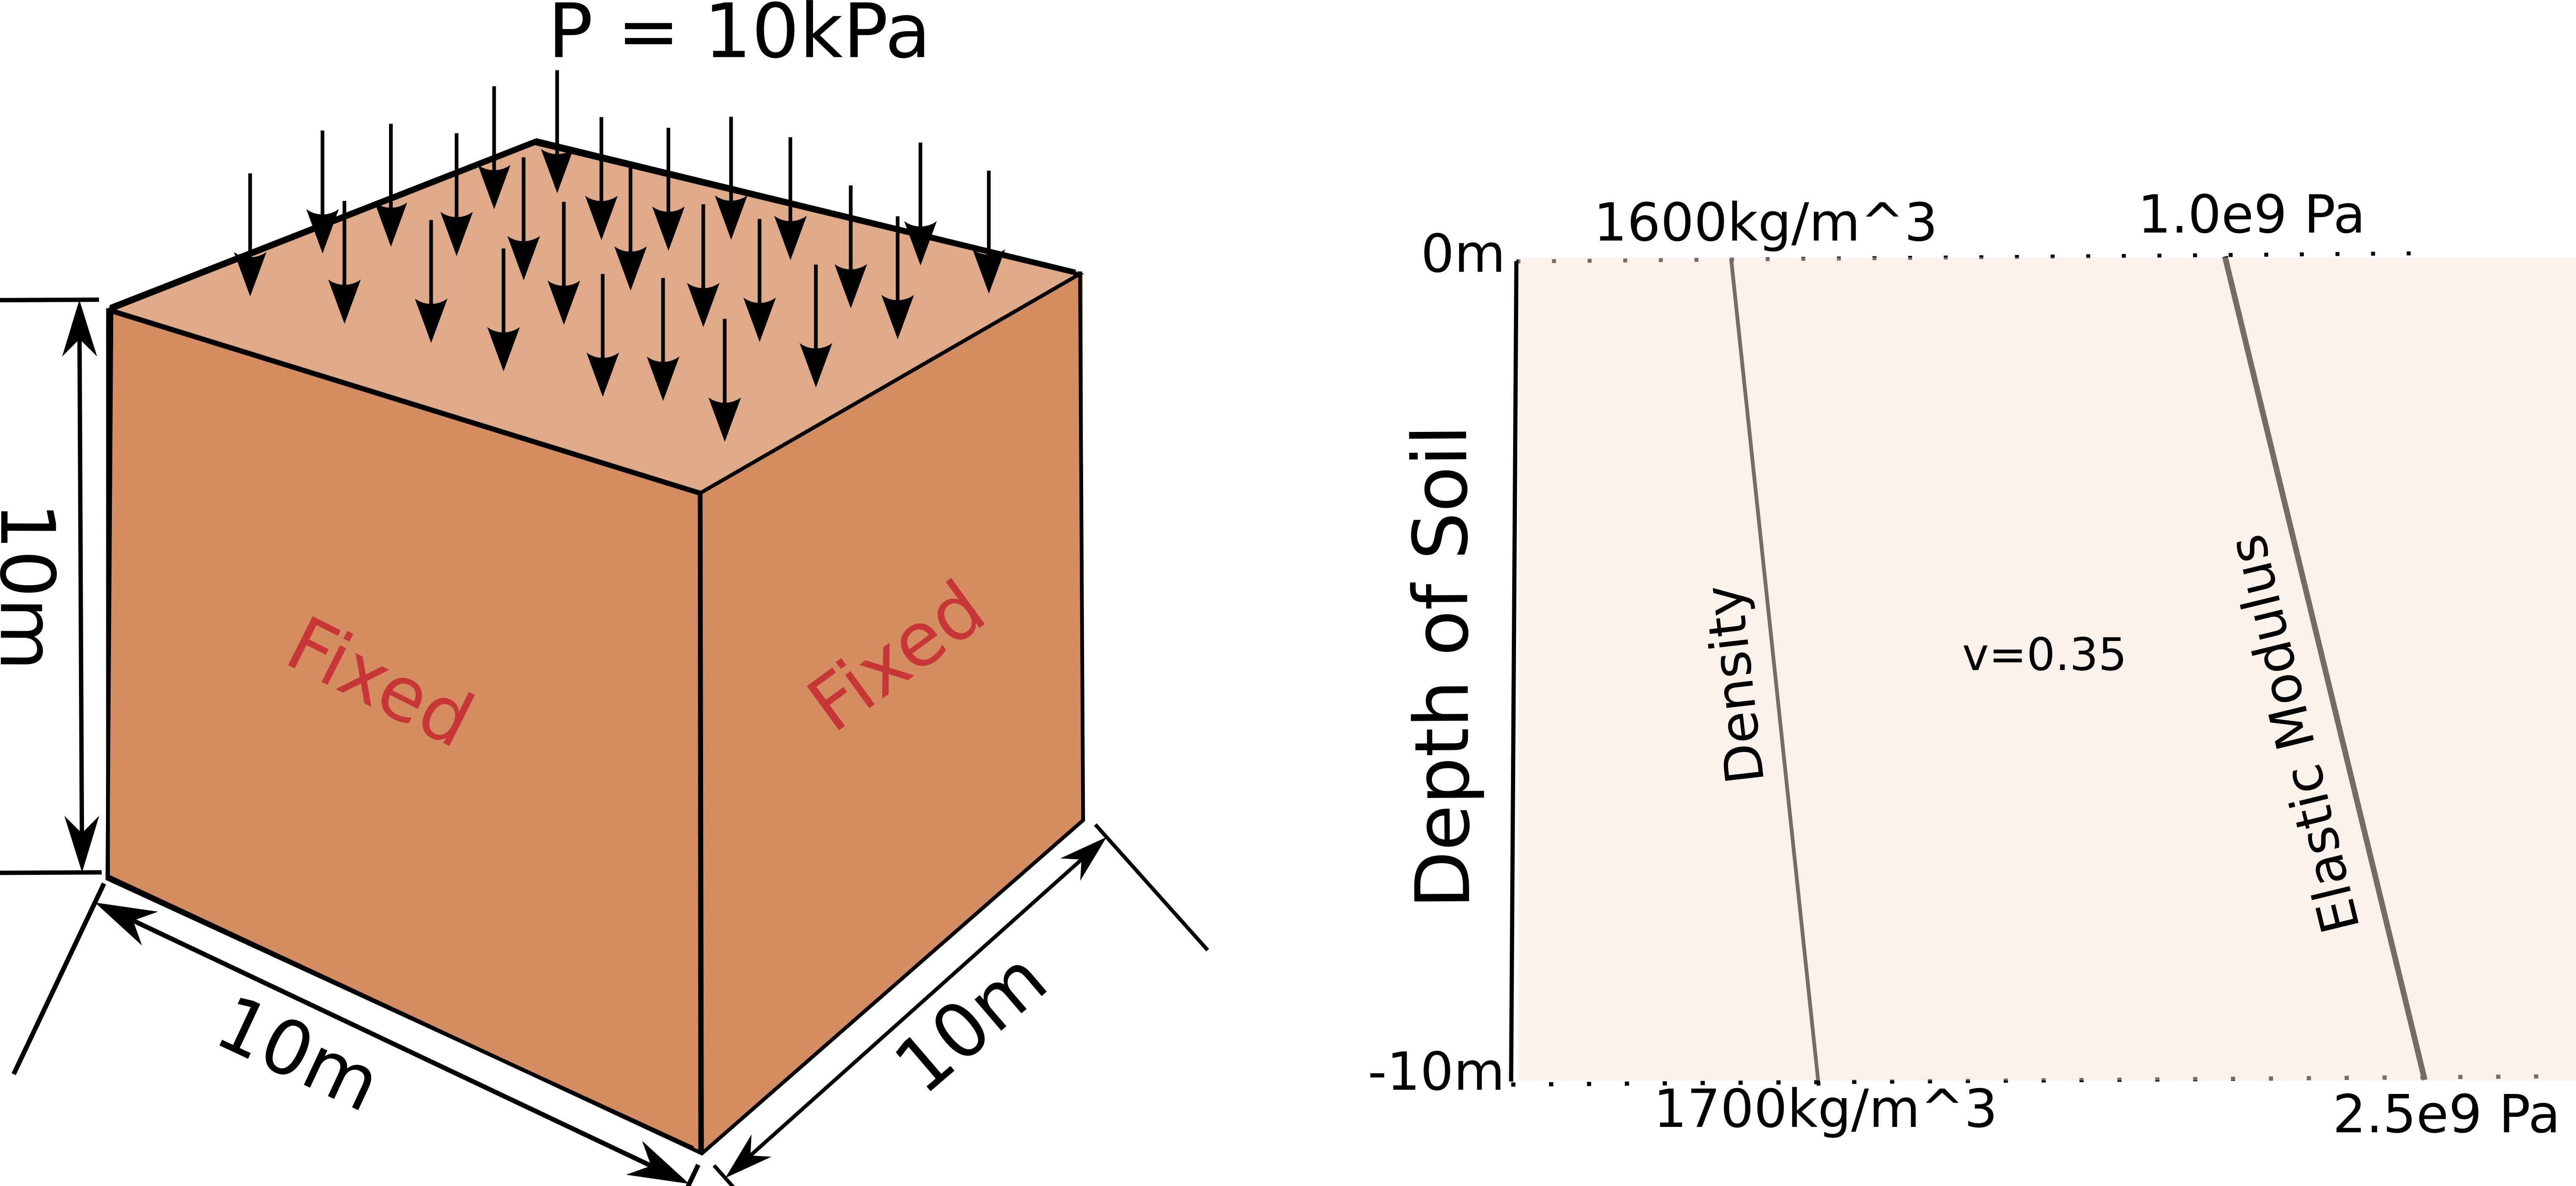
\includegraphics[scale = 0.8]{Images/Example4.png}
\caption{\label{Example4} Description of a Example4}
\end{figure}

It is a block of dimension $10mx10mx10m$ of soil mass whose all 4 lateral faces
and the bottom face are fixed and a surface load of uniform pressure of 10 Pa is
applied. The density and elastic modulus of the soil increases from $1600*kg/m^3$
to $1700*kg/m^3$ and from x to y down the depth as shown in Figure~\ref{Example4}.

%%%%%%%%%%%%%%%%%%%%%%%%%%%%%%%%%%%%%%%%%%%%%%%%%%%%%%%%%%%%%%%%%%%%%%%%%%%%%%%%
\subsection{Making .geo and .msh file in Gmsh}

The first step is to make the geometry file in \textbf{Gmsh}. While creating
the geometry the user should also define all the physical groups on which they
intend to either apply boundary condition, define elements, loads etc. In
Example5, 3 physical groups are needed one for applying surface load, one for
fixities, and one for defining the soil volume and assigning material. The
content of \href
{http://beta.sumeetsinha.in/gmESSI/Examples/Example4/Example4.geo} {
Example4.geo} file is shown below

\begin{lstlisting}[language=C]
$cat Example4.geo 

Point(1) = {0,0,0};

// Extruding and subdividing  each dimension in 10 layers
Extrude{10,0,0}{Point{1}; Layers{10};}
Extrude{0,10,0}{Line{1}; Layers{10};Recombine;}
Extrude{0,0,10}{Surface{5}; Layers{10};Recombine;}

//Creating Physical Groups 
Physical Volume("$SoilVolume$")= {1};
Physical Surface("$Fixities$") = {5,26,18,14,22};
Physical Surface("$SurfaceLoad$") = {27};
\end{lstlisting} 

Once .geo file is ready with all the physical groups, next step is to mesh the
model. The model can be messed from the terminal directly by running gmsh
Example4.geo -3. A quick look at the \href
{http://beta.sumeetsinha.in/gmESSI/Examples/Example4/Example4.msh} {
Example4.msh} file conatining physical groups is shown below.

\begin{lstlisting}[language=C]
$cat Example4.geo 
..............
$PhysicalNames
3
2 2 "$Fixities$"
2 3 "$SurfaceLoad$"
3 1 "$SoilVolume$"
$EndPhysicalNames
................
\end{lstlisting} 


\begin{figure}[h]

  \centering

  \begin{subfigure}[b]{0.3\textwidth}
    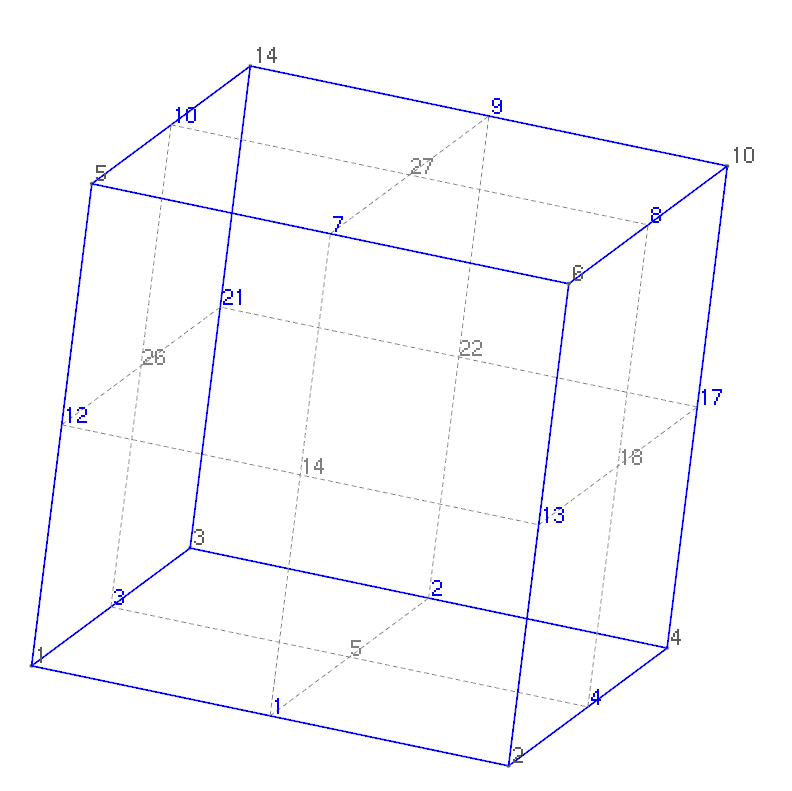
\includegraphics[width=\textwidth]
    {Images/Example4-GeoFile.png}
    \caption{Geometry File}
  \end{subfigure}

  \begin{subfigure}[b]{0.3\textwidth}
    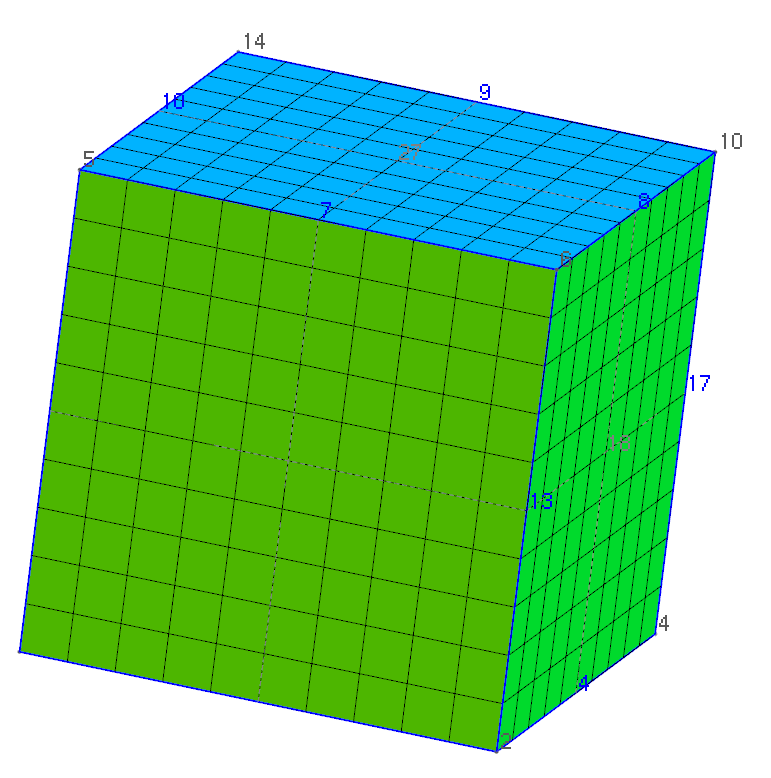
\includegraphics[width=\textwidth]
    {Images/Example4-MeshFile.png}
    \caption{Mesh File}
  \end{subfigure}

\caption{\label{Example4Mesh} Description of a Example4}
\end{figure}

Figure~\ref{Example4Mesh} shows the geometry and mesh visualization in
gmsh.

%%%%%%%%%%%%%%%%%%%%%%%%%%%%%%%%%%%%%%%%%%%%%%%%%%%%%%%%%%%%%%%%%%%%%%%%%%%%%%%%
\subsection{Translataing .msh file using gmESSI to ESSI files}

Using gmESSI for mesh conversion is very easy. To achieve this, the step is
further subdivided into two simpler substeps i.e. creating a
\href{http://beta.sumeetsinha.in/gmESSI/Examples/Example4/Example4.gmessi} {
Example4.gmessi} file containing all the required gmESSI commands to be executed
sequentially and
\href{http://beta.sumeetsinha.in/gmESSI/Examples/Example4/Example4.py} {
Example4.py} file for importing gmESSI python module and executing each gmESSI
command sequentially from file Exampl4.gmessi. Let us look at each of them one
by one.

%%%%%%%%%%%%%%%%%%%%%%%%%%%%%%%%%%%%%%%%%%%%%%%%%%%%%%%%%%%%%%%%%%%%%%%%%%%%%%%%
\subsubsection{Writting all gmESSI Commands for the model}

gmESSI commands for this particular problem is written in   \href
{http://beta.sumeetsinha.in/gmESSI/Examples/Example4/Example4.gmessi} {
Example4.gmessi} file. Since physical group names and ids are required for
referring the gmESSI commands, its always best to copy all the physical group
data from the .msh file (in this case \href
{http://beta.sumeetsinha.in/gmESSI/Examples/Example4/Example4.msh} {
Example4.msh} file) in the header of .gmessi file, so that its easier for the
user to refer to the physical groups while writing commands in .gmessi file. The
contents of the \href
{http://beta.sumeetsinha.in/gmESSI/Examples/Example4/Example4.gmessi} {
Example4.gmessi} are shown below.

\begin{lstlisting}[language=C]
$cat Example4.gmessi 
/////////////////////////////////////////////////////////
//2 2 "$Fixities$"
//2 3 "$SurfaceLoad$"
//3 1 "$SoilVolume$"
/////////////////////////////////////////////////////////

//Adding Model Name
[Model_Name{"Example4"}]
[New_Line{}] 

//Adding all nodes of the model
[Add_All_Node{m,3}]

//Defining and creating 8-noded brick elements with different material properties
[Vary_Linear_elastic_isotropic_3d_LT{ Physical_Group#1, Add_8NodeBrickLT{},
  1600+10*(10-z)\0\kg/m^3, 1.0e9+1.5e8*(10-z)\-8\Pa, 0.35}]
[New_Line{}] 

//Applying Fixities to the model
[Fix{Physical_Group#2,all}]

//Including the geometry file generated
[Include{"Example4_geometry.fei"}]

[New_Line{}] 
[New_Line{}] 

//Adding new loading stage
[Add_New_Loading_Stage{"Stage1_Surface_Loading"}]
[New_Line{}] 

// Adding surface load on the soil mass
[Add_8NodeBrick_SurfaceLoad{Physical_Group#1,Physical_Group#3,10*Pa]

//Including the load file generated
[Include{"Example4_load.fei"}]
[New_Line{}] 
[New_Line{}] 

// Just a comment inside the _analysis file.
[Comment{Starting the simulation}] 
[New_Line{}] 

// Defining algorithms for the model
[Define_Algorithm{With_no_convergence_check}]
[Define_Solver_UMFPack{}]
[New_Line{}] 
[Define_Load_Factor_increament{1}]
[Simulate_Steps_Using_Static_Algorithm{10}]

// A nice good bye
[Bye{}] 
\end{lstlisting} 

\paragraph{Please Note - } The gmESSI commands are executed and
written to the file sequentially, so the user should be carefull with the order
of translation.
%%%%%%%%%%%%%%%%%%%%%%%%%%%%%%%%%%%%%%%%%%%%%%%%%%%%%%%%%%%%%%%%%%%%%%%%%%%%%%%%
\subsubsection{Import gmESSI in python and carrying out Translation}

Once .gmessi is ready, the next task is to make a small python script to import
gmeSSI module and read the commands from .gmessi file and carry out the
convesion. The python script for this problem is written to file \href
{http://beta.sumeetsinha.in/gmESSI/Examples/Example4/Example4.py} {
Example4.py}

\begin{lstlisting}[language=python]
$cat Example4.py
import gmessi

Example4 = gmessi.gmESSIPython()

Example4.loadMshFile("Example4.msh")

Inputfile = open('Example4.gmessi', 'r')

# Skipping the blank line and line with comments (//)
for line in Inputfile:
	line = line.partition('//')[0]
	line = line.rstrip()
	if (line):
		Example4.Convert(line)
\end{lstlisting} 

The next step is to run the python script. Running the python script would
carryout the translation to all gmESSI commands in .gmessi file. The log of
translation gets displayed on the terminal

\begin{lstlisting}[language=bash]
$python Example4.py
Message::Files converted to  
/home/sumeet/sumeet.kumar507@gmail.com/git/gmESSI/Example4_ESSI_Simulation  

Model_Name{"Example4"} Found!!    Sucessfully Converted
New_Line{}                        Found!!    Sucessfully Converted
Add_All_Node{m,3}                 Found!!    Sucessfully Converted
Vary_Linear_elastic_isotropic_3d_LT{ Physical_Group#1, Add_8NodeBrickLT{},
  1600+10*(10-z)\0\kg/m^3, 1.0e9+1.5e8*(10-z)\-8\Pa, 0.35} Found!!  Sucessfully
	Converted
New_Line{}                        Found!!    Sucessfully Converted
Fix{Physical_Group#2,all}         Found!!    Sucessfully Converted
Include{"Example4_geometry.fei"}	 Found!!    Sucessfully Converted
New_Line{}  Found!!    Sucessfully Converted
New_Line{}  Found!!    Sucessfully Converted
Add_New_Loading_Stage{"Stage1_Surface_Loading"}	 Found!!    Sucessfully
Converted
New_Line{}  Found!!    Sucessfully Converted
Add_8NodeBrick_SurfaceLoad{Physical_Group#1,Physical_Group#3,10*Pa Found!!   
	Sucessfully Converted
Include{"Example4_load.fei"}  Found!!    Sucessfully Converted
New_Line{}  Found!!    Sucessfully Converted
New_Line{}  Found!!    Sucessfully Converted
Comment{Starting the simulation}   Found!!    Sucessfully Converted
New_Line{}  Found!!    Sucessfully Converted
Define_Algorithm{With_no_convergence_check}	 Found!!    Sucessfully Converted
Define_SolveFound!!    Sucessfully Converted
New_Line{}  Found!!    Sucessfully Converted
Define_Load_Factor_increament{1}  Found!!    Sucessfully Converted
Simulate_Steps_Using_Static_Algorithm{10}Found!!    Sucessfully Converted
Bye{}       Found!!    Sucessfully Converted


************************ Updated New Tag Numberring *********************
damping         = 1
displacement    = 1
element         = 701
field           = 1
load            = 101
material        = 11
motion          = 1
node            = 1332
nodes           = 1332

\end{lstlisting} 

Running gmESSI creates a folder \href
{http://beta.sumeetsinha.in/gmESSI/Examples/Example4/Example4_ESSI_Simulation} {
Example4_ESSI_Simulation} and places \href
{http://beta.sumeetsinha.in/gmESSI/Examples/Example4/Example4_ESSI_Simulation/Example4_load.fei} {
Example4_load.fei} file, \href
{http://beta.sumeetsinha.in/gmESSI/Examples/Example4/Example4_ESSI_Simulation/Example4_geometry.fei} {
Example4_geometry.fei} file and \href
{http://beta.sumeetsinha.in/gmESSI/Examples/Example4/Example4_ESSI_Simulation/Example4_analysis.fei} {
Example4_analysis.fei} i.e. ESSI main file. The user at this point do not need
to write anything in the Example4_analysis.fei file as every command was
sequentially written down in .gmessi file and is converted. 


Please note that
material variational commands has created exactly 10 different material
layer-wise with increasing densitty and elastic modulus. The content of the
main analysis.fei file is shown below

\begin{lstlisting}[language=C]
$cat Example4_analysis.fei
model name "Example4";
; 
add material #1 type linear_elastic_isotropic_3d_LT mass_density=1695.000000*kg/m^3 elastic_modulus=2420000000.000000*Pa poisson_ratio=0.35;  
add material #2 type linear_elastic_isotropic_3d_LT mass_density=1685.000000*kg/m^3 elastic_modulus=2280000000.000000*Pa poisson_ratio=0.35;  
add material #3 type linear_elastic_isotropic_3d_LT mass_density=1675.000000*kg/m^3 elastic_modulus=2120000000.000000*Pa poisson_ratio=0.35;  
add material #4 type linear_elastic_isotropic_3d_LT mass_density=1665.000000*kg/m^3 elastic_modulus=1980000000.000000*Pa poisson_ratio=0.35;  
add material #5 type linear_elastic_isotropic_3d_LT mass_density=1655.000000*kg/m^3 elastic_modulus=1820000000.000000*Pa poisson_ratio=0.35;  
add material #6 type linear_elastic_isotropic_3d_LT mass_density=1645.000000*kg/m^3 elastic_modulus=1680000000.000000*Pa poisson_ratio=0.35;  
add material #7 type linear_elastic_isotropic_3d_LT mass_density=1635.000000*kg/m^3 elastic_modulus=1520000000.000000*Pa poisson_ratio=0.35;  
add material #8 type linear_elastic_isotropic_3d_LT mass_density=1625.000000*kg/m^3 elastic_modulus=1380000000.000000*Pa poisson_ratio=0.35;  
add material #9 type linear_elastic_isotropic_3d_LT mass_density=1615.000000*kg/m^3 elastic_modulus=1220000000.000000*Pa poisson_ratio=0.35;  
add material #10 type linear_elastic_isotropic_3d_LT mass_density=1605.000000*kg/m^3 elastic_modulus=1080000000.000000*Pa poisson_ratio=0.35; 
; 
include "Example4_geometry.fei";
; 
; 
new loading stage "Stage1_Surface_Loading";
; 
include "Example4_load.fei";
; 
; 
 //Starting the simulation;
; 
define algorithm With_no_convergence_check;
define solver UMFPack;
; 
define load factor increment 1;
simulate 10 steps using static algorithm;
bye; 	
\end{lstlisting}

%%%%%%%%%%%%%%%%%%%%%%%%%%%%%%%%%%%%%%%%%%%%%%%%%%%%%%%%%%%%%%%%%%%%%%%%%%%%%%%%
\subsection{Running ESSI and visualization in visit}

With all files ready in their place, the next step is to run the
Example4_analysis.fei file directly in ESSI. 

\begin{lstlisting}[language=bash]
$essi -f Example4_analysis.fei
                                                              
                                                               
  The Finite Element Interpreter                               
                                                               
  Real ESSI                                                  
  Earthquake Soil Structure Interaction Simulator            
                                                             
  Sequential processing mode.                                
                                                             
Compiled: Jun 15 2015 at 15:28:24
Time Now: Aug 28 2015 at 19:09:57
                                                               
Static startup tips:                                           
 * Remember: Every command ends with a semicolon ';'.          
 * Type 'quit;' or 'exit;' to finish.                          
 * Run 'essi -h to see available command line options.        
                                                               
Input: STDIN

Including: "Example4_analysis.fei"


Model name is being set to "Example4"

Including: "Example4_geometry.fei"

Done including: "Example4_geometry.fei" (2352 lines included).
Continuing with "Example4_analysis.fei" at line 16.



Starting new stage: Stage1_Surface_Loading

Including: "Example4_load.fei"

Done including: "Example4_load.fei" (642 lines included).
Continuing with "Example4_analysis.fei" at line 22.


Starting sequential static multistep analysis
====================================================================
Creating analysis model...................................................Pass!
Checking constraint handler...............................................Pass!
Checking numberer.........................................................Pass!
Checking analysis algorithm...............................................Pass!
Checking system of equation handler.......................................Pass!
Checking transient integration handler....................................Pass!
setNumberOfOutputSteps ->  nsteps / output_every_nsteps = 10
Static Analysis: Step Number is : 1 out of 10Domain::update( void ) -- Constitutive integration happening!
Static Analysis: Step Number is : 2 out of 10Domain::update( void ) -- Constitutive integration happening!
Static Analysis: Step Number is : 3 out of 10Domain::update( void ) -- Constitutive integration happening!

\end{lstlisting}

Running ESSI creates .feioutput file which can be visualized in visit software.
Figure~\ref{Example4Visit} shows the visualization of \href
{http://beta.sumeetsinha.in/gmESSI/Examples/Example4/Example4_ESSI_Simulation/Example4_Stage1_Surface_Loading.h5.feioutput} {
Example4_Stage1_Surface_Loading.h5.feioutput} produced in visit.

\begin{figure}[h]
  
  \centering
  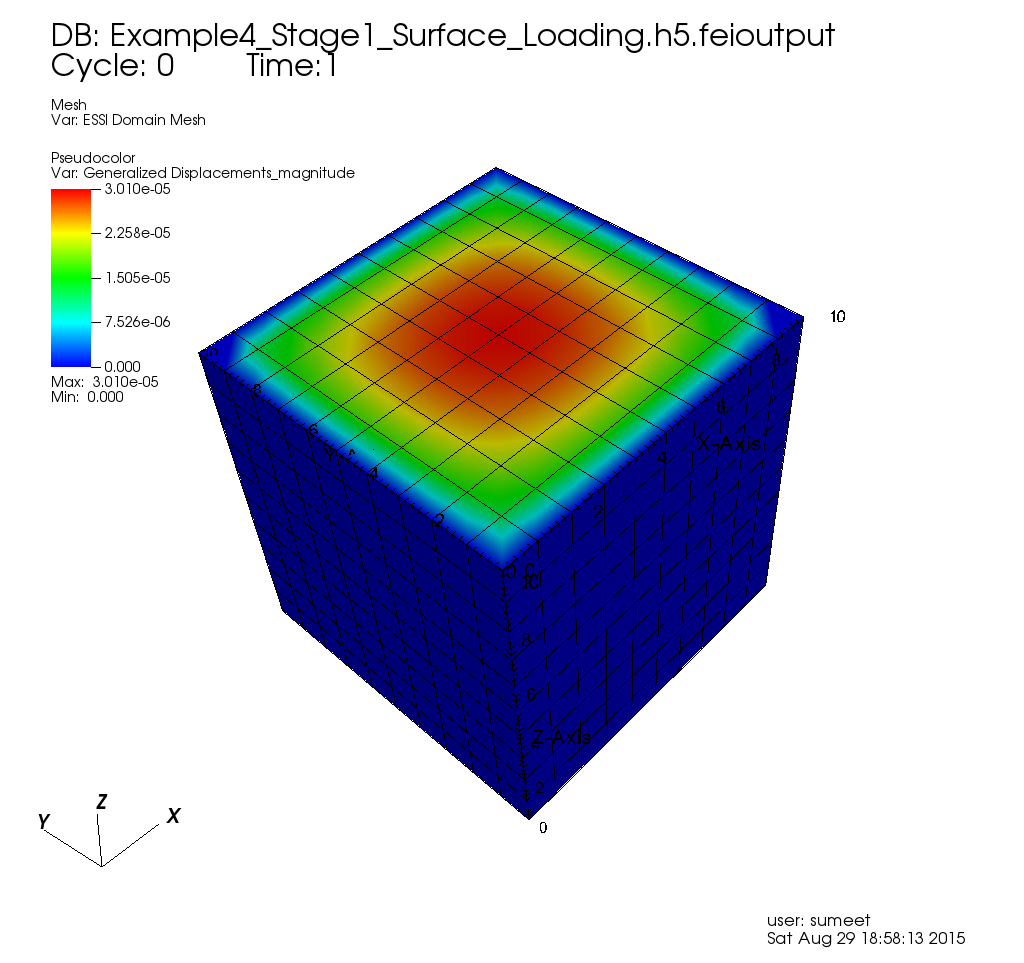
\includegraphics[scale=0.4]{Images/Example4-visit.png}
  \caption{\label{Example4Visit} Visualizing output in visit}

\end{figure}

\end{document}
